\documentclass[twoside]{book}

% Packages required by doxygen
\usepackage{fixltx2e}
\usepackage{calc}
\usepackage{doxygen}
\usepackage[export]{adjustbox} % also loads graphicx
\usepackage{graphicx}
\usepackage[utf8]{inputenc}
\usepackage{makeidx}
\usepackage{multicol}
\usepackage{multirow}
\PassOptionsToPackage{warn}{textcomp}
\usepackage{textcomp}
\usepackage[nointegrals]{wasysym}
\usepackage[table]{xcolor}

% NLS support packages
\usepackage[ngerman]{babel}

% Font selection
\usepackage[T1]{fontenc}
\usepackage[scaled=.90]{helvet}
\usepackage{courier}
\usepackage{amssymb}
\usepackage{sectsty}
\renewcommand{\familydefault}{\sfdefault}
\allsectionsfont{%
  \fontseries{bc}\selectfont%
  \color{darkgray}%
}
\renewcommand{\DoxyLabelFont}{%
  \fontseries{bc}\selectfont%
  \color{darkgray}%
}
\newcommand{\+}{\discretionary{\mbox{\scriptsize$\hookleftarrow$}}{}{}}

% Page & text layout
\usepackage{geometry}
\geometry{%
  a4paper,%
  top=2.5cm,%
  bottom=2.5cm,%
  left=2.5cm,%
  right=2.5cm%
}
\tolerance=750
\hfuzz=15pt
\hbadness=750
\setlength{\emergencystretch}{15pt}
\setlength{\parindent}{0cm}
\setlength{\parskip}{3ex plus 2ex minus 2ex}
\makeatletter
\renewcommand{\paragraph}{%
  \@startsection{paragraph}{4}{0ex}{-1.0ex}{1.0ex}{%
    \normalfont\normalsize\bfseries\SS@parafont%
  }%
}
\renewcommand{\subparagraph}{%
  \@startsection{subparagraph}{5}{0ex}{-1.0ex}{1.0ex}{%
    \normalfont\normalsize\bfseries\SS@subparafont%
  }%
}
\makeatother

% Headers & footers
\usepackage{fancyhdr}
\pagestyle{fancyplain}
\fancyhead[LE]{\fancyplain{}{\bfseries\thepage}}
\fancyhead[CE]{\fancyplain{}{}}
\fancyhead[RE]{\fancyplain{}{\bfseries\leftmark}}
\fancyhead[LO]{\fancyplain{}{\bfseries\rightmark}}
\fancyhead[CO]{\fancyplain{}{}}
\fancyhead[RO]{\fancyplain{}{\bfseries\thepage}}
\fancyfoot[LE]{\fancyplain{}{}}
\fancyfoot[CE]{\fancyplain{}{}}
\fancyfoot[RE]{\fancyplain{}{\bfseries\scriptsize Erzeugt von Doxygen }}
\fancyfoot[LO]{\fancyplain{}{\bfseries\scriptsize Erzeugt von Doxygen }}
\fancyfoot[CO]{\fancyplain{}{}}
\fancyfoot[RO]{\fancyplain{}{}}
\renewcommand{\footrulewidth}{0.4pt}
\renewcommand{\chaptermark}[1]{%
  \markboth{#1}{}%
}
\renewcommand{\sectionmark}[1]{%
  \markright{\thesection\ #1}%
}

% Indices & bibliography
\usepackage{natbib}
\usepackage[titles]{tocloft}
\setcounter{tocdepth}{3}
\setcounter{secnumdepth}{5}
\makeindex

% Custom commands
\newcommand{\clearemptydoublepage}{%
  \newpage{\pagestyle{empty}\cleardoublepage}%
}

\usepackage{caption}
\captionsetup{labelsep=space,justification=centering,font={bf},singlelinecheck=off,skip=4pt,position=top}

%===== C O N T E N T S =====

\begin{document}

% Titlepage & ToC
\pagenumbering{alph}
\begin{titlepage}
\vspace*{7cm}
\begin{center}%
{\Large S\+Q\+L-\/\+Library }\\
\vspace*{1cm}
{\large Erzeugt von Doxygen 1.8.14}\\
\end{center}
\end{titlepage}
\clearemptydoublepage
\pagenumbering{roman}
\tableofcontents
\clearemptydoublepage
\pagenumbering{arabic}

%--- Begin generated contents ---
\chapter{Hauptseite}
\label{index}~\newline
 {\bfseries  ---Vorwort--- }

Selektierung von C++ und der Standard-\/\+Bibliothek von My\+S\+QL.~\newline
 S\+Q\+L-\/\+Statements können über Methoden und Parameter abgearbeitet werden.~\newline
 Bedienbar entweder über die Konsole und den einfachen Methoden-\/\+Aufruf oder über das Interface.~\newline


~\newline


{\bfseries  ---Einrichtung--- }

Der Socket für X\+A\+M\+PP auf Linux sowie M\+A\+MP auf Mac\+OS wurden bereits implementiert falls diese Bibliothek local genutzt werden soll.~\newline


Sollte die Anwendung nicht Lokal genutzt werden, muss der Ort an dem der spezifische S\+Q\+L-\/\+Socket ~\newline
 clientseitig liegt identifiziert werden um mit dem S\+Q\+L-\/\+Server zu kommunizieren.~\newline
 Für den Verbindungsaufbau wird die connectionless-\/\+Methode \doxyref{connectionless()}{S.}{connection_8cpp_a4ec2c49f65ab04fdddbdb7e81e6aab18} (siehe Übergabe-\/\+Parameter) der connection-\/\+Klasse ~\newline
 benutzt, diese baut nach der Build-\/\+Routine bei der Ausführung des Programm\textquotesingle{}s eine Verbindung auf.~\newline


Durch vorgefertigte Präprozessor-\/\+Direktiven wird für Mac\+O\+S-\// sowie Linuxbetriebssysteme der zu benötigende My\+S\+Q\+L-\/\+Header beim kompilieren direkt rausgesucht. ~\newline
 ~\newline
 In der Regel sollte der My\+S\+Q\+L-\/\+Header im Standardpfad des dementsprechenden Betriebssystems liegen. ~\newline
 Sollte dies nicht der Fall sein, muss die Variable in der \doxyref{connectionless()}{S.}{connection_8cpp_a4ec2c49f65ab04fdddbdb7e81e6aab18} Methode gelöscht und durch eine eigene Variable (String des Pfads + mysql.\+h) ersetzt werden.~\newline


Für das Ausführen des Programms ohne Benutzeroberfläche wird das erstellte Shellscript mit den dementsprechenden Umgebungsvariablen benutzt.~\newline
 Sollte, wie vorher beschrieben der Pfad für den My\+S\+Q\+L-\/\+Header nicht im Standardpfad liegen, muss ebenfalls das Shellscript angepasst werden. ~\newline
 Die Bedingung im Shellscript sieht vor, dass je nach Pfad für die mysql.\+h andere Compiler-\/\+Optionen vorgenommen werden. ~\newline
 Hier muss lediglich der Pfad mit inbegriffender Header-\/\+Datei eingebunden werden um das Shellscript lauffähig zu bekommen. ~\newline
 Für die Ausführung des User-\/\+Interfaces steht ein eigens entwickeltes Shellscript zur verfügung. ~\newline


!\+Kein Support für Microsoft-\/\+Betriebssysteme!

~\newline


{\bfseries  ---Nice to know--- }

Da in diesem Projekt ausschließlich mit der My\+S\+Q\+L-\/\+Standardbibliothek gearbeitet wurde, passiert die Fehlerausgabe über die \doxyref{check\+\_\+error()}{S.}{connection_8cpp_a88c581f1a3f4e5319ab41c2cc8ef67af} Methode.~\newline
 Diese fängt jegliche Fehlerausgaben des My\+S\+Q\+L-\/\+Servers ab und printed diese aus. ~\newline
 ~\newline
 Sollte dieses Programm über die Konsole genutzt werden, müssen jegliche Übergabeparameter (ausgeschlossen Integer) in einen String gepackt werden. (\char`\"{} \char`\"{})~\newline
 Durch die Benutzung des Interfaces kann diese Anweisung jedoch ignoriert werden. ~\newline
 ~\newline


\begin{DoxyAuthor}{Autor}
Steffen Extra 

Martin Meyer 
\end{DoxyAuthor}

\chapter{Datei-\/\+Verzeichnis}
\section{Auflistung der Dateien}
Hier folgt die Aufzählung aller Dateien mit einer Kurzbeschreibung\+:\begin{DoxyCompactList}
\item\contentsline{section}{\textbf{ connection.\+cpp} }{\pageref{connection_8cpp}}{}
\item\contentsline{section}{\textbf{ database.\+cpp} }{\pageref{database_8cpp}}{}
\item\contentsline{section}{\textbf{ entry.\+cpp} }{\pageref{entry_8cpp}}{}
\item\contentsline{section}{\textbf{ main.\+cpp} }{\pageref{main_8cpp}}{}
\item\contentsline{section}{\textbf{ selection\+Request.\+cpp} }{\pageref{selection_request_8cpp}}{}
\item\contentsline{section}{\textbf{ sqllib.\+hpp} }{\pageref{sqllib_8hpp}}{}
\item\contentsline{section}{\textbf{ tables.\+cpp} }{\pageref{tables_8cpp}}{}
\end{DoxyCompactList}

\chapter{Datei-\/\+Dokumentation}
\section{connection.\+cpp-\/\+Dateireferenz}
\label{connection_8cpp}\index{connection.\+cpp@{connection.\+cpp}}
{\ttfamily \#include \char`\"{}sqllib.\+hpp\char`\"{}}\newline
Include-\/\+Abhängigkeitsdiagramm für connection.\+cpp\+:\nopagebreak
\begin{figure}[H]
\begin{center}
\leavevmode
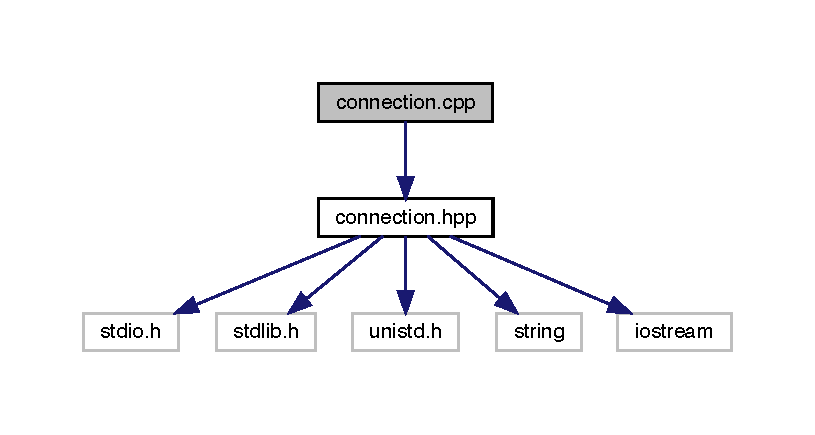
\includegraphics[width=350pt]{connection_8cpp__incl}
\end{center}
\end{figure}
\subsection*{Funktionen}
\begin{DoxyCompactItemize}
\item 
std\+::string \textbf{ check\+\_\+error} (void)
\begin{DoxyCompactList}\small\item\em Fehlermethode. \end{DoxyCompactList}\item 
std\+::string \textbf{ connection\+\_\+feedback} (std\+::string sql\+Command)
\begin{DoxyCompactList}\small\item\em Rückgabe einzelner Ergebnisse. \end{DoxyCompactList}\item 
std\+::string \textbf{ connection\+\_\+feedback\+All} (std\+::string sql\+Command)
\begin{DoxyCompactList}\small\item\em Rückgabe aller Datensätze. \end{DoxyCompactList}\item 
std\+::string \textbf{ connection\+\_\+query} (std\+::string sql\+Command)
\begin{DoxyCompactList}\small\item\em Sendet eine Abfrage zum S\+Q\+L-\/\+Server. \end{DoxyCompactList}\item 
bool \textbf{ connectionless} (const char host [$\,$], const char user [$\,$], const char passwort [$\,$], const char db [$\,$], unsigned int port, const char $\ast$mac\+O\+S\+\_\+socket, unsigned int client\+\_\+flag)
\begin{DoxyCompactList}\small\item\em Verbindung zur Datenbank auf einem Server. \end{DoxyCompactList}\item 
void \textbf{ disconnect} ()
\begin{DoxyCompactList}\small\item\em Verbindung schließen. \end{DoxyCompactList}\end{DoxyCompactItemize}
\subsection*{Variablen}
\begin{DoxyCompactItemize}
\item 
M\+Y\+S\+QL $\ast$ \textbf{ mysql}
\begin{DoxyCompactList}\small\item\em Variable für die Schnittstelle zum S\+Q\+L-\/\+Server. \end{DoxyCompactList}\item 
M\+Y\+S\+Q\+L\+\_\+\+R\+OW \textbf{ row}
\begin{DoxyCompactList}\small\item\em Erhält als Ergebnis einer Reihe von einem Result-\/\+Set. \end{DoxyCompactList}\item 
M\+Y\+S\+Q\+L\+\_\+\+R\+ES $\ast$ \textbf{ result}
\begin{DoxyCompactList}\small\item\em Enthält das Ergebnis einer Abfrage vom S\+Q\+L-\/\+Server. \end{DoxyCompactList}\item 
M\+Y\+S\+Q\+L\+\_\+\+F\+I\+E\+LD $\ast$ \textbf{ field}
\begin{DoxyCompactList}\small\item\em Variable für das Aufrufen der Methode mysql\+\_\+fetch\+\_\+field() um Datenbankinformationen ausgeben zu lassen. \end{DoxyCompactList}\end{DoxyCompactItemize}


\subsection{Dokumentation der Funktionen}
\mbox{\label{connection_8cpp_a88c581f1a3f4e5319ab41c2cc8ef67af}} 
\index{connection.\+cpp@{connection.\+cpp}!check\+\_\+error@{check\+\_\+error}}
\index{check\+\_\+error@{check\+\_\+error}!connection.\+cpp@{connection.\+cpp}}
\subsubsection{check\+\_\+error()}
{\footnotesize\ttfamily std\+::string check\+\_\+error (\begin{DoxyParamCaption}\item[{void}]{ }\end{DoxyParamCaption})}



Fehlermethode. 

Die Methode \char`\"{}check\+\_\+error\char`\"{} ist verantwortlich für die Ausnahme, die ausgelöst wird, wenn My\+S\+QL einen Fehler zurückgibt.~\newline



\begin{DoxyParams}{Parameter}
{\em -\/} & \\
\hline
\end{DoxyParams}
\begin{DoxyReturn}{Rückgabe}
void 
\end{DoxyReturn}
\mbox{\label{connection_8cpp_ad03c38dd32272758034b10850a948786}} 
\index{connection.\+cpp@{connection.\+cpp}!connection\+\_\+feedback@{connection\+\_\+feedback}}
\index{connection\+\_\+feedback@{connection\+\_\+feedback}!connection.\+cpp@{connection.\+cpp}}
\subsubsection{connection\+\_\+feedback()}
{\footnotesize\ttfamily std\+::string connection\+\_\+feedback (\begin{DoxyParamCaption}\item[{std\+::string}]{sql\+Command }\end{DoxyParamCaption})}



Rückgabe einzelner Ergebnisse. 

Die Methode \char`\"{}connection\+\_\+feedback\char`\"{} liefert eine Spalte des aktuellen Datensatzes.~\newline
 Diese wird benutzt um einzelne Ergebnis zurückzugeben. (Bspw. \doxyref{select\+Count()}{S.}{selection_request_8cpp_a00f071477f164f70927ee9923dd77a39} )


\begin{DoxyParams}{Parameter}
{\em sql\+Command} & = enthält den auszuführenden S\+Q\+L-\/\+Befehl\\
\hline
\end{DoxyParams}
\begin{DoxyReturn}{Rückgabe}
void 
\end{DoxyReturn}
Hier ist ein Graph, der zeigt, was diese Funktion aufruft\+:
\nopagebreak
\begin{figure}[H]
\begin{center}
\leavevmode
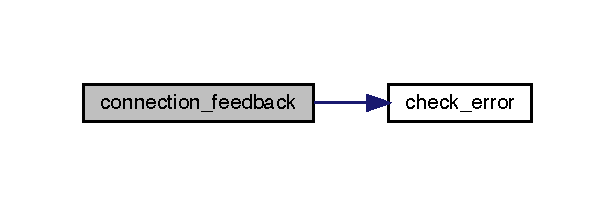
\includegraphics[width=295pt]{connection_8cpp_ad03c38dd32272758034b10850a948786_cgraph}
\end{center}
\end{figure}
Hier ist ein Graph der zeigt, wo diese Funktion aufgerufen wird\+:
\nopagebreak
\begin{figure}[H]
\begin{center}
\leavevmode
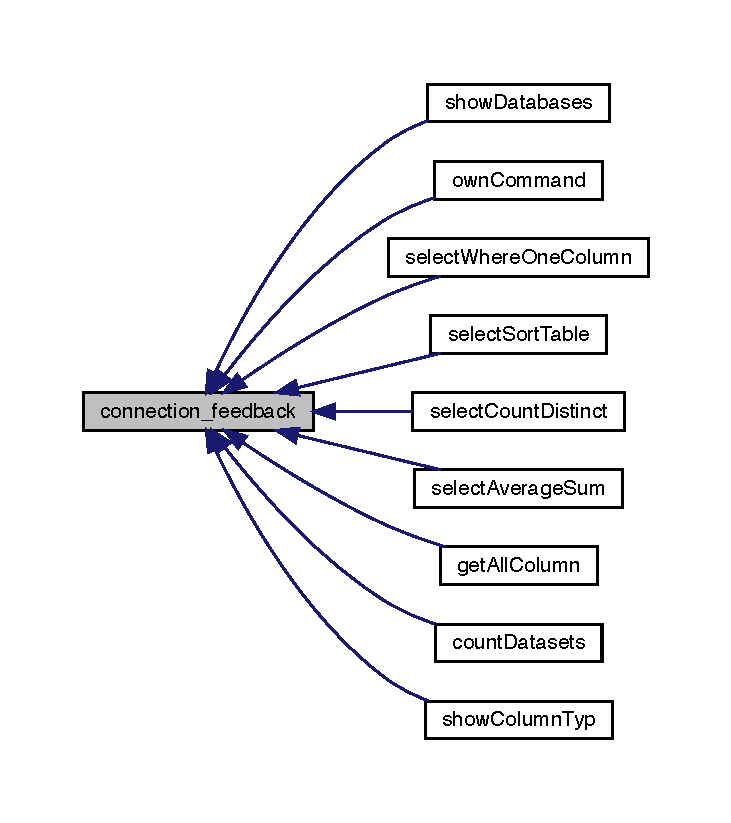
\includegraphics[width=350pt]{connection_8cpp_ad03c38dd32272758034b10850a948786_icgraph}
\end{center}
\end{figure}
\mbox{\label{connection_8cpp_a15d37939fd8d5feac068848fb0e17359}} 
\index{connection.\+cpp@{connection.\+cpp}!connection\+\_\+feedback\+All@{connection\+\_\+feedback\+All}}
\index{connection\+\_\+feedback\+All@{connection\+\_\+feedback\+All}!connection.\+cpp@{connection.\+cpp}}
\subsubsection{connection\+\_\+feedback\+All()}
{\footnotesize\ttfamily std\+::string connection\+\_\+feedback\+All (\begin{DoxyParamCaption}\item[{std\+::string}]{sql\+Command }\end{DoxyParamCaption})}



Rückgabe aller Datensätze. 

Die Methode \char`\"{}connection\+\_\+feedback\+All\char`\"{} liefert den kompletten Datensatz zurück der Abfrage zurück.


\begin{DoxyParams}{Parameter}
{\em sql\+Command} & = enhält den auszuführenden S\+Q\+L-\/\+Befehl\\
\hline
\end{DoxyParams}
\begin{DoxyReturn}{Rückgabe}
void 
\end{DoxyReturn}
Hier ist ein Graph, der zeigt, was diese Funktion aufruft\+:
\nopagebreak
\begin{figure}[H]
\begin{center}
\leavevmode
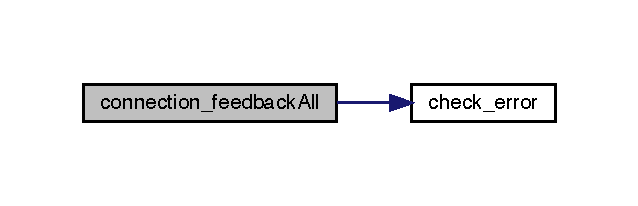
\includegraphics[width=306pt]{connection_8cpp_a15d37939fd8d5feac068848fb0e17359_cgraph}
\end{center}
\end{figure}
Hier ist ein Graph der zeigt, wo diese Funktion aufgerufen wird\+:
\nopagebreak
\begin{figure}[H]
\begin{center}
\leavevmode
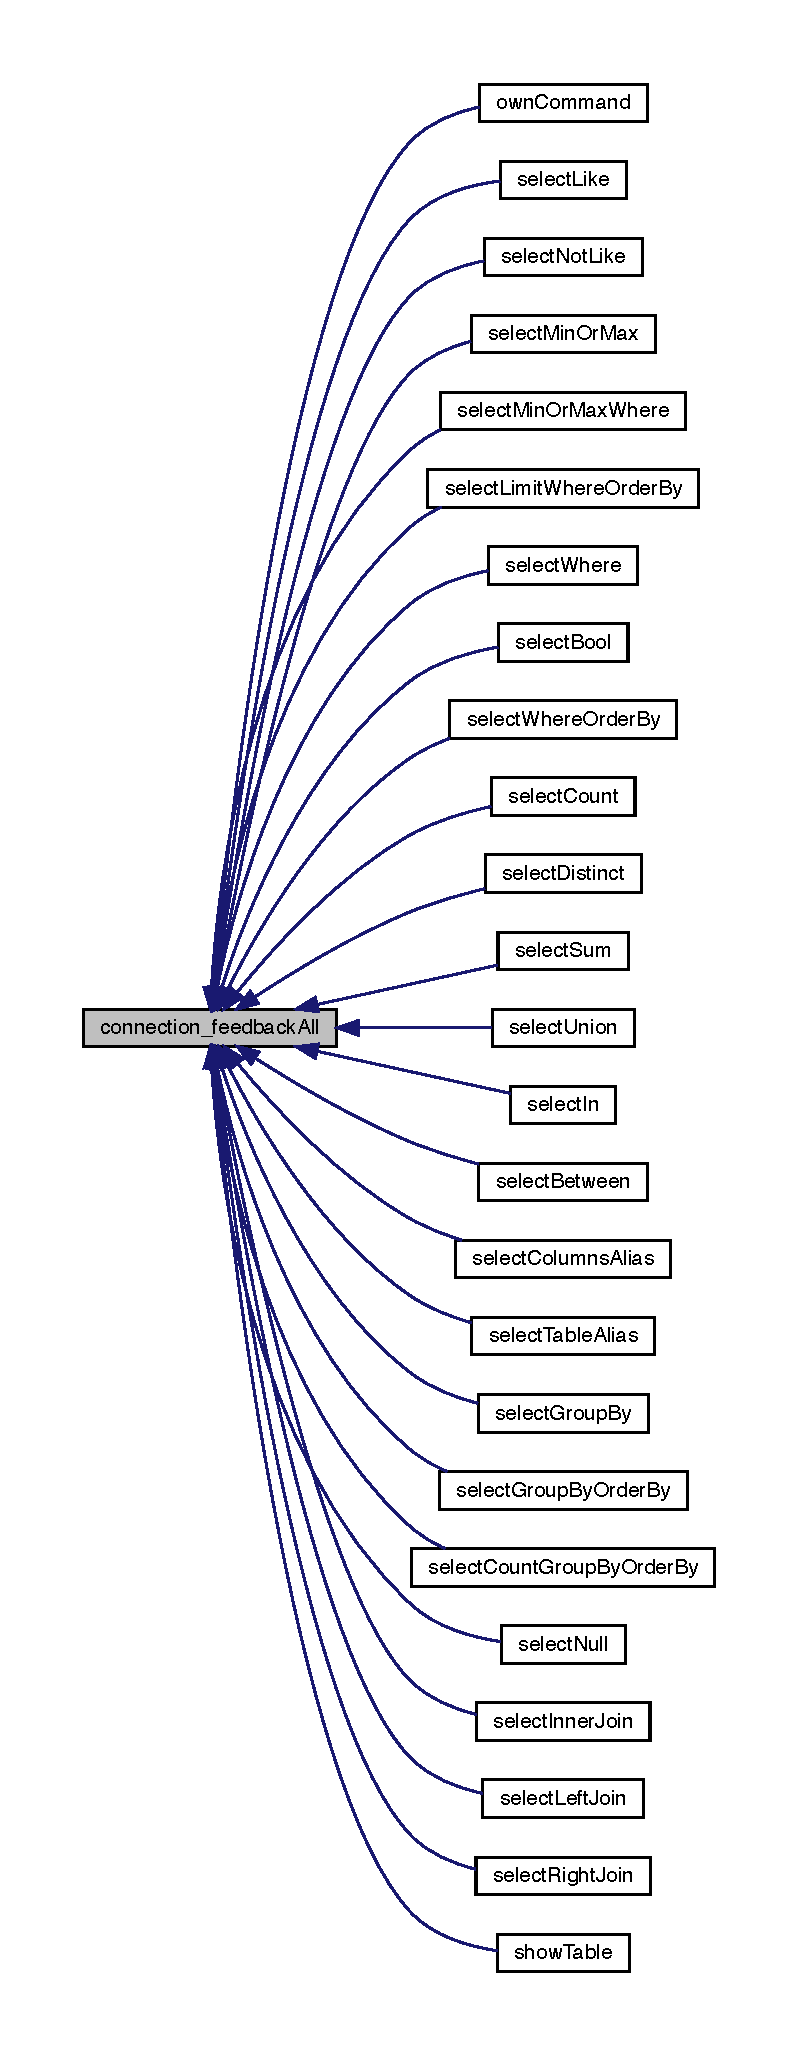
\includegraphics[height=550pt]{connection_8cpp_a15d37939fd8d5feac068848fb0e17359_icgraph}
\end{center}
\end{figure}
\mbox{\label{connection_8cpp_a6fbdf23f9e84af310b023db3e03bb749}} 
\index{connection.\+cpp@{connection.\+cpp}!connection\+\_\+query@{connection\+\_\+query}}
\index{connection\+\_\+query@{connection\+\_\+query}!connection.\+cpp@{connection.\+cpp}}
\subsubsection{connection\+\_\+query()}
{\footnotesize\ttfamily std\+::string connection\+\_\+query (\begin{DoxyParamCaption}\item[{std\+::string}]{sql\+Command }\end{DoxyParamCaption})}



Sendet eine Abfrage zum S\+Q\+L-\/\+Server. 

Die Methode \char`\"{}connection\+\_\+query\char`\"{} sendet eine eindeutige Abfrage (mehrere Abfragen werden nicht unterstützt) an die derzeit aktive Datenbank auf dem Server, der dem angegebenen Server zugeordnet ist. ~\newline



\begin{DoxyParams}{Parameter}
{\em sql\+Command} & = enhält den auszuführenden S\+Q\+L-\/\+Befehl\\
\hline
\end{DoxyParams}
\begin{DoxyReturn}{Rückgabe}
void 
\end{DoxyReturn}
Hier ist ein Graph, der zeigt, was diese Funktion aufruft\+:
\nopagebreak
\begin{figure}[H]
\begin{center}
\leavevmode
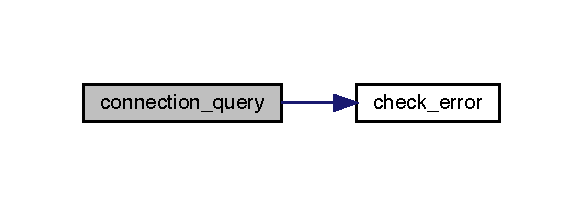
\includegraphics[width=280pt]{connection_8cpp_a6fbdf23f9e84af310b023db3e03bb749_cgraph}
\end{center}
\end{figure}
Hier ist ein Graph der zeigt, wo diese Funktion aufgerufen wird\+:
\nopagebreak
\begin{figure}[H]
\begin{center}
\leavevmode
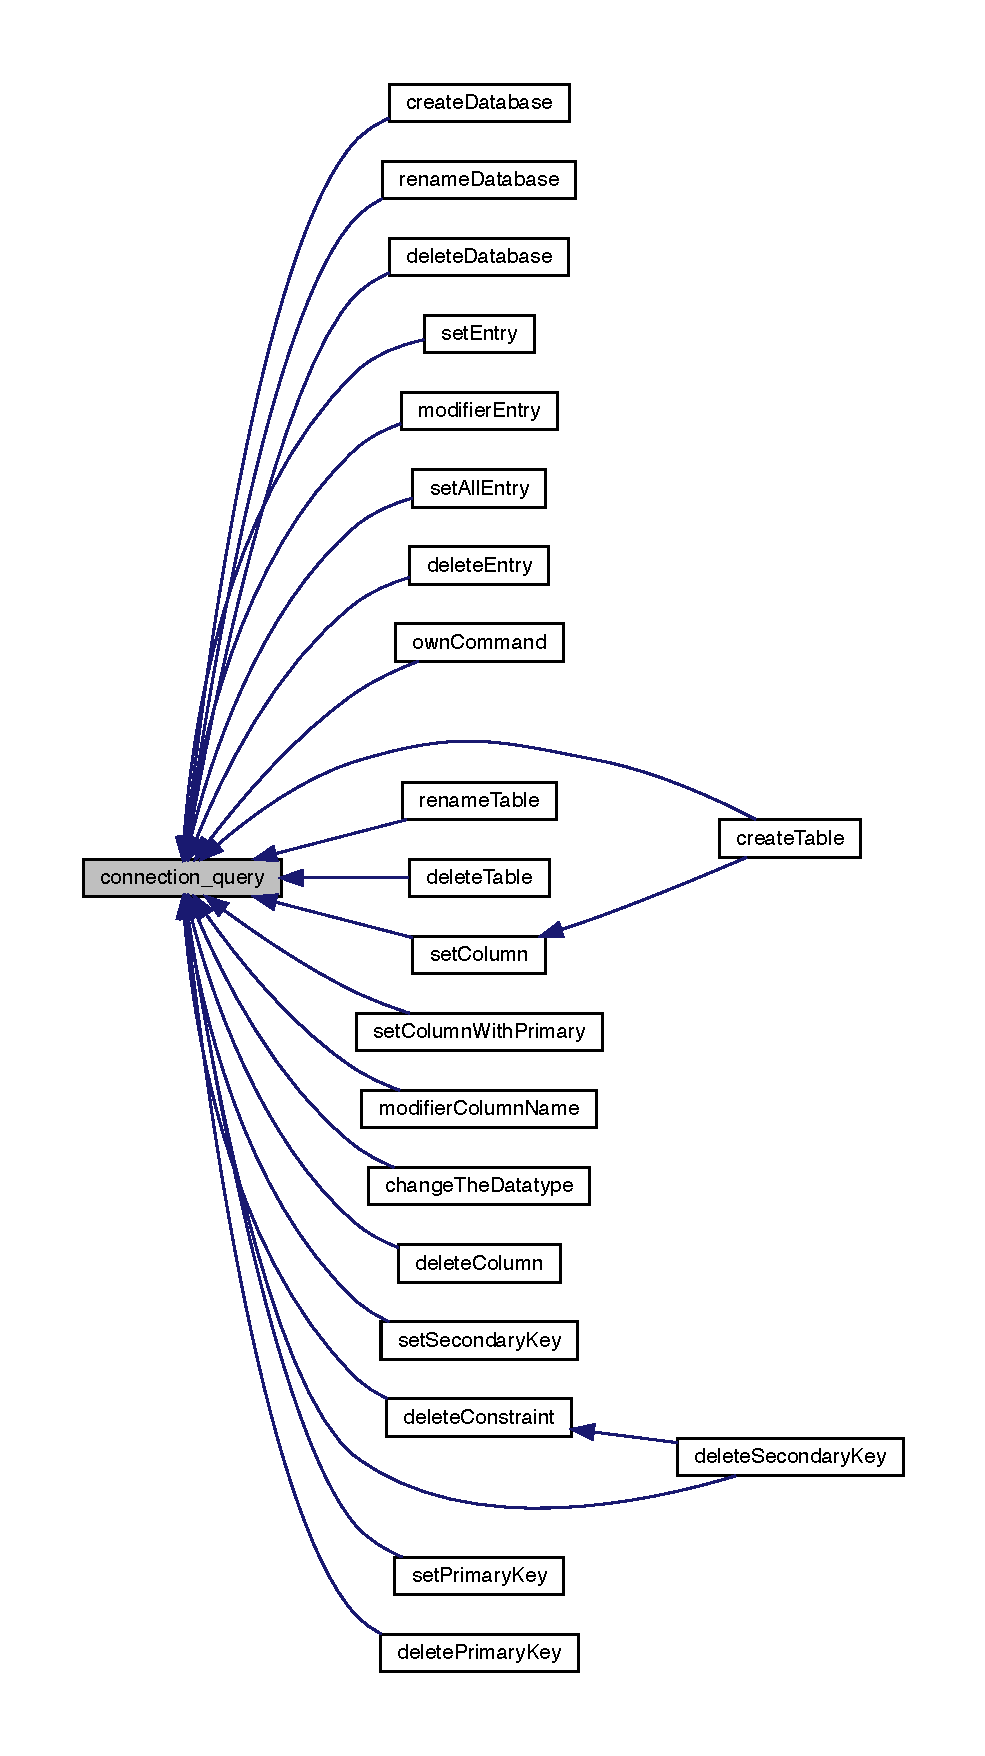
\includegraphics[height=550pt]{connection_8cpp_a6fbdf23f9e84af310b023db3e03bb749_icgraph}
\end{center}
\end{figure}
\mbox{\label{connection_8cpp_a4ec2c49f65ab04fdddbdb7e81e6aab18}} 
\index{connection.\+cpp@{connection.\+cpp}!connectionless@{connectionless}}
\index{connectionless@{connectionless}!connection.\+cpp@{connection.\+cpp}}
\subsubsection{connectionless()}
{\footnotesize\ttfamily bool connectionless (\begin{DoxyParamCaption}\item[{const char}]{host[$\,$],  }\item[{const char}]{user[$\,$],  }\item[{const char}]{passwort[$\,$],  }\item[{const char}]{db[$\,$],  }\item[{unsigned int}]{port,  }\item[{const char $\ast$}]{mac\+O\+S\+\_\+socket,  }\item[{unsigned int}]{client\+\_\+flag }\end{DoxyParamCaption})}



Verbindung zur Datenbank auf einem Server. 

Die Methode \char`\"{}connectionless\char`\"{} wird verwendet, um eine Verbindung zu einer Datenbank mit all ihren nötigen Parametern(z.\+B User,Pw usw.) herzustellen.~\newline
 Um eine Verbindung zu einem lokalen Computer herzustellen, geben Sie \char`\"{}localhost\char`\"{} oder die lokale I\+P-\/\+Adresse für den Server an. ~\newline



\begin{DoxyParams}{Parameter}
{\em host} & = Name des Hosts \\
\hline
{\em user} & = Name des Users \\
\hline
{\em passwort} & = benötigtes Passwort für den Verbindungsaufbau zum S\+Q\+L-\/\+Server \\
\hline
{\em db} & = Name der Datenbank auf die zugegriffen werden soll \\
\hline
{\em port} & = Der zu verwendende Port \\
\hline
{\em socket} & = Der zu verwendende Socket \\
\hline
{\em flag} & = Optional (N\+U\+LL)\\
\hline
\end{DoxyParams}
\begin{DoxyReturn}{Rückgabe}
void 
\end{DoxyReturn}
Hier ist ein Graph, der zeigt, was diese Funktion aufruft\+:
\nopagebreak
\begin{figure}[H]
\begin{center}
\leavevmode
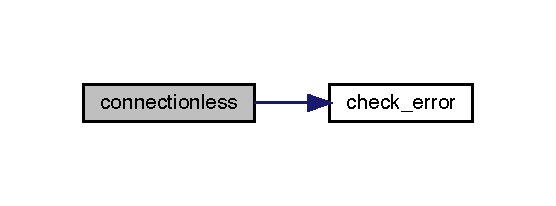
\includegraphics[width=267pt]{connection_8cpp_a4ec2c49f65ab04fdddbdb7e81e6aab18_cgraph}
\end{center}
\end{figure}
\mbox{\label{connection_8cpp_a960705de531a20389fb29928d43258c3}} 
\index{connection.\+cpp@{connection.\+cpp}!disconnect@{disconnect}}
\index{disconnect@{disconnect}!connection.\+cpp@{connection.\+cpp}}
\subsubsection{disconnect()}
{\footnotesize\ttfamily void disconnect (\begin{DoxyParamCaption}{ }\end{DoxyParamCaption})}



Verbindung schließen. 

Die Methode \char`\"{}disconnect\char`\"{} setzt alle ausstehenden Transaktionen zurück. ~\newline
 Anschließend wird die Verbindung zum Verbindungspool freigegeben oder die Verbindung wird geschlossen, wenn das Verbindungspooling deaktiviert ist.~\newline



\begin{DoxyParams}{Parameter}
{\em -\/} & \\
\hline
\end{DoxyParams}
\begin{DoxyReturn}{Rückgabe}
void 
\end{DoxyReturn}


\subsection{Variablen-\/\+Dokumentation}
\mbox{\label{connection_8cpp_a37d24f00a2791852c5c2e3d0acf3845e}} 
\index{connection.\+cpp@{connection.\+cpp}!field@{field}}
\index{field@{field}!connection.\+cpp@{connection.\+cpp}}
\subsubsection{field}
{\footnotesize\ttfamily M\+Y\+S\+Q\+L\+\_\+\+F\+I\+E\+LD$\ast$ field}



Variable für das Aufrufen der Methode mysql\+\_\+fetch\+\_\+field() um Datenbankinformationen ausgeben zu lassen. 

\mbox{\label{connection_8cpp_a801f961b24f1ddf0c1f88a41fd67e764}} 
\index{connection.\+cpp@{connection.\+cpp}!mysql@{mysql}}
\index{mysql@{mysql}!connection.\+cpp@{connection.\+cpp}}
\subsubsection{mysql}
{\footnotesize\ttfamily M\+Y\+S\+QL$\ast$ mysql}



Variable für die Schnittstelle zum S\+Q\+L-\/\+Server. 

\mbox{\label{connection_8cpp_ae6eacc70ad3579c30ba5fb478a363de6}} 
\index{connection.\+cpp@{connection.\+cpp}!result@{result}}
\index{result@{result}!connection.\+cpp@{connection.\+cpp}}
\subsubsection{result}
{\footnotesize\ttfamily M\+Y\+S\+Q\+L\+\_\+\+R\+ES$\ast$ result}



Enthält das Ergebnis einer Abfrage vom S\+Q\+L-\/\+Server. 

\mbox{\label{connection_8cpp_a34269e7c6df16f7d1b6034b9fce28463}} 
\index{connection.\+cpp@{connection.\+cpp}!row@{row}}
\index{row@{row}!connection.\+cpp@{connection.\+cpp}}
\subsubsection{row}
{\footnotesize\ttfamily M\+Y\+S\+Q\+L\+\_\+\+R\+OW row}



Erhält als Ergebnis einer Reihe von einem Result-\/\+Set. 


\section{database.\+cpp-\/\+Dateireferenz}
\label{database_8cpp}\index{database.\+cpp@{database.\+cpp}}
{\ttfamily \#include \char`\"{}database.\+hpp\char`\"{}}\newline
\subsection*{Funktionen}
\begin{DoxyCompactItemize}
\item 
void \textbf{ create\+Database} (std\+::string database\+Name)
\item 
void \textbf{ show\+Databases} ()
\item 
void \textbf{ rename\+Database} (std\+::string database\+Name, std\+::string new\+Database\+Name)
\item 
void \textbf{ delete\+Database} (std\+::string database\+Name)
\end{DoxyCompactItemize}


\subsection{Dokumentation der Funktionen}
\mbox{\label{database_8cpp_abf48eb274e662a7de3f5f190d126b765}} 
\index{database.\+cpp@{database.\+cpp}!create\+Database@{create\+Database}}
\index{create\+Database@{create\+Database}!database.\+cpp@{database.\+cpp}}
\subsubsection{create\+Database()}
{\footnotesize\ttfamily void create\+Database (\begin{DoxyParamCaption}\item[{std\+::string}]{database\+Name }\end{DoxyParamCaption})}

\mbox{\label{database_8cpp_a1d1fac4a7c1506f81908532050a8e58f}} 
\index{database.\+cpp@{database.\+cpp}!delete\+Database@{delete\+Database}}
\index{delete\+Database@{delete\+Database}!database.\+cpp@{database.\+cpp}}
\subsubsection{delete\+Database()}
{\footnotesize\ttfamily void delete\+Database (\begin{DoxyParamCaption}\item[{std\+::string}]{database\+Name }\end{DoxyParamCaption})}

\mbox{\label{database_8cpp_a0659d93a42f84756e52155eb333c4fec}} 
\index{database.\+cpp@{database.\+cpp}!rename\+Database@{rename\+Database}}
\index{rename\+Database@{rename\+Database}!database.\+cpp@{database.\+cpp}}
\subsubsection{rename\+Database()}
{\footnotesize\ttfamily void rename\+Database (\begin{DoxyParamCaption}\item[{std\+::string}]{database\+Name,  }\item[{std\+::string}]{new\+Database\+Name }\end{DoxyParamCaption})}

\mbox{\label{database_8cpp_a812cc82c697df37c6a8a482f85972b4b}} 
\index{database.\+cpp@{database.\+cpp}!show\+Databases@{show\+Databases}}
\index{show\+Databases@{show\+Databases}!database.\+cpp@{database.\+cpp}}
\subsubsection{show\+Databases()}
{\footnotesize\ttfamily void show\+Databases (\begin{DoxyParamCaption}{ }\end{DoxyParamCaption})}


\section{entry.\+cpp-\/\+Dateireferenz}
\label{entry_8cpp}\index{entry.\+cpp@{entry.\+cpp}}
{\ttfamily \#include \char`\"{}entry.\+hpp\char`\"{}}\newline
\subsection*{Funktionen}
\begin{DoxyCompactItemize}
\item 
void \textbf{ set\+Entry} (std\+::string table\+Name, std\+::string column\+Name, std\+::string entry)
\item 
void \textbf{ modifier\+Entry} (std\+::string table\+Name, std\+::string column\+Name, std\+::string old\+Entry, std\+::string new\+Entry)
\item 
void \textbf{ set\+All\+Entry} (std\+::string table\+Name, std\+::vector$<$ std\+::string $>$ \textbf{ row})
\item 
void \textbf{ delete\+Entry} (std\+::string table\+Name, std\+::string column\+Name, std\+::string condition)
\end{DoxyCompactItemize}


\subsection{Dokumentation der Funktionen}
\mbox{\label{entry_8cpp_a1ea4c59c6377c754fd0264b58f476685}} 
\index{entry.\+cpp@{entry.\+cpp}!delete\+Entry@{delete\+Entry}}
\index{delete\+Entry@{delete\+Entry}!entry.\+cpp@{entry.\+cpp}}
\subsubsection{delete\+Entry()}
{\footnotesize\ttfamily void delete\+Entry (\begin{DoxyParamCaption}\item[{std\+::string}]{table\+Name,  }\item[{std\+::string}]{column\+Name,  }\item[{std\+::string}]{condition }\end{DoxyParamCaption})}

\mbox{\label{entry_8cpp_ab254b5514a4950c7479bc4d513c438dc}} 
\index{entry.\+cpp@{entry.\+cpp}!modifier\+Entry@{modifier\+Entry}}
\index{modifier\+Entry@{modifier\+Entry}!entry.\+cpp@{entry.\+cpp}}
\subsubsection{modifier\+Entry()}
{\footnotesize\ttfamily void modifier\+Entry (\begin{DoxyParamCaption}\item[{std\+::string}]{table\+Name,  }\item[{std\+::string}]{column\+Name,  }\item[{std\+::string}]{old\+Entry,  }\item[{std\+::string}]{new\+Entry }\end{DoxyParamCaption})}

\mbox{\label{entry_8cpp_aeb45ccd70b8692b592754a0886c2d109}} 
\index{entry.\+cpp@{entry.\+cpp}!set\+All\+Entry@{set\+All\+Entry}}
\index{set\+All\+Entry@{set\+All\+Entry}!entry.\+cpp@{entry.\+cpp}}
\subsubsection{set\+All\+Entry()}
{\footnotesize\ttfamily void set\+All\+Entry (\begin{DoxyParamCaption}\item[{std\+::string}]{table\+Name,  }\item[{std\+::vector$<$ std\+::string $>$}]{row }\end{DoxyParamCaption})}

\mbox{\label{entry_8cpp_a1faab165d9a7dc43808e1a0075e007f9}} 
\index{entry.\+cpp@{entry.\+cpp}!set\+Entry@{set\+Entry}}
\index{set\+Entry@{set\+Entry}!entry.\+cpp@{entry.\+cpp}}
\subsubsection{set\+Entry()}
{\footnotesize\ttfamily void set\+Entry (\begin{DoxyParamCaption}\item[{std\+::string}]{table\+Name,  }\item[{std\+::string}]{column\+Name,  }\item[{std\+::string}]{entry }\end{DoxyParamCaption})}


\section{main.\+cpp-\/\+Dateireferenz}
\label{main_8cpp}\index{main.\+cpp@{main.\+cpp}}
{\ttfamily \#include \char`\"{}sqllib.\+hpp\char`\"{}}\newline
Include-\/\+Abhängigkeitsdiagramm für main.\+cpp\+:\nopagebreak
\begin{figure}[H]
\begin{center}
\leavevmode
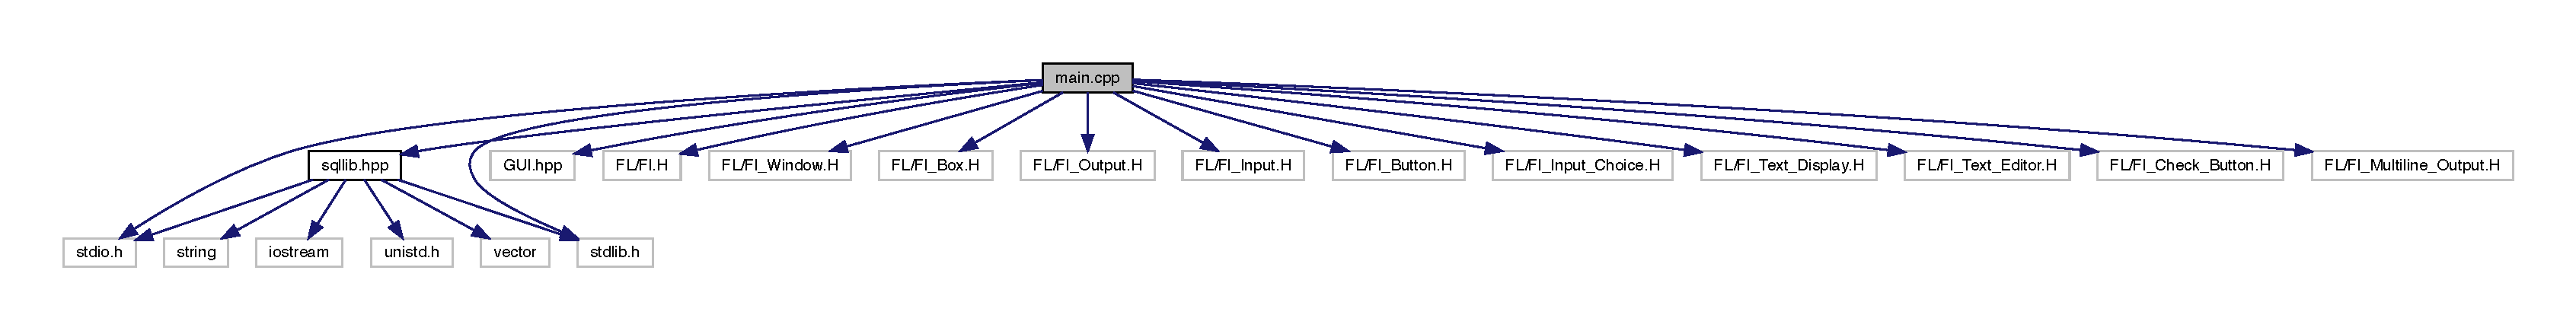
\includegraphics[width=350pt]{main_8cpp__incl}
\end{center}
\end{figure}
\subsection*{Funktionen}
\begin{DoxyCompactItemize}
\item 
int \textbf{ main} (int argc, char $\ast$argv[$\,$])
\end{DoxyCompactItemize}


\subsection{Dokumentation der Funktionen}
\mbox{\label{main_8cpp_a0ddf1224851353fc92bfbff6f499fa97}} 
\index{main.\+cpp@{main.\+cpp}!main@{main}}
\index{main@{main}!main.\+cpp@{main.\+cpp}}
\subsubsection{main()}
{\footnotesize\ttfamily int main (\begin{DoxyParamCaption}\item[{int}]{argc,  }\item[{char $\ast$}]{argv[$\,$] }\end{DoxyParamCaption})}



Definiert in Zeile 4 der Datei main.\+cpp.

Hier ist ein Graph, der zeigt, was diese Funktion aufruft\+:\nopagebreak
\begin{figure}[H]
\begin{center}
\leavevmode
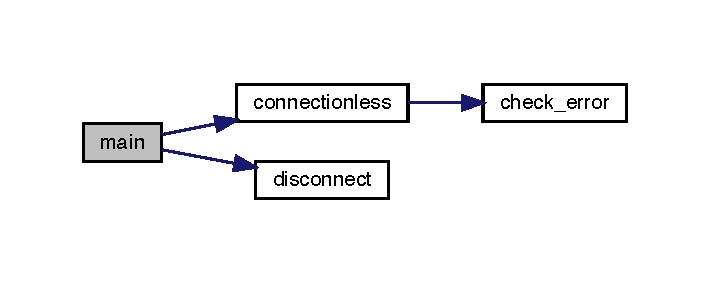
\includegraphics[width=350pt]{main_8cpp_a0ddf1224851353fc92bfbff6f499fa97_cgraph}
\end{center}
\end{figure}

\section{selection\+Request.\+cpp-\/\+Dateireferenz}
\label{selection_request_8cpp}\index{selection\+Request.\+cpp@{selection\+Request.\+cpp}}
{\ttfamily \#include \char`\"{}selection\+Request.\+hpp\char`\"{}}\newline
Include-\/\+Abhängigkeitsdiagramm für selection\+Request.\+cpp\+:\nopagebreak
\begin{figure}[H]
\begin{center}
\leavevmode
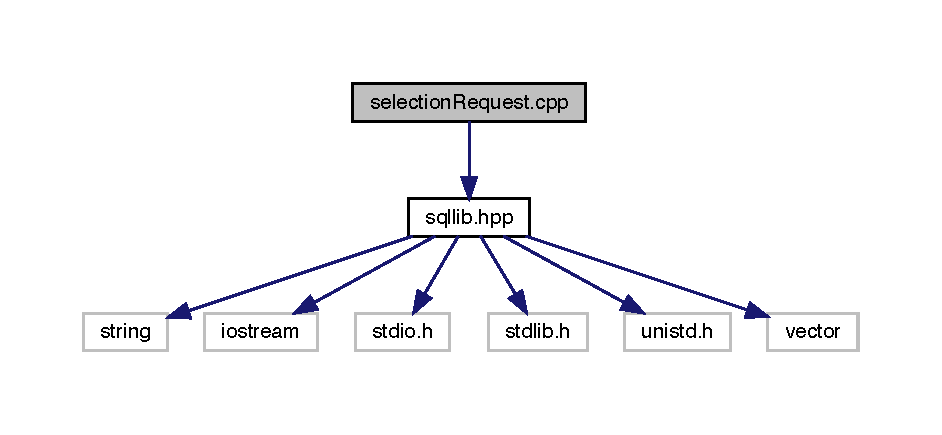
\includegraphics[width=192pt]{selection_request_8cpp__incl}
\end{center}
\end{figure}
\subsection*{Funktionen}
\begin{DoxyCompactItemize}
\item 
void \textbf{ own\+Command} (std\+::string sql\+Command, std\+::string command\+Type)
\begin{DoxyCompactList}\small\item\em Benutzereigener S\+Q\+L-\/\+Befehl. \end{DoxyCompactList}\item 
void \textbf{ select\+Like} (std\+::string table\+Name, std\+::vector$<$ std\+::string $>$columns, std\+::string to\+Search\+Column, std\+::string pattern, std\+::string to\+Search)
\begin{DoxyCompactList}\small\item\em Suche nach Muster. \end{DoxyCompactList}\item 
void \textbf{ select\+Not\+Like} (std\+::string table\+Name, std\+::vector$<$ std\+::string $>$columns, std\+::string to\+Search\+Column, std\+::string pattern, std\+::string to\+Search)
\begin{DoxyCompactList}\small\item\em Suche nach Muster. \end{DoxyCompactList}\item 
void \textbf{ select\+Min\+Or\+Max} (std\+::string table\+Name, std\+::string min\+Or\+Max, std\+::string min\+Or\+Max\+Column, std\+::string alias\+Column)
\begin{DoxyCompactList}\small\item\em Ermittlung des höchsten / niedrigsten Wertes. \end{DoxyCompactList}\item 
void \textbf{ select\+Min\+Or\+Max\+Where} (std\+::string table\+Name, std\+::string min\+Or\+Max, std\+::string min\+Or\+Max\+Column, std\+::string alias\+Column, std\+::string condition\+Column, std\+::string condition\+Value)
\begin{DoxyCompactList}\small\item\em Höchster / niedrigster Wert mit Bedingung und Alias-\/\+Spalte. \end{DoxyCompactList}\item 
void \textbf{ select\+Limit\+Where\+Order\+By} (std\+::string table\+Name, std\+::vector$<$ std\+::string $>$ columns, std\+::string limit\+Number, std\+::string condition\+Column, std\+::string condition\+Value, std\+::string to\+Sort\+Column\+Name, std\+::string sort\+By)
\begin{DoxyCompactList}\small\item\em Bestimmte Anzahl von Datensätzen mit Bedingung abfragen. \end{DoxyCompactList}\item 
void \textbf{ select\+Where\+One\+Column} (std\+::string table\+Name, std\+::string condition\+Column, std\+::string condition\+Value)
\begin{DoxyCompactList}\small\item\em Bestimmte Datensätze von bestimmten Spalten abfragen. \end{DoxyCompactList}\item 
void \textbf{ select\+Where} (std\+::string table\+Name, std\+::vector$<$ std\+::string $>$ columns, std\+::string condition\+Column, std\+::string condition\+Value)
\begin{DoxyCompactList}\small\item\em Anzeigen bestimmter Datensätze mit dem Zusatz der Where-\/\+Clause. \end{DoxyCompactList}\item 
void \textbf{ select\+Bool} (std\+::string table\+Name, std\+::vector$<$ std\+::string $>$ columns, std\+::vector$<$ std\+::string $>$conditions, std\+::vector$<$ std\+::string $>$condition\+Value, std\+::vector$<$ std\+::string $>$ conditions2, std\+::vector$<$ std\+::string $>$condition\+Value2, std\+::vector$<$ std\+::string $>$operators)
\begin{DoxyCompactList}\small\item\em Where-\/\+Clause mit mehreren Bedingungen. \end{DoxyCompactList}\item 
void \textbf{ select\+Where\+Order\+By} (std\+::string table\+Name, std\+::vector$<$ std\+::string $>$ columns, std\+::string condition\+Column, std\+::string condition\+Value, std\+::string to\+Sortcolumn\+Name, std\+::string sort\+By)
\begin{DoxyCompactList}\small\item\em Abfrage von Spalten mit Sortierung. \end{DoxyCompactList}\item 
void \textbf{ select\+Sort\+Table} (std\+::string table\+Name, std\+::string to\+Sort\+Column\+Name, std\+::string sort\+By)
\begin{DoxyCompactList}\small\item\em Tabelle wird nach Angabe sortiert. \end{DoxyCompactList}\item 
void \textbf{ select\+Count} (std\+::string table\+Name, std\+::string count\+Column, std\+::string alias\+Column\+Name)
\begin{DoxyCompactList}\small\item\em Anzahl von ausgewählten Datensätzen. \end{DoxyCompactList}\item 
void \textbf{ select\+Distinct} (std\+::string table\+Name, std\+::vector$<$ std\+::string $>$ columns)
\begin{DoxyCompactList}\small\item\em Redundanzen werden eliminiert und nur einmal angezeigt. \end{DoxyCompactList}\item 
void \textbf{ select\+Count\+Distinct} (std\+::string table\+Name, std\+::string count\+Column)
\begin{DoxyCompactList}\small\item\em Keine Redundanzen / Datensätze werden gezählt. \end{DoxyCompactList}\item 
void \textbf{ select\+Average\+Sum} (std\+::string table\+Name, std\+::string column\+Name)
\begin{DoxyCompactList}\small\item\em Durchschnittswert. \end{DoxyCompactList}\item 
void \textbf{ select\+Sum} (std\+::string table\+Name, std\+::string column\+Name, std\+::string alias\+Column\+Name)
\begin{DoxyCompactList}\small\item\em Summieren von Werten. \end{DoxyCompactList}\item 
void \textbf{ union\+Select} (std\+::vector$<$ std\+::string $>$ table\+Name, std\+::vector$<$ std\+::string $>$ column\+Name)
\begin{DoxyCompactList}\small\item\em Vereinigung zweier Abfragen. \end{DoxyCompactList}\item 
void \textbf{ select\+In} (std\+::string table\+Name, std\+::vector$<$ std\+::string $>$columns, std\+::string search\+In\+Column, std\+::vector$<$ std\+::string $>$condition\+Value)
\begin{DoxyCompactList}\small\item\em Mehrere Abfrageergebnisse bündeln. \end{DoxyCompactList}\item 
void \textbf{ select\+Between} (std\+::string condition\+String, std\+::string condition\+String\+Two, std\+::string table\+Name, std\+::string condition\+Column, std\+::string condition\+Column\+Two, std\+::string condition, std\+::string condition\+Two)
\begin{DoxyCompactList}\small\item\em Eingeschränkte Abfragen. \end{DoxyCompactList}\item 
void \textbf{ select\+Columns\+Alias} (std\+::string table\+Name, std\+::vector$<$ std\+::string $>$columns, std\+::vector$<$ std\+::string $>$aliases)
\begin{DoxyCompactList}\small\item\em Alias-\/\+Spaltennamen. \end{DoxyCompactList}\item 
void \textbf{ select\+Table\+Alias} (std\+::string table\+Name, std\+::vector$<$ std\+::string $>$columns, std\+::string alias\+Table\+Name)
\begin{DoxyCompactList}\small\item\em Zuweisung eines Alias. \end{DoxyCompactList}\item 
void \textbf{ select\+Group\+By} (std\+::string table\+Name, std\+::vector$<$ std\+::string $>$columns, std\+::string condition\+Column, std\+::string condition\+Value, std\+::vector$<$ std\+::string $>$group\+By\+Columns)
\begin{DoxyCompactList}\small\item\em Gruppieren von Ergebnismengen. \end{DoxyCompactList}\item 
void \textbf{ select\+Group\+By\+Order\+By} (std\+::string table\+Name, std\+::vector$<$ std\+::string $>$columns, std\+::string condition\+Column, std\+::string condition\+Value, std\+::vector$<$ std\+::string $>$group\+By\+Columns, std\+::string to\+Sortcolumn\+Name, std\+::string sort\+By)
\begin{DoxyCompactList}\small\item\em Ergebnismengen + sortieren. \end{DoxyCompactList}\item 
void \textbf{ select\+Count\+Group\+By\+Order\+By} (std\+::string table\+Name, std\+::string count\+Column, std\+::vector$<$ std\+::string $>$columns, std\+::string condition\+Column, std\+::string condition\+Value, std\+::vector$<$ std\+::string $>$group\+By\+Columns, std\+::string sort\+By)
\begin{DoxyCompactList}\small\item\em Ergebnismengen gruppieren + zählen der Datensätze + Sortierung. \end{DoxyCompactList}\item 
void \textbf{ select\+Null} (std\+::string table\+Name, std\+::string column\+Name)
\begin{DoxyCompactList}\small\item\em N\+U\+LL Werte. \end{DoxyCompactList}\item 
void \textbf{ select\+Inner\+Join} (std\+::string first\+Table\+Name, std\+::string column\+I\+D\+Table\+One, std\+::vector$<$ std\+::string $>$ columns\+Table\+One, std\+::string second\+Table\+Name, std\+::vector$<$ std\+::string $>$ columns\+Table\+Two)
\begin{DoxyCompactList}\small\item\em Inner\+Join-\/\+Befehl. \end{DoxyCompactList}\item 
void \textbf{ select\+Left\+Join} (std\+::string first\+Table\+Name, std\+::string column\+I\+D\+Table\+One, std\+::vector$<$ std\+::string $>$ columns\+Table\+One, std\+::string second\+Table\+Name, std\+::vector$<$ std\+::string $>$ columns\+Table\+Two)
\begin{DoxyCompactList}\small\item\em Left\+Join Methode. \end{DoxyCompactList}\item 
void \textbf{ select\+Right\+Join} (std\+::string first\+Table\+Name, std\+::string column\+I\+D\+Table\+One, std\+::vector$<$ std\+::string $>$ columns\+Table\+One, std\+::string second\+Table\+Name, std\+::vector$<$ std\+::string $>$ columns\+Table\+Two)
\item 
void \textbf{ select\+Full\+Join} (std\+::string first\+Table\+Name, std\+::string column\+I\+D\+Table\+One, std\+::vector$<$ std\+::string $>$ columns\+Table\+One, std\+::string second\+Table\+Name, std\+::vector$<$ std\+::string $>$ columns\+Table\+Two)
\begin{DoxyCompactList}\small\item\em Full\+Join Methode. \end{DoxyCompactList}\end{DoxyCompactItemize}


\subsection{Dokumentation der Funktionen}
\mbox{\label{selection_request_8cpp_a1909c1b8666cf6e3d31a014c9a9ad2d7}} 
\index{selection\+Request.\+cpp@{selection\+Request.\+cpp}!own\+Command@{own\+Command}}
\index{own\+Command@{own\+Command}!selection\+Request.\+cpp@{selection\+Request.\+cpp}}
\subsubsection{own\+Command()}
{\footnotesize\ttfamily void own\+Command (\begin{DoxyParamCaption}\item[{std\+::string}]{sql\+Command,  }\item[{std\+::string}]{command\+Type }\end{DoxyParamCaption})}



Benutzereigener S\+Q\+L-\/\+Befehl. 

Die Methode \char`\"{}sql\+Command\char`\"{} gibt einen vom Nutzer eingegebenen String(\+S\+Q\+L Befehl) direkt weiter zum S\+QL Server, zu dem wird der Befehlstyp unterschieden. Es wird zwischen 3 Befehlstypen unterschieden\+: Query -\/$>$ simple Abfrage an den S\+QL Server feedback-\/$>$ zeigt den Inhalt einer Spalte an feedback\+All-\/$>$ zeigt die komplette Tabelle mit Spaltenbezeichnugen an


\begin{DoxyParams}{Parameter}
{\em sql\+Command} & = enthält dem vom Nutzer eingegebenen String der später als S\+QL Befehl fungiert \\
\hline
{\em command\+Type} & = enhält dem vom Nutzer gewählten Befehlstyp\\
\hline
\end{DoxyParams}
\begin{DoxyReturn}{Rückgabe}
void
\end{DoxyReturn}
Boolean als return \begin{DoxyAuthor}{Autor}
Martin Meyer 

Steffen Extra 
\end{DoxyAuthor}
Hier ist ein Graph, der zeigt, was diese Funktion aufruft\+:\nopagebreak
\begin{figure}[H]
\begin{center}
\leavevmode
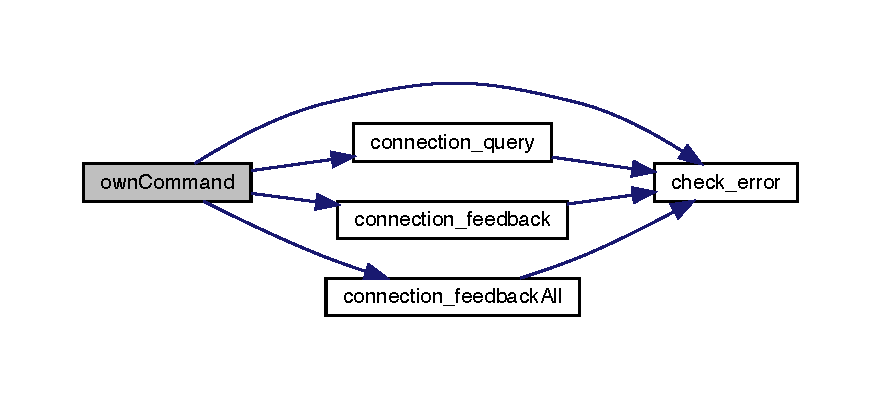
\includegraphics[width=350pt]{selection_request_8cpp_a1909c1b8666cf6e3d31a014c9a9ad2d7_cgraph}
\end{center}
\end{figure}
\mbox{\label{selection_request_8cpp_a01bd0062142a17ad04b7101bac7b38b6}} 
\index{selection\+Request.\+cpp@{selection\+Request.\+cpp}!select\+Average\+Sum@{select\+Average\+Sum}}
\index{select\+Average\+Sum@{select\+Average\+Sum}!selection\+Request.\+cpp@{selection\+Request.\+cpp}}
\subsubsection{select\+Average\+Sum()}
{\footnotesize\ttfamily void select\+Average\+Sum (\begin{DoxyParamCaption}\item[{std\+::string}]{table\+Name,  }\item[{std\+::string}]{column\+Name }\end{DoxyParamCaption})}



Durchschnittswert. 

Die \char`\"{}select\+Average\+Sum\char`\"{} Methode berechnet den Durchschnittswert aller Werte, die in einer Spalte mittels einer Select-\/\+Abfrage ermitteln wurden.~\newline


S\+Q\+L-\/\+Befehl\+: \char`\"{}\+S\+E\+L\+E\+C\+T A\+V\+G(\char`\"{} + column\+Name + \char`\"{}) F\+R\+O\+M \char`\"{} + table\+Name;


\begin{DoxyParams}{Parameter}
{\em table\+Name} & = Name der Tabelle \\
\hline
{\em column\+Name} & = Enthält den Spaltennamen von der, der Durchschnitt berechnet werden soll\\
\hline
\end{DoxyParams}
\begin{DoxyReturn}{Rückgabe}
void
\end{DoxyReturn}
\begin{DoxyAuthor}{Autor}
Martin Meyer 

Steffen Extra 
\end{DoxyAuthor}
Hier ist ein Graph, der zeigt, was diese Funktion aufruft\+:\nopagebreak
\begin{figure}[H]
\begin{center}
\leavevmode
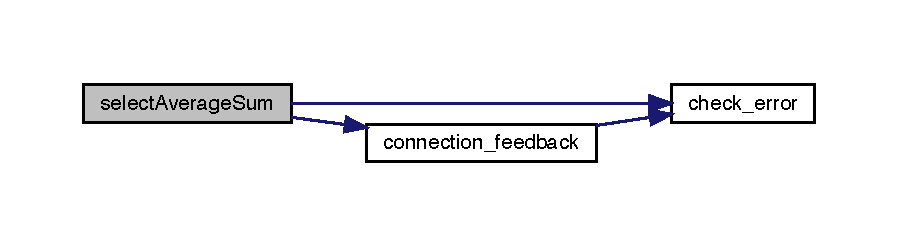
\includegraphics[width=350pt]{selection_request_8cpp_a01bd0062142a17ad04b7101bac7b38b6_cgraph}
\end{center}
\end{figure}
\mbox{\label{selection_request_8cpp_aaa15591ca7a3ba5d40fa77b7ae6753db}} 
\index{selection\+Request.\+cpp@{selection\+Request.\+cpp}!select\+Between@{select\+Between}}
\index{select\+Between@{select\+Between}!selection\+Request.\+cpp@{selection\+Request.\+cpp}}
\subsubsection{select\+Between()}
{\footnotesize\ttfamily void select\+Between (\begin{DoxyParamCaption}\item[{std\+::string}]{condition\+String,  }\item[{std\+::string}]{condition\+String\+Two,  }\item[{std\+::string}]{table\+Name,  }\item[{std\+::string}]{condition\+Column,  }\item[{std\+::string}]{condition\+Column\+Two,  }\item[{std\+::string}]{condition,  }\item[{std\+::string}]{condition\+Two }\end{DoxyParamCaption})}



Eingeschränkte Abfragen. 

Die \char`\"{}select\+Between\char`\"{} Methode beinhält die S\+Q\+L-\/\+Where Bedingungen mit einem eingeschränkten und bestimmten Bereich eines Abfrageergebnisses.~\newline


S\+Q\+L-\/\+Befehl\+: S\+E\+L\+E\+CT $\ast$ \char`\"{} F\+R\+O\+M \char`\"{} + table\+Name + \char`\"{} W\+H\+E\+R\+E \char`\"{} + condition\+Column + \char`\"{} \char`\"{} + condition\+String + \char`\"{} \char`\"{} + condition
\begin{DoxyItemize}
\item \char`\"{} A\+N\+D \char`\"{} + condition\+Column\+Two + \char`\"{} \char`\"{} + condition\+String + \char`\"{} \char`\"{} + condition\+Two;
\end{DoxyItemize}


\begin{DoxyParams}{Parameter}
{\em condition\+String} & = Bedingung (Name = ...) \\
\hline
{\em condition\+String\+Two} & = Bedingung (Name = ...) \\
\hline
{\em tablen\+Name} & = Name der Tabelle \\
\hline
{\em condition\+Column} & = Spalte der ersten Bedingung \\
\hline
{\em condition\+Column2} & = Spalte der zweiten Bedingung \\
\hline
{\em condition} & = Bedingung (... = \textquotesingle{}Hans\textquotesingle{}) \\
\hline
{\em condition\+Two} & = Bedingung (... = \char`\"{}\+Hans\char`\"{})\\
\hline
\end{DoxyParams}
\begin{DoxyReturn}{Rückgabe}
void
\end{DoxyReturn}
\begin{DoxyAuthor}{Autor}
Martin Meyer 

Steffen Extra 
\end{DoxyAuthor}
Hier ist ein Graph, der zeigt, was diese Funktion aufruft\+:\nopagebreak
\begin{figure}[H]
\begin{center}
\leavevmode
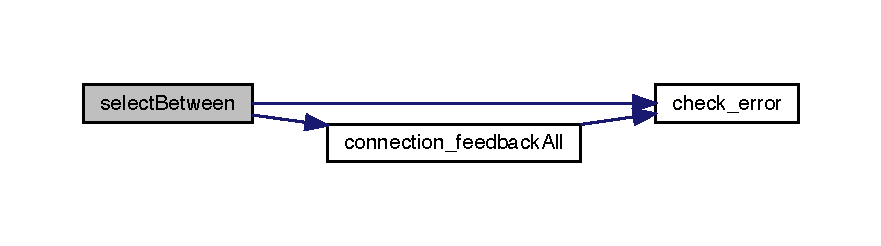
\includegraphics[width=350pt]{selection_request_8cpp_aaa15591ca7a3ba5d40fa77b7ae6753db_cgraph}
\end{center}
\end{figure}
\mbox{\label{selection_request_8cpp_a9ad9be1bbff160a127715440afafb800}} 
\index{selection\+Request.\+cpp@{selection\+Request.\+cpp}!select\+Bool@{select\+Bool}}
\index{select\+Bool@{select\+Bool}!selection\+Request.\+cpp@{selection\+Request.\+cpp}}
\subsubsection{select\+Bool()}
{\footnotesize\ttfamily void select\+Bool (\begin{DoxyParamCaption}\item[{std\+::string}]{table\+Name,  }\item[{std\+::vector$<$ std\+::string $>$}]{columns,  }\item[{std\+::vector$<$ std\+::string $>$}]{conditions,  }\item[{std\+::vector$<$ std\+::string $>$}]{condition\+Value,  }\item[{std\+::vector$<$ std\+::string $>$}]{conditions2,  }\item[{std\+::vector$<$ std\+::string $>$}]{condition\+Value2,  }\item[{std\+::vector$<$ std\+::string $>$}]{operators }\end{DoxyParamCaption})}



Where-\/\+Clause mit mehreren Bedingungen. 

Mithilfe der \char`\"{}select\+Bool\char`\"{} Methode werden die S\+QL Abfragen nur bestimmter Datensätze in einer bestimmten Spalten abgefragt.~\newline
 Zudem kann man ,dank der Funktion mit mehrere Bool-\/\+Bedingungen verknüpfen.~\newline
 Es werden zwei Bedignungsspalten Vektoren, zwei Bedingungswert\+Vektoren sowieo ein Vektor der die Operationen enhält übergeben.~\newline
 Ein Schleifendurchlauf holt sich die zwei Namen der Bedingungsspalten sowie die beiden Bedingungswerte dazu wird dann der boolische Operator hinzugefügt.~\newline
 Die beiden Conditionsvektoren müssen gleich groß sein.~\newline
 Es werden die Spalten angezeigt, die der Nutzer in dem Vektor übergeben hat.~\newline


S\+Q\+L-\/\+Befehl\+: \char`\"{}\+S\+E\+L\+E\+C\+T \char`\"{} + all\+Columns + \char`\"{} F\+R\+O\+M \char`\"{} + table\+Name + \char`\"{} W\+H\+E\+R\+E \char`\"{} + condition\+Operator\+String + \char`\"{};\char`\"{}


\begin{DoxyParams}{Parameter}
{\em table\+Name} & = Name der Tabelle \\
\hline
{\em columns} & = Enthält die Liste der angezeigten Spalten \\
\hline
{\em condition\+Column} & = Enthält den Namen der Bedingungsspalte \\
\hline
{\em condition\+Value} & = Enthält den Bedingungswert \\
\hline
{\em condition\+Column2} & = Enthält den Namen der zweiten zu vergleichnen Bedingungsspalte \\
\hline
{\em condition\+Value2} & = Enthält den zweiten zu vergleichnenen Bedingungswert \\
\hline
{\em operators} & = Enthält die Liste der boolischen Ausdrücke\\
\hline
\end{DoxyParams}
\begin{DoxyReturn}{Rückgabe}
void  Die Funktion gibt ein void zurück -\/$>$ to Do sollte einen Boolean zurückgeben, ob der Befehl erfolgreich bearbeitet wurde.
\end{DoxyReturn}
\begin{DoxyAuthor}{Autor}
Martin Meyer 

Steffen Extra 
\end{DoxyAuthor}
Hier ist ein Graph, der zeigt, was diese Funktion aufruft\+:\nopagebreak
\begin{figure}[H]
\begin{center}
\leavevmode
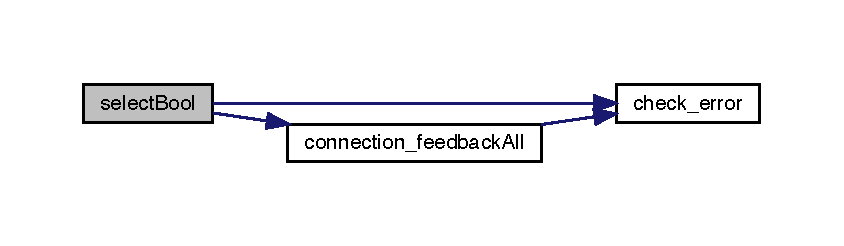
\includegraphics[width=350pt]{selection_request_8cpp_a9ad9be1bbff160a127715440afafb800_cgraph}
\end{center}
\end{figure}
\mbox{\label{selection_request_8cpp_a0bd3f475ec96949ae94bbbbec41f7725}} 
\index{selection\+Request.\+cpp@{selection\+Request.\+cpp}!select\+Columns\+Alias@{select\+Columns\+Alias}}
\index{select\+Columns\+Alias@{select\+Columns\+Alias}!selection\+Request.\+cpp@{selection\+Request.\+cpp}}
\subsubsection{select\+Columns\+Alias()}
{\footnotesize\ttfamily void select\+Columns\+Alias (\begin{DoxyParamCaption}\item[{std\+::string}]{table\+Name,  }\item[{std\+::vector$<$ std\+::string $>$}]{columns,  }\item[{std\+::vector$<$ std\+::string $>$}]{aliases }\end{DoxyParamCaption})}



Alias-\/\+Spaltennamen. 

Die \char`\"{}select\+Columns\+Alias\char`\"{} Methode kann für übergebene Spalte(n) einen ausgwählten Alias-\/\+Spaltenname(n) hinzufügen.~\newline


Zuordnung\+: Spaltenname(i) = Alias-\/\+Spaltennamen(i)~\newline



\begin{DoxyParams}{Parameter}
{\em table\+Name} & = Name der Tabelle \\
\hline
{\em columns} & = Enthält die Liste der zu anzeigenen \& zu unbennenen Spalten \\
\hline
{\em aliases} & = Enthält die Liste mit den Aliasnamen\\
\hline
\end{DoxyParams}
\begin{DoxyReturn}{Rückgabe}
void
\end{DoxyReturn}
\begin{DoxyAuthor}{Autor}
Martin Meyer 

Steffen Extra 
\end{DoxyAuthor}
Hier ist ein Graph, der zeigt, was diese Funktion aufruft\+:\nopagebreak
\begin{figure}[H]
\begin{center}
\leavevmode
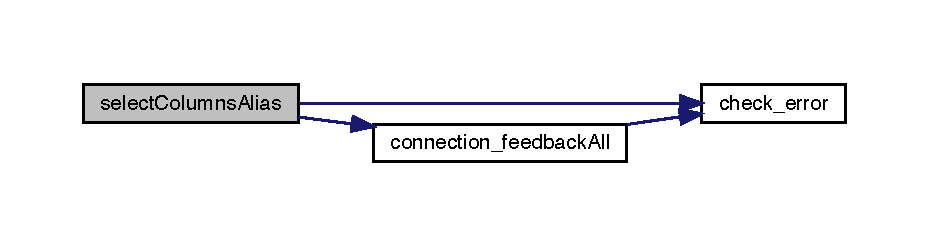
\includegraphics[width=350pt]{selection_request_8cpp_a0bd3f475ec96949ae94bbbbec41f7725_cgraph}
\end{center}
\end{figure}
\mbox{\label{selection_request_8cpp_a00f071477f164f70927ee9923dd77a39}} 
\index{selection\+Request.\+cpp@{selection\+Request.\+cpp}!select\+Count@{select\+Count}}
\index{select\+Count@{select\+Count}!selection\+Request.\+cpp@{selection\+Request.\+cpp}}
\subsubsection{select\+Count()}
{\footnotesize\ttfamily void select\+Count (\begin{DoxyParamCaption}\item[{std\+::string}]{table\+Name,  }\item[{std\+::string}]{count\+Column,  }\item[{std\+::string}]{alias\+Column\+Name }\end{DoxyParamCaption})}



Anzahl von ausgewählten Datensätzen. 

Die select\+Count Methode zählt(\+C\+O\+U\+N\+T) die Anzahl von ausgewählten Datensätzen.~\newline
 Es werden alle Datensätze gezählt, deren Wert nicht N\+U\+LL ist. ~\newline
 Zudem wird die zurück gegebene Spalte mit einem vom Nutzer bestimmten Aliasnamen versehen.~\newline


S\+Q\+L-\/\+Befehl\+: \char`\"{}\+S\+E\+L\+E\+C\+T C\+O\+U\+N\+T(\char`\"{} + count\+Column + \char`\"{}) A\+S \char`\"{} + alias\+Column\+Name + \char`\"{} F\+R\+O\+M \char`\"{} + table\+Name + \char`\"{};\char`\"{}


\begin{DoxyParams}{Parameter}
{\em table\+Name} & = Name der Tabelle \\
\hline
{\em count\+Column} & = Enthält die zu zählende Spalte \\
\hline
{\em alias\+Column} & = Enthält den gewählten Aliasnamen für die zurückgegebene Spalte\\
\hline
\end{DoxyParams}
\begin{DoxyReturn}{Rückgabe}
void
\end{DoxyReturn}
\begin{DoxyAuthor}{Autor}
Martin Meyer 

Steffen Extra 
\end{DoxyAuthor}
Hier ist ein Graph, der zeigt, was diese Funktion aufruft\+:\nopagebreak
\begin{figure}[H]
\begin{center}
\leavevmode
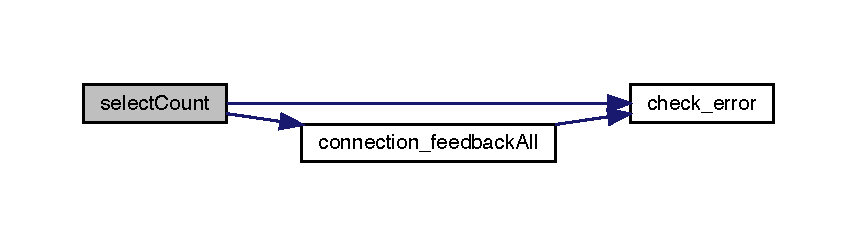
\includegraphics[width=350pt]{selection_request_8cpp_a00f071477f164f70927ee9923dd77a39_cgraph}
\end{center}
\end{figure}
\mbox{\label{selection_request_8cpp_a8d6f770e3b1eb29fce843172c187ccc6}} 
\index{selection\+Request.\+cpp@{selection\+Request.\+cpp}!select\+Count\+Distinct@{select\+Count\+Distinct}}
\index{select\+Count\+Distinct@{select\+Count\+Distinct}!selection\+Request.\+cpp@{selection\+Request.\+cpp}}
\subsubsection{select\+Count\+Distinct()}
{\footnotesize\ttfamily void select\+Count\+Distinct (\begin{DoxyParamCaption}\item[{std\+::string}]{table\+Name,  }\item[{std\+::string}]{count\+Column }\end{DoxyParamCaption})}



Keine Redundanzen / Datensätze werden gezählt. 

Mithilfe der \char`\"{}select\+Count\+Distinct\char`\"{} Methode werden Redundanzen, die in einer Tabellen auftreten können, eliminiert und die Werte werden jeweils nur einmal angezeigt und anschließend werden diese Datensätze gezählt.~\newline


S\+Q\+L-\/\+Befehl\+: \char`\"{}\+S\+E\+L\+E\+C\+T C\+O\+U\+N\+T(\+D\+I\+S\+T\+I\+N\+C\+T \char`\"{} + count\+Column + \char`\"{}) F\+R\+O\+M \char`\"{} + table\+Name + \char`\"{};\char`\"{}


\begin{DoxyParams}{Parameter}
{\em table\+Name} & = Name der Tabelle \\
\hline
{\em count\+Column} & = Enthält die zu zählende Spalte\\
\hline
\end{DoxyParams}
\begin{DoxyReturn}{Rückgabe}
void
\end{DoxyReturn}
\begin{DoxyAuthor}{Autor}
Martin Meyer 

Steffen Extra 
\end{DoxyAuthor}
Hier ist ein Graph, der zeigt, was diese Funktion aufruft\+:\nopagebreak
\begin{figure}[H]
\begin{center}
\leavevmode
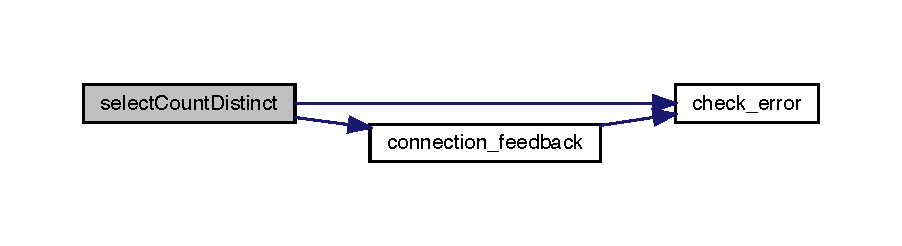
\includegraphics[width=350pt]{selection_request_8cpp_a8d6f770e3b1eb29fce843172c187ccc6_cgraph}
\end{center}
\end{figure}
\mbox{\label{selection_request_8cpp_a851bc3e6b04b4dfaa359b43534a37cd5}} 
\index{selection\+Request.\+cpp@{selection\+Request.\+cpp}!select\+Count\+Group\+By\+Order\+By@{select\+Count\+Group\+By\+Order\+By}}
\index{select\+Count\+Group\+By\+Order\+By@{select\+Count\+Group\+By\+Order\+By}!selection\+Request.\+cpp@{selection\+Request.\+cpp}}
\subsubsection{select\+Count\+Group\+By\+Order\+By()}
{\footnotesize\ttfamily void select\+Count\+Group\+By\+Order\+By (\begin{DoxyParamCaption}\item[{std\+::string}]{table\+Name,  }\item[{std\+::string}]{count\+Column,  }\item[{std\+::vector$<$ std\+::string $>$}]{columns,  }\item[{std\+::string}]{condition\+Column,  }\item[{std\+::string}]{condition\+Value,  }\item[{std\+::vector$<$ std\+::string $>$}]{group\+By\+Columns,  }\item[{std\+::string}]{sort\+By }\end{DoxyParamCaption})}



Ergebnismengen gruppieren + zählen der Datensätze + Sortierung. 

Mithilfe der \char`\"{}select\+Count\+Group\+By\+Order\+By\char`\"{} Methode ist es möglich die Ergebnismenge zu gruppieren. ~\newline
 Das Count zählt die Anzahl der gruppierten Ergebnismengen. Es werden alle Datensätze gezählt, deren Wert nicht N\+U\+LL ist. ~\newline
 Zudem kann der Datensatz anschließend auf-\/ bzw. Absteigend sortiert werden. ~\newline


S\+Q\+L-\/\+Befehl A\+SC\+: std\+::string sql\+Command =\char`\"{}\+S\+E\+L\+E\+C\+T C\+O\+U\+N\+T(\char`\"{} + count\+Column +\char`\"{}),\char`\"{} + all\+Columns + \char`\"{} F\+R\+O\+M \char`\"{} + table\+Name + \char`\"{} W\+H\+E\+R\+E \char`\"{} + condition\+Column + \char`\"{} = \textquotesingle{}\char`\"{} + condition\+Value + \char`\"{}\textquotesingle{} G\+R\+O\+U\+P B\+Y \char`\"{} + all\+Group\+By\+Columns + \char`\"{} O\+R\+D\+E\+R B\+Y C\+O\+U\+N\+T(\char`\"{} + count\+Column +\char`\"{}) A\+S\+C;\char`\"{} S\+Q\+L-\/\+Befehl D\+E\+SC\+: std\+::string sql\+Command =\char`\"{}\+S\+E\+L\+E\+C\+T C\+O\+U\+N\+T(\char`\"{} + count\+Column +\char`\"{}),\char`\"{} + all\+Columns + \char`\"{} F\+R\+O\+M \char`\"{} + table\+Name + \char`\"{} W\+H\+E\+R\+E \char`\"{} + condition\+Column + \char`\"{} = \textquotesingle{}\char`\"{} + condition\+Value + \char`\"{}\textquotesingle{} G\+R\+O\+U\+P B\+Y \char`\"{} + all\+Group\+By\+Columns + \char`\"{} O\+R\+D\+E\+R B\+Y C\+O\+U\+N\+T(\char`\"{} + count\+Column +\char`\"{}) D\+E\+S\+C;\char`\"{}


\begin{DoxyParams}{Parameter}
{\em table\+Name} & = Name der Tabelle , count\+Column = Enthält die zu zählende Spalte \\
\hline
{\em columns} & = Enthält die Liste der zu anzeigenen \& zu unbennenen Spalten \\
\hline
{\em condition\+Column} & = Enthält den Namen der Bedingungsspalte \\
\hline
{\em condition\+Value} & = Enthält den Bedingungswert \\
\hline
{\em group\+By\+Columns} & = Enthält die Liste der zu gruppierenden Spaltennamen \\
\hline
{\em to\+Sort\+Column\+Name} & = Enthält die Spalte zu der sotiert werden soll \\
\hline
{\em Sort\+By} & = Gibt an ob es Aufsteigend bzw Absteigend sotoiert werden soll\\
\hline
\end{DoxyParams}
\begin{DoxyReturn}{Rückgabe}
void
\end{DoxyReturn}
\begin{DoxyAuthor}{Autor}
Martin Meyer 

Steffen Extra 
\end{DoxyAuthor}
Hier ist ein Graph, der zeigt, was diese Funktion aufruft\+:\nopagebreak
\begin{figure}[H]
\begin{center}
\leavevmode
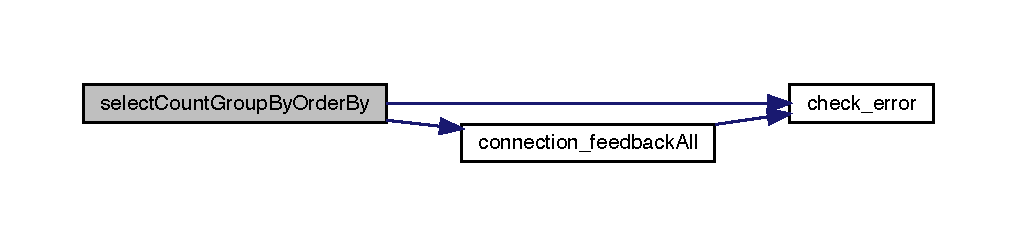
\includegraphics[width=350pt]{selection_request_8cpp_a851bc3e6b04b4dfaa359b43534a37cd5_cgraph}
\end{center}
\end{figure}
\mbox{\label{selection_request_8cpp_aba13caf613af9f91f2a2f1a8f9d49967}} 
\index{selection\+Request.\+cpp@{selection\+Request.\+cpp}!select\+Distinct@{select\+Distinct}}
\index{select\+Distinct@{select\+Distinct}!selection\+Request.\+cpp@{selection\+Request.\+cpp}}
\subsubsection{select\+Distinct()}
{\footnotesize\ttfamily void select\+Distinct (\begin{DoxyParamCaption}\item[{std\+::string}]{table\+Name,  }\item[{std\+::vector$<$ std\+::string $>$}]{columns }\end{DoxyParamCaption})}



Redundanzen werden eliminiert und nur einmal angezeigt. 

Mithilfe der \char`\"{}select\+Distinct\char`\"{} Methode werden Redundanzen, die in einer Tabellen auftreten können, eliminiert und die Werte werden jeweils nur einmal angezeigt.~\newline


S\+Q\+L-\/\+Befehl\+: \char`\"{}\+S\+E\+L\+E\+C\+T D\+I\+S\+T\+I\+N\+C\+T \char`\"{} + all\+Columns + \char`\"{} F\+R\+O\+M \char`\"{} + table\+Name + \char`\"{};\char`\"{}


\begin{DoxyParams}{Parameter}
{\em table\+Name} & = Name der Tabelle \\
\hline
{\em column} & = Enthält die Liste der angezeigten Spalten\\
\hline
\end{DoxyParams}
\begin{DoxyReturn}{Rückgabe}
void
\end{DoxyReturn}
\begin{DoxyAuthor}{Autor}
Martin Meyer 

Steffen Extra 
\end{DoxyAuthor}
Hier ist ein Graph, der zeigt, was diese Funktion aufruft\+:\nopagebreak
\begin{figure}[H]
\begin{center}
\leavevmode
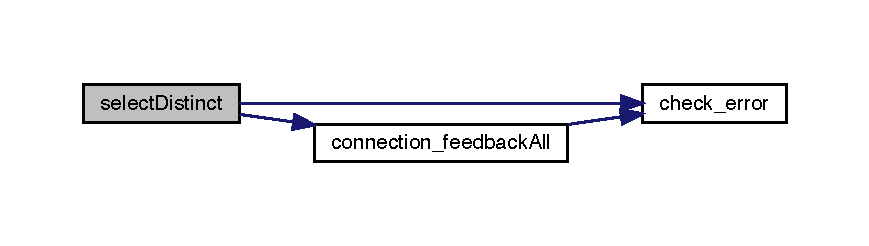
\includegraphics[width=350pt]{selection_request_8cpp_aba13caf613af9f91f2a2f1a8f9d49967_cgraph}
\end{center}
\end{figure}
\mbox{\label{selection_request_8cpp_a41392b97718c999af4867dc0c62ade0c}} 
\index{selection\+Request.\+cpp@{selection\+Request.\+cpp}!select\+Full\+Join@{select\+Full\+Join}}
\index{select\+Full\+Join@{select\+Full\+Join}!selection\+Request.\+cpp@{selection\+Request.\+cpp}}
\subsubsection{select\+Full\+Join()}
{\footnotesize\ttfamily void select\+Full\+Join (\begin{DoxyParamCaption}\item[{std\+::string}]{first\+Table\+Name,  }\item[{std\+::string}]{column\+I\+D\+Table\+One,  }\item[{std\+::vector$<$ std\+::string $>$}]{columns\+Table\+One,  }\item[{std\+::string}]{second\+Table\+Name,  }\item[{std\+::vector$<$ std\+::string $>$}]{columns\+Table\+Two }\end{DoxyParamCaption})}



Full\+Join Methode. 

Mithilfe der \char`\"{}select\+Full\+Join\char`\"{} Methode wird eine neue Ergebnistabelle erstellt.~\newline
 Durch Kombinieren von Spaltenwerten von zwei Tabellen (first\+Table und second\+Table) basierend auf dem Join-\/\+Prädikat.~\newline
 Die Abfrage vergleicht jede Zeile von table1 mit jeder Zeile von table2, um alle Zeilenpaare zu finden, die das Verknüpfungsprädikat erfüllen.~\newline
 Wenn das Join-\/\+Prädikat erfüllt ist, werden Spaltenwerte für jedes übereinstimmende Paar von Zeilen von A und B in einer Ergebniszeile zusammengefasst.~\newline
 Das Schlüsselwort F\+U\+LL O\+U\+T\+ER J\+O\+IN gibt alle Datensätze zurück, wenn eine Übereinstimmung in den Datensätzen der linken (first\+Table) oder der rechten (second\+Table) Tabelle vorliegt.~\newline


S\+Q\+L-\/\+Befehl select $<$\+Auswahl$>$ F\+R\+OM TabelleA F\+U\+LL O\+U\+T\+ER J\+O\+IN TabelleB B ON A.\+ID = B.\+ID


\begin{DoxyParams}{Parameter}
{\em first\+Table\+Name} & = Name der ersten Tabelle \\
\hline
{\em column\+I\+D\+Table\+One} & = Enthält die zu vergleichene Spalte der ersten Tabelle \\
\hline
{\em columns\+Table\+One} & = Enthält die Liste der Spalten die aus der ersten Tabelle angezeigt werden sollen \\
\hline
{\em second\+Table\+Name} & = Name der zweiten Tabelle \\
\hline
{\em columns\+Table\+Two} & = Enthält die Liste der Spalten die aus der zweiten Tabelle angezeigt werden sollen\\
\hline
\end{DoxyParams}
\begin{DoxyReturn}{Rückgabe}
void
\end{DoxyReturn}
\begin{DoxyAuthor}{Autor}
Martin Meyer 

Steffen Extra 
\end{DoxyAuthor}
Hier ist ein Graph, der zeigt, was diese Funktion aufruft\+:\nopagebreak
\begin{figure}[H]
\begin{center}
\leavevmode
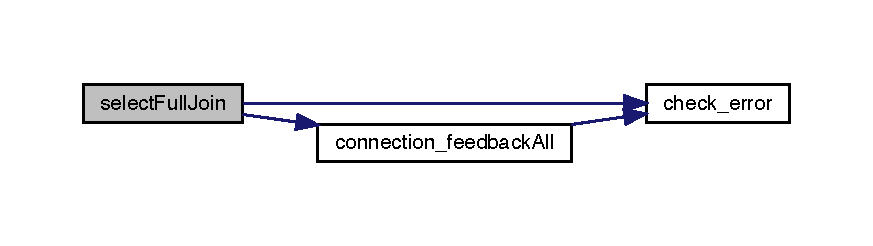
\includegraphics[width=350pt]{selection_request_8cpp_a41392b97718c999af4867dc0c62ade0c_cgraph}
\end{center}
\end{figure}
\mbox{\label{selection_request_8cpp_a54c70afd3e6ad75085ddf6aff29abe87}} 
\index{selection\+Request.\+cpp@{selection\+Request.\+cpp}!select\+Group\+By@{select\+Group\+By}}
\index{select\+Group\+By@{select\+Group\+By}!selection\+Request.\+cpp@{selection\+Request.\+cpp}}
\subsubsection{select\+Group\+By()}
{\footnotesize\ttfamily void select\+Group\+By (\begin{DoxyParamCaption}\item[{std\+::string}]{table\+Name,  }\item[{std\+::vector$<$ std\+::string $>$}]{columns,  }\item[{std\+::string}]{condition\+Column,  }\item[{std\+::string}]{condition\+Value,  }\item[{std\+::vector$<$ std\+::string $>$}]{group\+By\+Columns }\end{DoxyParamCaption})}



Gruppieren von Ergebnismengen. 

Mithilfe der \char`\"{}select\+Group\+By\char`\"{} Methode ist es möglich eine Ergebnismenge zu gruppieren.~\newline


S\+Q\+L-\/\+Befehl\+: \char`\"{}\+S\+E\+L\+E\+C\+T \char`\"{} + all\+Columns + \char`\"{} F\+R\+O\+M \char`\"{} + table\+Name + \char`\"{} W\+H\+E\+R\+E \char`\"{} + condition\+Column + \char`\"{} = \textquotesingle{}\char`\"{} + condition\+Value + \char`\"{}\textquotesingle{} G\+R\+O\+U\+P B\+Y \char`\"{} + all\+Group\+By\+Columns + \char`\"{};\char`\"{}


\begin{DoxyParams}{Parameter}
{\em table\+Name-\/$>$} & Name der Tabelle \\
\hline
{\em columns} & = Enthält die Liste der zu anzeigenen \& zu unbennenen Spalten \\
\hline
{\em condition\+Column} & = Enthält den Namen der Bedingungsspalte \\
\hline
{\em condition\+Value} & = Enthält den Bedingungswert \\
\hline
{\em group\+By\+Columns} & = Enhält die Liste der zu gruppierenden Spaltennamen\\
\hline
\end{DoxyParams}
\begin{DoxyReturn}{Rückgabe}
void
\end{DoxyReturn}
\begin{DoxyAuthor}{Autor}
Martin Meyer 

Steffen Extra 
\end{DoxyAuthor}
Hier ist ein Graph, der zeigt, was diese Funktion aufruft\+:\nopagebreak
\begin{figure}[H]
\begin{center}
\leavevmode
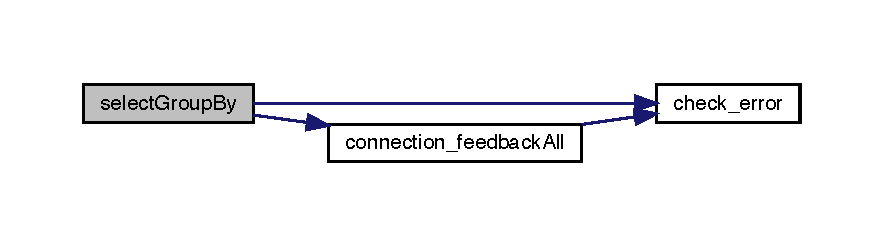
\includegraphics[width=350pt]{selection_request_8cpp_a54c70afd3e6ad75085ddf6aff29abe87_cgraph}
\end{center}
\end{figure}
\mbox{\label{selection_request_8cpp_a5e60ce2e53b91725f89c66539e5bd73d}} 
\index{selection\+Request.\+cpp@{selection\+Request.\+cpp}!select\+Group\+By\+Order\+By@{select\+Group\+By\+Order\+By}}
\index{select\+Group\+By\+Order\+By@{select\+Group\+By\+Order\+By}!selection\+Request.\+cpp@{selection\+Request.\+cpp}}
\subsubsection{select\+Group\+By\+Order\+By()}
{\footnotesize\ttfamily void select\+Group\+By\+Order\+By (\begin{DoxyParamCaption}\item[{std\+::string}]{table\+Name,  }\item[{std\+::vector$<$ std\+::string $>$}]{columns,  }\item[{std\+::string}]{condition\+Column,  }\item[{std\+::string}]{condition\+Value,  }\item[{std\+::vector$<$ std\+::string $>$}]{group\+By\+Columns,  }\item[{std\+::string}]{to\+Sortcolumn\+Name,  }\item[{std\+::string}]{sort\+By }\end{DoxyParamCaption})}



Ergebnismengen + sortieren. 

Mithilfe der \char`\"{}select\+Group\+By\+Order\+By\char`\"{} Methode ist es möglich eine Ergebnismenge zu gruppieren und diese Auf-\/ bzw. Absteigend zu sortieren.~\newline


S\+Q\+L-\/\+Befehl für A\+SC\+: \char`\"{}\+S\+E\+L\+E\+C\+T \char`\"{} + all\+Columns + \char`\"{} F\+R\+O\+M \char`\"{} + table\+Name + \char`\"{} W\+H\+E\+R\+E \char`\"{} + condition\+Column + \char`\"{} = \textquotesingle{}\char`\"{} + condition\+Value + \char`\"{}\textquotesingle{} G\+R\+O\+U\+P B\+Y \char`\"{} + all\+Group\+By\+Columns + \char`\"{} O\+R\+D\+E\+R B\+Y \char`\"{} + to\+Sortcolumn\+Name + \char`\"{} A\+S\+C;\char`\"{}~\newline
 S\+Q\+L-\/\+Befehl für D\+E\+SC\+: \char`\"{}\+S\+E\+L\+E\+C\+T \char`\"{} + all\+Columns + \char`\"{} F\+R\+O\+M \char`\"{} + table\+Name + \char`\"{} W\+H\+E\+R\+E \char`\"{} + condition\+Column + \char`\"{} = \textquotesingle{}\char`\"{} + condition\+Value + \char`\"{}\textquotesingle{} G\+R\+O\+U\+P B\+Y \char`\"{} + all\+Group\+By\+Columns + \char`\"{} O\+R\+D\+E\+R B\+Y \char`\"{} + to\+Sortcolumn\+Name + \char`\"{} D\+E\+S\+C;\char`\"{}~\newline



\begin{DoxyParams}{Parameter}
{\em table\+Name} & = Name der Tabelle \\
\hline
{\em columns} & = Enhält die Liste der zu anzeigenen \& zu unbennenen Spalten \\
\hline
{\em condition\+Column} & = Enthält den Namen der Bedingungsspalte \\
\hline
{\em condition\+Value} & = Enthält den Bedingungswert \\
\hline
{\em group\+By\+Columns} & = Enthält die Liste der zu gruppierenden Spaltennamen \\
\hline
{\em to\+Sort\+Column\+Name} & = Enthält die Spalte zu der sotiert werden soll \\
\hline
{\em Sort\+By} & = Gibt an ob es Aufsteigend bzw Absteigend sotoiert werden soll\\
\hline
\end{DoxyParams}
\begin{DoxyReturn}{Rückgabe}
void
\end{DoxyReturn}
\begin{DoxyAuthor}{Autor}
Martin Meyer 

Steffen Extra 
\end{DoxyAuthor}
Hier ist ein Graph, der zeigt, was diese Funktion aufruft\+:\nopagebreak
\begin{figure}[H]
\begin{center}
\leavevmode
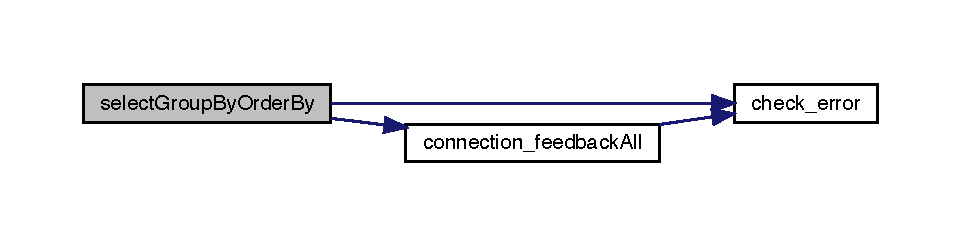
\includegraphics[width=350pt]{selection_request_8cpp_a5e60ce2e53b91725f89c66539e5bd73d_cgraph}
\end{center}
\end{figure}
\mbox{\label{selection_request_8cpp_ac3a0a9620e1b5ac8c90104b1daea4f5f}} 
\index{selection\+Request.\+cpp@{selection\+Request.\+cpp}!select\+In@{select\+In}}
\index{select\+In@{select\+In}!selection\+Request.\+cpp@{selection\+Request.\+cpp}}
\subsubsection{select\+In()}
{\footnotesize\ttfamily void select\+In (\begin{DoxyParamCaption}\item[{std\+::string}]{table\+Name,  }\item[{std\+::vector$<$ std\+::string $>$}]{columns,  }\item[{std\+::string}]{search\+In\+Column,  }\item[{std\+::vector$<$ std\+::string $>$}]{condition\+Value }\end{DoxyParamCaption})}



Mehrere Abfrageergebnisse bündeln. 

Die \char`\"{}select\+In\char`\"{} Methode kann mehrere Abfrageergebnisse in einer S\+Q\+L-\/\+Anweisung zu bündeln.~\newline
 Damit kann der IN Operator leicht mehrere OR Operatoren ersetzen und vereinfacht damit die Struktur von komplexen O\+R-\/\+Bedingungen.~\newline


S\+Q\+L-\/\+Befehl\+: \char`\"{}\+S\+E\+L\+E\+C\+T \char`\"{} + all\+Columns + \char`\"{} F\+R\+O\+M \char`\"{} + table\+Name + \char`\"{} W\+H\+E\+R\+E \char`\"{} + search\+In\+Column + \char`\"{} I\+N \char`\"{} + \char`\"{} (\char`\"{} + comparativ\+Values + \char`\"{});\char`\"{}


\begin{DoxyParams}{Parameter}
{\em table\+Name} & = Name der Tabelle \\
\hline
{\em columns} & = Enthält die Liste der angezeigten Spalten \\
\hline
{\em search\+In\+Column} & = Enthält den Spaltennamen in der die Werte vergleicht werden \\
\hline
{\em condition\+Value} & = Enthält eine Liste der zu vergleichenden Werten\\
\hline
\end{DoxyParams}
\begin{DoxyReturn}{Rückgabe}
void
\end{DoxyReturn}
\begin{DoxyAuthor}{Autor}
Martin Meyer 

Steffen Extra 
\end{DoxyAuthor}
Hier ist ein Graph, der zeigt, was diese Funktion aufruft\+:\nopagebreak
\begin{figure}[H]
\begin{center}
\leavevmode
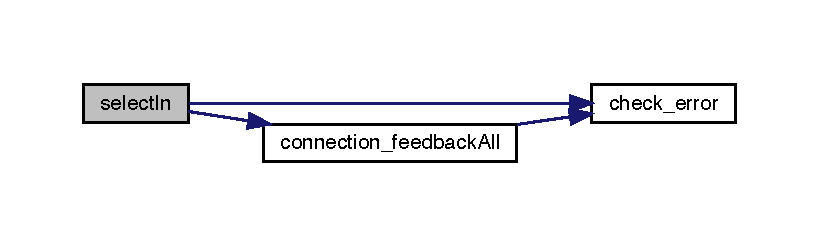
\includegraphics[width=350pt]{selection_request_8cpp_ac3a0a9620e1b5ac8c90104b1daea4f5f_cgraph}
\end{center}
\end{figure}
\mbox{\label{selection_request_8cpp_aa0d6684a1d4f8e82d699b713e38c9d44}} 
\index{selection\+Request.\+cpp@{selection\+Request.\+cpp}!select\+Inner\+Join@{select\+Inner\+Join}}
\index{select\+Inner\+Join@{select\+Inner\+Join}!selection\+Request.\+cpp@{selection\+Request.\+cpp}}
\subsubsection{select\+Inner\+Join()}
{\footnotesize\ttfamily void select\+Inner\+Join (\begin{DoxyParamCaption}\item[{std\+::string}]{first\+Table\+Name,  }\item[{std\+::string}]{column\+I\+D\+Table\+One,  }\item[{std\+::vector$<$ std\+::string $>$}]{columns\+Table\+One,  }\item[{std\+::string}]{second\+Table\+Name,  }\item[{std\+::vector$<$ std\+::string $>$}]{columns\+Table\+Two }\end{DoxyParamCaption})}



Inner\+Join-\/\+Befehl. 

Mithilfe der \char`\"{}select\+Inner\+Join\char`\"{} Methode wird eine neue Ergebnistabelle erstellt.~\newline
 Durch Kombinieren von Spaltenwerten zweier Tabellen (first\+Table und second\+Table) basierend auf dem Join-\/\+Prädikat.~\newline
 Die Abfrage vergleicht jede Zeile von table1 mit jeder Zeile von table2 um alle Zeilenpaare zu finden, die das Verknüpfungsprädikat erfüllen.~\newline
 Wenn das Join-\/\+Prädikat erfüllt ist, werden Spaltenwerte für jedes übereinstimmende Paar Zeilen von A und B in einer Ergebniszeile zusammengefasst.~\newline
 Das Schlüsselwort I\+N\+N\+ER J\+O\+IN wählt Datensätze mit übereinstimmenden Werten in beiden Tabellen aus.~\newline


S\+Q\+L-\/\+Befehl\+: select $<$\+Auswahl$>$ F\+R\+OM TabelleA I\+N\+N\+ER J\+O\+IN TabelleB B ON A.\+ID = B.\+ID


\begin{DoxyParams}{Parameter}
{\em first\+Table\+Name} & = Name der ersten Tabelle \\
\hline
{\em column\+I\+D\+Table\+One} & = Enthält die zu vergleichene Spalte der ersten Tabelle \\
\hline
{\em columns\+Table\+One} & = Enthält die Liste der Spalten die aus der ersten Tabelle angezeigt werden sollen \\
\hline
{\em second\+Table\+Name} & = Enthält den Tabellennamen der zweiten Tabelle \\
\hline
{\em columns\+Table\+Two} & = Enthält die Liste der Spalten die aus der zweiten Tabelle angezeigt werden sollen\\
\hline
\end{DoxyParams}
\begin{DoxyReturn}{Rückgabe}
void
\end{DoxyReturn}
\begin{DoxyAuthor}{Autor}
Martin Meyer 

Steffen Extra 
\end{DoxyAuthor}
Hier ist ein Graph, der zeigt, was diese Funktion aufruft\+:\nopagebreak
\begin{figure}[H]
\begin{center}
\leavevmode
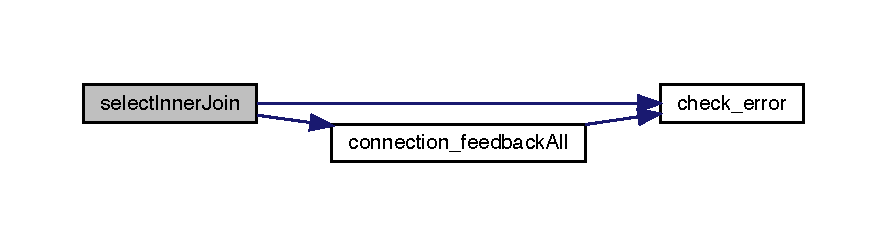
\includegraphics[width=350pt]{selection_request_8cpp_aa0d6684a1d4f8e82d699b713e38c9d44_cgraph}
\end{center}
\end{figure}
\mbox{\label{selection_request_8cpp_a85d81ccc1d4c2b8cb7edcfe0a5a585f5}} 
\index{selection\+Request.\+cpp@{selection\+Request.\+cpp}!select\+Left\+Join@{select\+Left\+Join}}
\index{select\+Left\+Join@{select\+Left\+Join}!selection\+Request.\+cpp@{selection\+Request.\+cpp}}
\subsubsection{select\+Left\+Join()}
{\footnotesize\ttfamily void select\+Left\+Join (\begin{DoxyParamCaption}\item[{std\+::string}]{first\+Table\+Name,  }\item[{std\+::string}]{column\+I\+D\+Table\+One,  }\item[{std\+::vector$<$ std\+::string $>$}]{columns\+Table\+One,  }\item[{std\+::string}]{second\+Table\+Name,  }\item[{std\+::vector$<$ std\+::string $>$}]{columns\+Table\+Two }\end{DoxyParamCaption})}



Left\+Join Methode. 

Mithilfe der \char`\"{}select\+Left\+Join\char`\"{} Methode wird eine neue Ergebnistabelle erstellt.~\newline
 Durch Kombinieren von Spaltenwerten von zwei Tabellen (first\+Table und second\+Table) basierend auf dem Join-\/\+Prädikat.~\newline
 Die Abfrage vergleicht jede Zeile von table1 mit jeder Zeile von table2, um alle Zeilenpaare zu finden, die das Verknüpfungsprädikat erfüllen.~\newline
 Wenn das Join-\/\+Prädikat erfüllt ist, werden Spaltenwerte für jedes übereinstimmende Paar von Zeilen von A und B in einer Ergebniszeile zusammengefasst.~\newline
 Das Schlüsselwort L\+E\+FT J\+O\+IN gibt alle Datensätze der linken Tabelle (first\+Table) und die übereinstimmenden Datensätze der rechten Tabelle (second\+Table) zurück.~\newline
 Das Ergebnis ist N\+U\+LL von rechts, wenn keine Übereinstimmung vorliegt.~\newline


S\+Q\+L-\/\+Befehl\+: select $<$\+Auswahl$>$ F\+R\+OM TabelleA L\+E\+FT J\+O\+IN TabelleB B ON A.\+ID = B.\+ID


\begin{DoxyParams}{Parameter}
{\em first\+Table\+Name} & = Name der ersten Tabelle \\
\hline
{\em column\+I\+D\+Table\+One} & = Enthält die zu vergleichene Spalte der ersten Tabelle \\
\hline
{\em columns\+Table\+One} & = Enthält die Liste der Spalten die aus der ersten Tabelle angezeigt werden sollen \\
\hline
{\em second\+Table\+Name} & =Enthält den Tabellennamen der zweiten Tabelle \\
\hline
{\em columns\+Table\+Two} & = Enthält die Liste der Spalten die aus der zweiten Tabelle angezeigt werden sollen\\
\hline
\end{DoxyParams}
\begin{DoxyReturn}{Rückgabe}
void
\end{DoxyReturn}
\begin{DoxyAuthor}{Autor}
Martin Meyer 

Steffen Extra 
\end{DoxyAuthor}
Hier ist ein Graph, der zeigt, was diese Funktion aufruft\+:\nopagebreak
\begin{figure}[H]
\begin{center}
\leavevmode
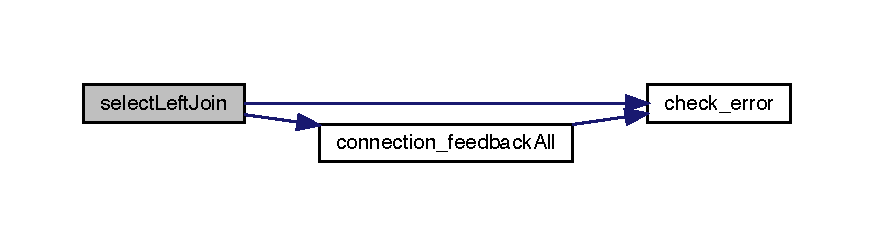
\includegraphics[width=350pt]{selection_request_8cpp_a85d81ccc1d4c2b8cb7edcfe0a5a585f5_cgraph}
\end{center}
\end{figure}
\mbox{\label{selection_request_8cpp_a80ced4bb0e929e97740616c59374d992}} 
\index{selection\+Request.\+cpp@{selection\+Request.\+cpp}!select\+Like@{select\+Like}}
\index{select\+Like@{select\+Like}!selection\+Request.\+cpp@{selection\+Request.\+cpp}}
\subsubsection{select\+Like()}
{\footnotesize\ttfamily void select\+Like (\begin{DoxyParamCaption}\item[{std\+::string}]{table\+Name,  }\item[{std\+::vector$<$ std\+::string $>$}]{columns,  }\item[{std\+::string}]{to\+Search\+Column,  }\item[{std\+::string}]{pattern,  }\item[{std\+::string}]{to\+Search }\end{DoxyParamCaption})}



Suche nach Muster. 

Die Methode \char`\"{}select\+Like\char`\"{} ermöglicht eine Suche auf der Grundlage eines vorher definierten regulären Musters.~\newline
 Muster\+: Findet einen Datzensatz der z.\+B mit einem \char`\"{}a\char`\"{} beginnt.~\newline
 Findet einen Datzensatz der z.\+B mit einem \char`\"{}a\char`\"{} endet.~\newline
 Findet einen Datensatz der z.\+b ein \char`\"{}or\char`\"{} an beliebiger Positon enhält. ~\newline
 Findet einen Datensatz der z.\+B ein \char`\"{}r\char`\"{} an der zweiten Position enthält.~\newline
 Findet einen Datensatz der z.\+B mit einem \char`\"{}a\char`\"{} beginnt und einem O anfängt. ~\newline
 -\/$>$(Bedingung nur bei zwei Buchstaben erfüllt -\/$>$ Fehlermeldung bei mehr als zwei Buchstaben)~\newline


S\+Q\+L-\/\+Befehl\+: \char`\"{}\+S\+E\+L\+E\+C\+T \char`\"{} + all\+Columns + \char`\"{} F\+R\+O\+M \char`\"{} + table\+Name + \char`\"{} W\+H\+E\+R\+E \char`\"{} + to\+Search\+Column + \char`\"{}  L\+I\+K\+E \char`\"{} + \char`\"{}\textquotesingle{}\char`\"{} + to\+Search + \char`\"{}\%\textquotesingle{};\char`\"{}


\begin{DoxyParams}{Parameter}
{\em table\+Name} & = Name der Tabelle \\
\hline
{\em columns} & = Enhält die Liste der angezeigten Spalten \\
\hline
{\em to\+Search\+Column} & = Enhält die zu suchende Spalte \\
\hline
{\em pattern} & = enhält das ausgewählte Muster \\
\hline
{\em to\+Search} & = enhält das zu suchende Element\\
\hline
\end{DoxyParams}
\begin{DoxyReturn}{Rückgabe}
void  Boolean als Rückgabewert
\end{DoxyReturn}
\begin{DoxyAuthor}{Autor}
Martin Meyer 

Steffen Extra 
\end{DoxyAuthor}
Hier ist ein Graph, der zeigt, was diese Funktion aufruft\+:\nopagebreak
\begin{figure}[H]
\begin{center}
\leavevmode
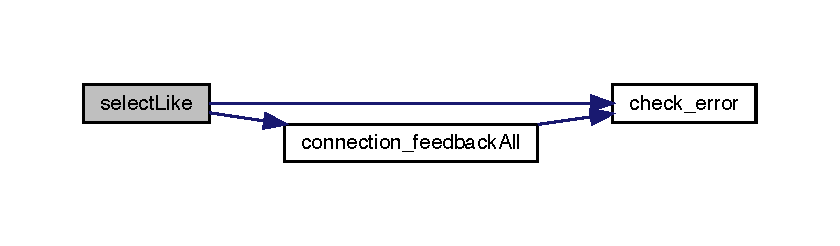
\includegraphics[width=350pt]{selection_request_8cpp_a80ced4bb0e929e97740616c59374d992_cgraph}
\end{center}
\end{figure}
\mbox{\label{selection_request_8cpp_a94c57cf58c1b2812e3d1ce9b3837286d}} 
\index{selection\+Request.\+cpp@{selection\+Request.\+cpp}!select\+Limit\+Where\+Order\+By@{select\+Limit\+Where\+Order\+By}}
\index{select\+Limit\+Where\+Order\+By@{select\+Limit\+Where\+Order\+By}!selection\+Request.\+cpp@{selection\+Request.\+cpp}}
\subsubsection{select\+Limit\+Where\+Order\+By()}
{\footnotesize\ttfamily void select\+Limit\+Where\+Order\+By (\begin{DoxyParamCaption}\item[{std\+::string}]{table\+Name,  }\item[{std\+::vector$<$ std\+::string $>$}]{columns,  }\item[{std\+::string}]{limit\+Number,  }\item[{std\+::string}]{condition\+Column,  }\item[{std\+::string}]{condition\+Value,  }\item[{std\+::string}]{to\+Sort\+Column\+Name,  }\item[{std\+::string}]{sort\+By }\end{DoxyParamCaption})}



Bestimmte Anzahl von Datensätzen mit Bedingung abfragen. 

Die Methode \char`\"{}select\+Limit\+Where\char`\"{} dient dazu eine vom Nutzer festgelegte Anzahl an Datensätzen abzufragen, verknüpft mit einer Bedingungs Klausel. ~\newline
 Zudem wird es Aufsteigend bzw. Absteigend sotiert.~\newline


S\+Q\+L-\/\+Befehl A\+SC\+: \char`\"{}\+S\+E\+L\+E\+C\+T \char`\"{} + all\+Columns + \char`\"{} F\+R\+O\+M \char`\"{} + table\+Name + \char`\"{} W\+H\+E\+R\+E \char`\"{} + condition\+Column + \char`\"{} = \textquotesingle{}\char`\"{} + condition\+Value + \char`\"{}\textquotesingle{}\char`\"{} + \char`\"{}  O\+R\+D\+E\+R B\+Y \char`\"{} + to\+Sortcolumn\+Name + \char`\"{} A\+S\+C \char`\"{} + \char`\"{} L\+I\+M\+I\+T \char`\"{} + limit\+Number + \char`\"{};\char`\"{}; S\+Q\+L-\/\+Befehl D\+E\+SC\+: \char`\"{}\+S\+E\+L\+E\+C\+T \char`\"{} + all\+Columns + \char`\"{} F\+R\+O\+M \char`\"{} + table\+Name + \char`\"{} W\+H\+E\+R\+E \char`\"{} + condition\+Column + \char`\"{} = \textquotesingle{}\char`\"{} + condition\+Value + \char`\"{}\textquotesingle{}\char`\"{} + \char`\"{}  O\+R\+D\+E\+R B\+Y \char`\"{} + to\+Sort\+Column\+Name + \char`\"{} D\+E\+S\+C \char`\"{} + \char`\"{} L\+I\+M\+I\+T \char`\"{} + limit\+Number + \char`\"{};\char`\"{};


\begin{DoxyParams}{Parameter}
{\em table\+Name} & = Name der Tabelle \\
\hline
{\em columns} & = Enthält die Liste der angezeigten Spalten \\
\hline
{\em limit\+Number} & = Anzahl der angezeigten Datensätze \\
\hline
{\em condition\+Column} & = Enhält den Namen der Bedingungsspalte \\
\hline
{\em condition\+Value} & = Enhält den Bedigungswert \\
\hline
{\em to\+Sort\+Column\+Name} & = Enhält die Spalte zu der sotiert werden soll \\
\hline
{\em Sort\+By} & =Gibt an ob es Aufsteigend bzw Absteigend sotoiert werden soll\\
\hline
\end{DoxyParams}
\begin{DoxyReturn}{Rückgabe}
void  Die Funktion gibt ein void zurück -\/$>$ to Do sollte einen Boolean zurückgeben, ob der Befehl erfolgreich bearbeitet wurde.
\end{DoxyReturn}
\begin{DoxyAuthor}{Autor}
Martin Meyer 

Steffen Extra 
\end{DoxyAuthor}
Hier ist ein Graph, der zeigt, was diese Funktion aufruft\+:\nopagebreak
\begin{figure}[H]
\begin{center}
\leavevmode
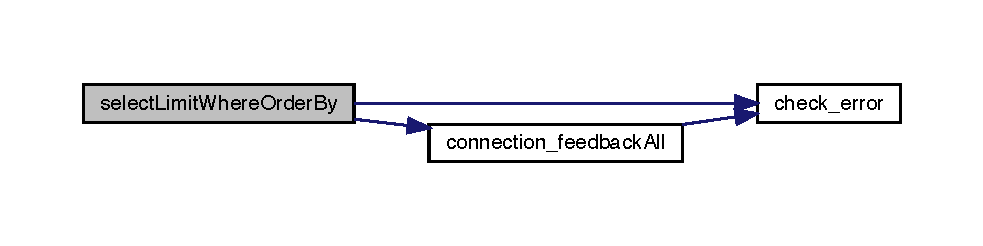
\includegraphics[width=350pt]{selection_request_8cpp_a94c57cf58c1b2812e3d1ce9b3837286d_cgraph}
\end{center}
\end{figure}
\mbox{\label{selection_request_8cpp_ae4c9217024bfe521a229e0b4162e5ef7}} 
\index{selection\+Request.\+cpp@{selection\+Request.\+cpp}!select\+Min\+Or\+Max@{select\+Min\+Or\+Max}}
\index{select\+Min\+Or\+Max@{select\+Min\+Or\+Max}!selection\+Request.\+cpp@{selection\+Request.\+cpp}}
\subsubsection{select\+Min\+Or\+Max()}
{\footnotesize\ttfamily void select\+Min\+Or\+Max (\begin{DoxyParamCaption}\item[{std\+::string}]{table\+Name,  }\item[{std\+::string}]{min\+Or\+Max,  }\item[{std\+::string}]{min\+Or\+Max\+Column,  }\item[{std\+::string}]{alias\+Column }\end{DoxyParamCaption})}



Ermittlung des höchsten / niedrigsten Wertes. 

Die Methode \char`\"{}select\+Min\+Or\+Max\char`\"{} ermittelt den höchsten bzw. niedrigsten Wert einer Tabellenspalte und liefert die Spalte mit einem Aliasnamen zurück.~\newline


S\+Q\+L-\/\+Befehl für das Minimum\+: \char`\"{}\+S\+E\+L\+E\+C\+T M\+I\+N(\char`\"{} + min\+Or\+Max\+Column +\char`\"{})\char`\"{} + \char`\"{} A\+S \char`\"{} + alias\+Column + \char`\"{} F\+R\+O\+M \char`\"{} + table\+Name + \char`\"{};\char`\"{} S\+Q\+L-\/\+Befehl für das Maximum\+: \char`\"{}\+S\+E\+L\+E\+C\+T M\+A\+X(\char`\"{} + min\+Or\+Max\+Column +\char`\"{})\char`\"{} + \char`\"{} A\+S \char`\"{} + alias\+Column + \char`\"{} F\+R\+O\+M \char`\"{} + table\+Name + \char`\"{};\char`\"{}


\begin{DoxyParams}{Parameter}
{\em table\+Name} & = Name der Tabelle \\
\hline
{\em min\+Or\+Max} & = Gibt an welcher Befehl ausgeführt werden soll. \\
\hline
{\em min\+Or\+Max\+Column} & = Gibt die Spalte an, die den Min/\+Max Wert enthalten soll \\
\hline
{\em as\+Column} & = Enhält den gewählten Aliasnamen für die Min/\+Max Spalte\\
\hline
\end{DoxyParams}
\begin{DoxyReturn}{Rückgabe}
void  Boolean als Rückgabewert
\end{DoxyReturn}
\begin{DoxyAuthor}{Autor}
Martin Meyer 

Steffen Extra 
\end{DoxyAuthor}
Hier ist ein Graph, der zeigt, was diese Funktion aufruft\+:\nopagebreak
\begin{figure}[H]
\begin{center}
\leavevmode
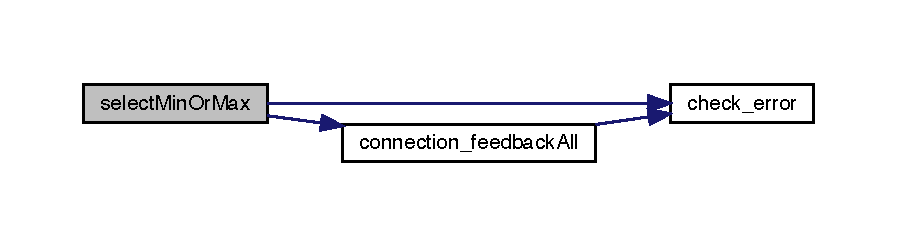
\includegraphics[width=350pt]{selection_request_8cpp_ae4c9217024bfe521a229e0b4162e5ef7_cgraph}
\end{center}
\end{figure}
\mbox{\label{selection_request_8cpp_a39f437d3c3c841e8a82b9ad1b514007e}} 
\index{selection\+Request.\+cpp@{selection\+Request.\+cpp}!select\+Min\+Or\+Max\+Where@{select\+Min\+Or\+Max\+Where}}
\index{select\+Min\+Or\+Max\+Where@{select\+Min\+Or\+Max\+Where}!selection\+Request.\+cpp@{selection\+Request.\+cpp}}
\subsubsection{select\+Min\+Or\+Max\+Where()}
{\footnotesize\ttfamily void select\+Min\+Or\+Max\+Where (\begin{DoxyParamCaption}\item[{std\+::string}]{table\+Name,  }\item[{std\+::string}]{min\+Or\+Max,  }\item[{std\+::string}]{min\+Or\+Max\+Column,  }\item[{std\+::string}]{alias\+Column,  }\item[{std\+::string}]{condition\+Column,  }\item[{std\+::string}]{condition\+Value }\end{DoxyParamCaption})}



Höchster / niedrigster Wert mit Bedingung und Alias-\/\+Spalte. 

Die Methode \char`\"{}select\+Min\+Or\+Max\+Where\char`\"{} ermittelt den höchsten bzw. niedrigsten Wert einer Tabellenspalte verknüpft mit einer Bedigungs Klausel und liefert die Alias-\/\+Spalte zurück.~\newline


S\+Q\+L-\/\+Befehl für das Minimum = \char`\"{}\+S\+E\+L\+E\+C\+T M\+I\+N(\char`\"{} + min\+Or\+Max\+Column +\char`\"{})\char`\"{} +\char`\"{} A\+S \char`\"{} + alias\+Column + \char`\"{} F\+R\+O\+M \char`\"{} + table\+Name + \char`\"{} W\+H\+E\+R\+E \char`\"{} + condition\+Column + \char`\"{} = \textquotesingle{}\char`\"{} + condition\+Value + \char`\"{}\textquotesingle{}\char`\"{} + \char`\"{};\char`\"{}~\newline
 S\+Q\+L-\/\+Befehl für das Maximum = \char`\"{}\+S\+E\+L\+E\+C\+T M\+A\+X(\char`\"{} + min\+Or\+Max\+Column +\char`\"{})\char`\"{} +\char`\"{} A\+S \char`\"{} + alias\+Column + \char`\"{} F\+R\+O\+M \char`\"{} + table\+Name + \char`\"{} W\+H\+E\+R\+E \char`\"{} + condition\+Column + \char`\"{} = \textquotesingle{}\char`\"{} + condition\+Value + \char`\"{}\textquotesingle{}\char`\"{} + \char`\"{};\char`\"{}


\begin{DoxyParams}{Parameter}
{\em table\+Name} & = Enhält den Tabellennamen \\
\hline
{\em min\+Or\+Max} & = Gibt an welcher Befehl ausgeführt werden soll. \\
\hline
{\em min\+Or\+Max\+Column} & = Gibt die Spalte an, die den Min/\+Max Wert enthalten soll \\
\hline
{\em alias\+Column} & = Enhält den gewählten Aliasnamen für die Min/\+Max Spalte \\
\hline
{\em condition\+Column} & = Enhält den Namen der Bedingungsspalte \\
\hline
{\em condition\+Value} & = Enhält den Bedigungswert\\
\hline
\end{DoxyParams}
\begin{DoxyReturn}{Rückgabe}
void  Boolean als Rückgabewert
\end{DoxyReturn}
\begin{DoxyAuthor}{Autor}
Martin Meyer 

Steffen Extra 
\end{DoxyAuthor}
Hier ist ein Graph, der zeigt, was diese Funktion aufruft\+:\nopagebreak
\begin{figure}[H]
\begin{center}
\leavevmode
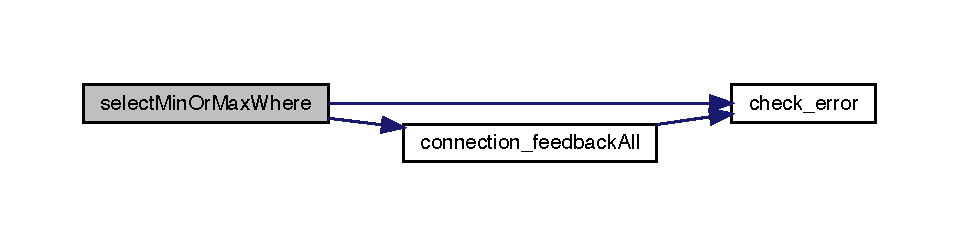
\includegraphics[width=350pt]{selection_request_8cpp_a39f437d3c3c841e8a82b9ad1b514007e_cgraph}
\end{center}
\end{figure}
\mbox{\label{selection_request_8cpp_aab8b32ae4ac6aeddc5c05578b4c79ace}} 
\index{selection\+Request.\+cpp@{selection\+Request.\+cpp}!select\+Not\+Like@{select\+Not\+Like}}
\index{select\+Not\+Like@{select\+Not\+Like}!selection\+Request.\+cpp@{selection\+Request.\+cpp}}
\subsubsection{select\+Not\+Like()}
{\footnotesize\ttfamily void select\+Not\+Like (\begin{DoxyParamCaption}\item[{std\+::string}]{table\+Name,  }\item[{std\+::vector$<$ std\+::string $>$}]{columns,  }\item[{std\+::string}]{to\+Search\+Column,  }\item[{std\+::string}]{pattern,  }\item[{std\+::string}]{to\+Search }\end{DoxyParamCaption})}



Suche nach Muster. 

Die Methode \char`\"{}select\+Not\+Like\char`\"{} ermöglicht eine Suche auf der Grundlage eines vorher definierten regulären Musters.~\newline
 Muster\+: Findet einen Datzensatz der z.\+B nicht mit einem \char`\"{}a\char`\"{} beginnt.~\newline
 Findet einen Datzensatz der z.\+B nicht mit einem \char`\"{}a\char`\"{} endet.~\newline
 Findet einen Datensatz der z.\+b nicht ein \char`\"{}or\char`\"{} an beliebiger Positon enhält. ~\newline
 Findet einen Datensatz der z.\+B nicht ein \char`\"{}r\char`\"{} an der zweiten Position enthält.~\newline
 Findet einen Datensatz der z.\+B nicht mit einem \char`\"{}a\char`\"{} beginnt und einem O anfängt.~\newline
 -\/$>$(Bedingung nur bei zwei Buchstaben erfüllt -\/$>$ Fehlermeldung bei mehr als zwei Buchstaben)~\newline


S\+Q\+L-\/\+Befehl\+:


\begin{DoxyParams}{Parameter}
{\em table\+Name} & = Name der Tabelle \\
\hline
{\em columns} & = Enthält die Liste der angezeigten Spalten \\
\hline
{\em to\+Search\+Column} & = Enthält die zu suchende Spalte \\
\hline
{\em pattern} & = enhält das ausgewählte Muster \\
\hline
{\em to\+Search} & = enhält das zu suchende Element\\
\hline
\end{DoxyParams}
\begin{DoxyReturn}{Rückgabe}
void  Boolean als Rückgabewert
\end{DoxyReturn}
\begin{DoxyAuthor}{Autor}
Martin Meyer 

Steffen Extra 
\end{DoxyAuthor}
Hier ist ein Graph, der zeigt, was diese Funktion aufruft\+:\nopagebreak
\begin{figure}[H]
\begin{center}
\leavevmode
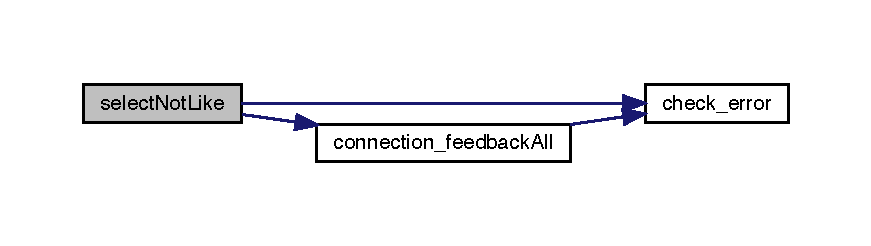
\includegraphics[width=350pt]{selection_request_8cpp_aab8b32ae4ac6aeddc5c05578b4c79ace_cgraph}
\end{center}
\end{figure}
\mbox{\label{selection_request_8cpp_aedcd1503abb6715de26a92d34714dcce}} 
\index{selection\+Request.\+cpp@{selection\+Request.\+cpp}!select\+Null@{select\+Null}}
\index{select\+Null@{select\+Null}!selection\+Request.\+cpp@{selection\+Request.\+cpp}}
\subsubsection{select\+Null()}
{\footnotesize\ttfamily void select\+Null (\begin{DoxyParamCaption}\item[{std\+::string}]{table\+Name,  }\item[{std\+::string}]{column\+Name }\end{DoxyParamCaption})}



N\+U\+LL Werte. 

Die select\+Null Methode prüft eine Spalte auf den Wert N\+U\+LL.~\newline


S\+Q\+L-\/\+Befehl\+: \char`\"{}\+S\+E\+L\+E\+C\+T $\ast$ \char`\"{} + \char`\"{} F\+R\+O\+M \char`\"{} + table\+Name + \char`\"{} W\+H\+E\+R\+E \char`\"{} + column\+Name + \char`\"{} I\+S N\+U\+L\+L\char`\"{} + \char`\"{} O\+R \textquotesingle{} \textquotesingle{}; \char`\"{}


\begin{DoxyParams}{Parameter}
{\em table\+Name} & = Name der Tabelle \\
\hline
{\em Column\+Name} & = Enhält den Namen der Bedingungsspalte\\
\hline
\end{DoxyParams}
\begin{DoxyReturn}{Rückgabe}
void
\end{DoxyReturn}
\begin{DoxyAuthor}{Autor}
Martin Meyer 

Steffen Extra 
\end{DoxyAuthor}
Hier ist ein Graph, der zeigt, was diese Funktion aufruft\+:\nopagebreak
\begin{figure}[H]
\begin{center}
\leavevmode
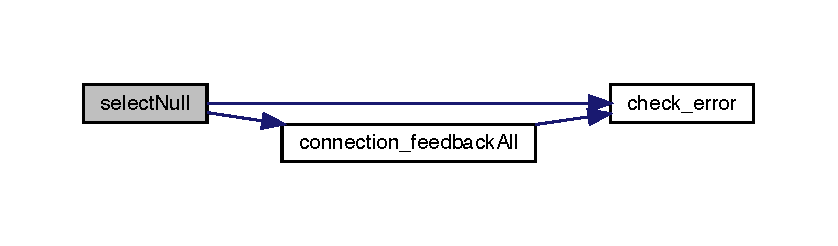
\includegraphics[width=350pt]{selection_request_8cpp_aedcd1503abb6715de26a92d34714dcce_cgraph}
\end{center}
\end{figure}
\mbox{\label{selection_request_8cpp_aff2cca0ae3f40a8b3ec70e85702bb8fc}} 
\index{selection\+Request.\+cpp@{selection\+Request.\+cpp}!select\+Right\+Join@{select\+Right\+Join}}
\index{select\+Right\+Join@{select\+Right\+Join}!selection\+Request.\+cpp@{selection\+Request.\+cpp}}
\subsubsection{select\+Right\+Join()}
{\footnotesize\ttfamily void select\+Right\+Join (\begin{DoxyParamCaption}\item[{std\+::string}]{first\+Table\+Name,  }\item[{std\+::string}]{column\+I\+D\+Table\+One,  }\item[{std\+::vector$<$ std\+::string $>$}]{columns\+Table\+One,  }\item[{std\+::string}]{second\+Table\+Name,  }\item[{std\+::vector$<$ std\+::string $>$}]{columns\+Table\+Two }\end{DoxyParamCaption})}

Mithilfe der \char`\"{}select\+Right\+Join\char`\"{} Methode wird eine neue Ergebnistabelle erstellt.~\newline
 Durch Kombinieren von Spaltenwerten von zwei Tabellen (first\+Table und second\+Table) basierend auf dem Join-\/\+Prädikat. ~\newline
 Die Abfrage vergleicht jede Zeile von table1 mit jeder Zeile von table2, um alle Zeilenpaare zu finden, die das Verknüpfungsprädikat erfüllen. ~\newline
 Wenn das Join-\/\+Prädikat erfüllt ist, werden Spaltenwerte für jedes übereinstimmende Paar von Zeilen von A und B in einer Ergebniszeile zusammengefasst.~\newline
 Das Schlüsselwort R\+I\+G\+HT J\+O\+IN gibt alle Datensätze der rechten Tabelle (second\+Table) und die übereinstimmenden Datensätze der linken Tabelle (first\+Table) zurück. ~\newline
 Das Ergebnis ist N\+U\+LL von links, wenn keine Übereinstimmung vorliegt.~\newline


S\+Q\+L-\/\+Befehl\+: select $<$\+Auswahl$>$ F\+R\+OM TabelleA L\+E\+FT J\+O\+IN TabelleB B ON A.\+ID = B.\+ID


\begin{DoxyParams}{Parameter}
{\em first\+Table\+Name} & = Name der ersten Tabelle  = Enthält die zu vergleichene Spalte der ersten Tabelle \\
\hline
{\em columns\+Table\+One} & = Enthält die Liste der Spalten die aus der ersten Tabelle angezeigt werden sollen \\
\hline
{\em second\+Table\+Name} & = Name der zweiten Tabelle \\
\hline
{\em columns\+Table\+Two} & = Enthält die Liste der Spalten die aus der zweiten Tabelle angezeigt werden sollen\\
\hline
\end{DoxyParams}
\begin{DoxyReturn}{Rückgabe}
void
\end{DoxyReturn}
\begin{DoxyAuthor}{Autor}
Martin Meyer 

Steffen Extra 
\end{DoxyAuthor}
Hier ist ein Graph, der zeigt, was diese Funktion aufruft\+:\nopagebreak
\begin{figure}[H]
\begin{center}
\leavevmode
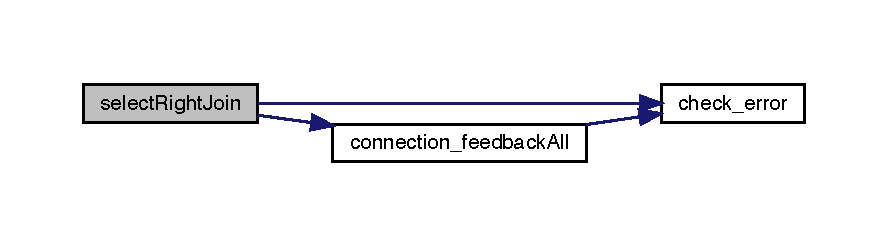
\includegraphics[width=350pt]{selection_request_8cpp_aff2cca0ae3f40a8b3ec70e85702bb8fc_cgraph}
\end{center}
\end{figure}
\mbox{\label{selection_request_8cpp_a6a41ec41130fdce3f2c4dd701438f26a}} 
\index{selection\+Request.\+cpp@{selection\+Request.\+cpp}!select\+Sort\+Table@{select\+Sort\+Table}}
\index{select\+Sort\+Table@{select\+Sort\+Table}!selection\+Request.\+cpp@{selection\+Request.\+cpp}}
\subsubsection{select\+Sort\+Table()}
{\footnotesize\ttfamily void select\+Sort\+Table (\begin{DoxyParamCaption}\item[{std\+::string}]{table\+Name,  }\item[{std\+::string}]{to\+Sort\+Column\+Name,  }\item[{std\+::string}]{sort\+By }\end{DoxyParamCaption})}



Tabelle wird nach Angabe sortiert. 

Mithilfe der \char`\"{}select\+Sort\+Table\char`\"{} Methode wird eine angebene Tabelle nach einer angebenen Spalte auf-\/ bzw. -\/\+Absteigend sortiert.~\newline
 Die ganze Tabelle wird ausgebenen.~\newline


S\+Q\+L-\/\+Befehl für A\+SC = \char`\"{}\+S\+E\+L\+E\+C\+T $\ast$ F\+R\+O\+M \char`\"{} + table\+Name + \char`\"{} O\+R\+D\+E\+R B\+Y \char`\"{} + to\+Sort\+Column\+Name + \char`\"{} A\+S\+C;\char`\"{} S\+Q\+L-\/\+Befehl für D\+E\+SC = \char`\"{}\+S\+E\+L\+E\+C\+T $\ast$ F\+R\+O\+M \char`\"{} + table\+Name + \char`\"{} O\+R\+D\+E\+R B\+Y \char`\"{} + to\+Sort\+Column\+Name + \char`\"{} D\+E\+S\+C;\char`\"{}


\begin{DoxyParams}{Parameter}
{\em table\+Name} & = Name der Tabelle \\
\hline
{\em to\+Sort\+Column\+Name} & = Enhält die Spalte zu der sotiert werden soll \\
\hline
{\em Sort\+By} & = Gibt an ob es Aufsteigend bzw Absteigend sotoiert werden soll\\
\hline
\end{DoxyParams}
\begin{DoxyReturn}{Rückgabe}
void
\end{DoxyReturn}
\begin{DoxyAuthor}{Autor}
Martin Meyer 

Steffen Extra 
\end{DoxyAuthor}
Hier ist ein Graph, der zeigt, was diese Funktion aufruft\+:\nopagebreak
\begin{figure}[H]
\begin{center}
\leavevmode
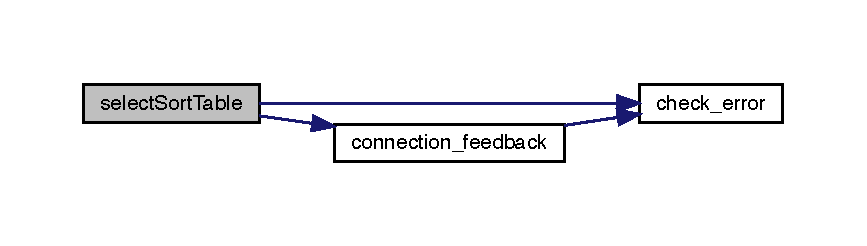
\includegraphics[width=350pt]{selection_request_8cpp_a6a41ec41130fdce3f2c4dd701438f26a_cgraph}
\end{center}
\end{figure}
\mbox{\label{selection_request_8cpp_a9f37b58ba921dc5e6b5d4a5d0fefe28e}} 
\index{selection\+Request.\+cpp@{selection\+Request.\+cpp}!select\+Sum@{select\+Sum}}
\index{select\+Sum@{select\+Sum}!selection\+Request.\+cpp@{selection\+Request.\+cpp}}
\subsubsection{select\+Sum()}
{\footnotesize\ttfamily void select\+Sum (\begin{DoxyParamCaption}\item[{std\+::string}]{table\+Name,  }\item[{std\+::string}]{column\+Name,  }\item[{std\+::string}]{alias\+Column\+Name }\end{DoxyParamCaption})}



Summieren von Werten. 

Die \char`\"{}select\+Sum\char`\"{} Methode summiert die Werte einer Tabellenspalte und liefert sie zurück.~\newline
 Zudem wird die zurück gegebene Spalte mit einem vom Nutzer bestimmten Aliasnamen versehen.~\newline


S\+Q\+L-\/\+Befehl\+: \char`\"{}\+S\+E\+L\+E\+C\+T S\+U\+M(\char`\"{} + column\+Name + \char`\"{}) A\+S \char`\"{} + alias\+Column\+Name+ \char`\"{} F\+R\+O\+M \char`\"{} + table\+Name;


\begin{DoxyParams}{Parameter}
{\em table\+Name} & = Name der Tabelle \\
\hline
{\em column\+Name} & = Enthält den Spaltennamen von der, die Summe berechnet werden soll \\
\hline
{\em alias\+Column\+Name} & = Enthält den Aliasnamen\\
\hline
\end{DoxyParams}
\begin{DoxyReturn}{Rückgabe}
void
\end{DoxyReturn}
\begin{DoxyAuthor}{Autor}
Martin Meyer 

Steffen Extra 
\end{DoxyAuthor}
Hier ist ein Graph, der zeigt, was diese Funktion aufruft\+:\nopagebreak
\begin{figure}[H]
\begin{center}
\leavevmode
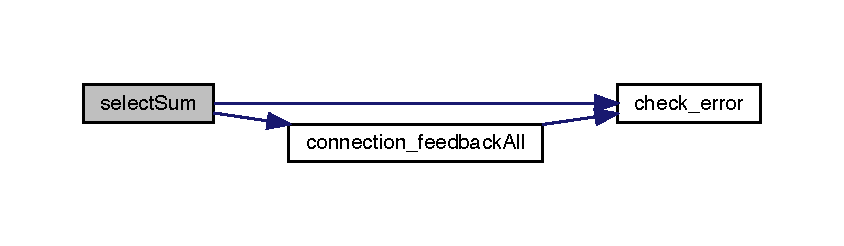
\includegraphics[width=350pt]{selection_request_8cpp_a9f37b58ba921dc5e6b5d4a5d0fefe28e_cgraph}
\end{center}
\end{figure}
\mbox{\label{selection_request_8cpp_a3ac5ebbcfb624dc5178315c85c4b15fa}} 
\index{selection\+Request.\+cpp@{selection\+Request.\+cpp}!select\+Table\+Alias@{select\+Table\+Alias}}
\index{select\+Table\+Alias@{select\+Table\+Alias}!selection\+Request.\+cpp@{selection\+Request.\+cpp}}
\subsubsection{select\+Table\+Alias()}
{\footnotesize\ttfamily void select\+Table\+Alias (\begin{DoxyParamCaption}\item[{std\+::string}]{table\+Name,  }\item[{std\+::vector$<$ std\+::string $>$}]{columns,  }\item[{std\+::string}]{alias\+Table\+Name }\end{DoxyParamCaption})}



Zuweisung eines Alias. 

Die \char`\"{}select\+Table\+Alias\char`\"{} Methode kann der übergebenen Tabelle einen Alias-\/\+Tabellennamen zuweisen.

S\+Q\+L-\/\+Befehl\+: \char`\"{}\+S\+E\+L\+E\+C\+T \char`\"{} + column\+Alias + \char`\"{} F\+R\+O\+M \char`\"{} + table\+Name + \char`\"{} A\+S \char`\"{} + alias\+Table\+Name +\char`\"{};\char`\"{}


\begin{DoxyParams}{Parameter}
{\em table\+Name} & = Name der Tabelle \\
\hline
{\em columns} & = Enthält die Liste der zu anzeigenen Spalten \\
\hline
{\em alias\+Tabellennamen} & = Enthält den Alias-\/\+Tabellennamen\\
\hline
\end{DoxyParams}
\begin{DoxyReturn}{Rückgabe}
void
\end{DoxyReturn}
\begin{DoxyAuthor}{Autor}
Martin Meyer 

Steffen Extra 
\end{DoxyAuthor}
Hier ist ein Graph, der zeigt, was diese Funktion aufruft\+:\nopagebreak
\begin{figure}[H]
\begin{center}
\leavevmode
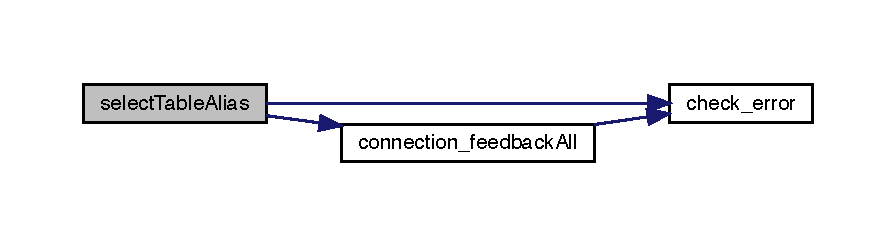
\includegraphics[width=350pt]{selection_request_8cpp_a3ac5ebbcfb624dc5178315c85c4b15fa_cgraph}
\end{center}
\end{figure}
\mbox{\label{selection_request_8cpp_a90eb635de3f1856a45557b42f18eff28}} 
\index{selection\+Request.\+cpp@{selection\+Request.\+cpp}!select\+Where@{select\+Where}}
\index{select\+Where@{select\+Where}!selection\+Request.\+cpp@{selection\+Request.\+cpp}}
\subsubsection{select\+Where()}
{\footnotesize\ttfamily void select\+Where (\begin{DoxyParamCaption}\item[{std\+::string}]{table\+Name,  }\item[{std\+::vector$<$ std\+::string $>$}]{columns,  }\item[{std\+::string}]{condition\+Column,  }\item[{std\+::string}]{condition\+Value }\end{DoxyParamCaption})}



Anzeigen bestimmter Datensätze mit dem Zusatz der Where-\/\+Clause. 

Mithilfe der \char`\"{}select\+Where\char`\"{} Methode werden die S\+QL Abfragen nur bestimmter Datensätze in einer bestimmten Spalten abgefragt.~\newline
 Es werden die Spalten angezeigt, die der Nutzer in dem Vektor übergeben hat.~\newline


S\+Q\+L-\/\+Befehl\+: \char`\"{}\+S\+E\+L\+E\+C\+T \char`\"{} + all\+Columns + \char`\"{} F\+R\+O\+M \char`\"{} + table\+Name + \char`\"{} W\+H\+E\+R\+E \char`\"{} + condition\+Column + \char`\"{} = \textquotesingle{}\char`\"{} + condition\+Value + \char`\"{}\textquotesingle{};\char`\"{}


\begin{DoxyParams}{Parameter}
{\em table\+Name} & = Name der Tabelle \\
\hline
{\em columns} & = Enthält die Liste der angezeigten Spalten \\
\hline
{\em condition\+Column} & = Enthält den Namen der Bedingungsspalte \\
\hline
{\em condition\+Value} & = Enthält den Bedingungswert\\
\hline
\end{DoxyParams}
\begin{DoxyReturn}{Rückgabe}
void  Die Funktion gibt ein void zurück -\/$>$ to Do sollte einen Boolean zurückgeben, ob der Befehl erfolgreich bearbeitet wurde.
\end{DoxyReturn}
\begin{DoxyAuthor}{Autor}
Martin Meyer 

Steffen Extra 
\end{DoxyAuthor}
Hier ist ein Graph, der zeigt, was diese Funktion aufruft\+:\nopagebreak
\begin{figure}[H]
\begin{center}
\leavevmode
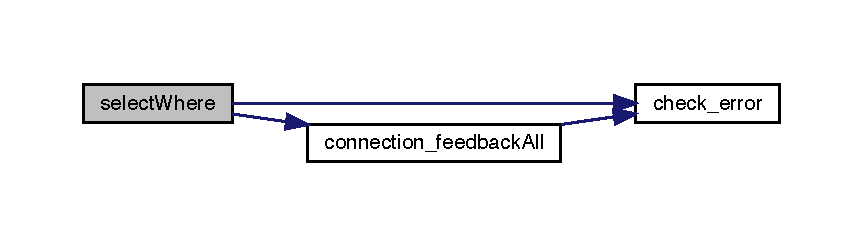
\includegraphics[width=350pt]{selection_request_8cpp_a90eb635de3f1856a45557b42f18eff28_cgraph}
\end{center}
\end{figure}
\mbox{\label{selection_request_8cpp_a519933061d4010c3a8d743b7e9fa9939}} 
\index{selection\+Request.\+cpp@{selection\+Request.\+cpp}!select\+Where\+One\+Column@{select\+Where\+One\+Column}}
\index{select\+Where\+One\+Column@{select\+Where\+One\+Column}!selection\+Request.\+cpp@{selection\+Request.\+cpp}}
\subsubsection{select\+Where\+One\+Column()}
{\footnotesize\ttfamily void select\+Where\+One\+Column (\begin{DoxyParamCaption}\item[{std\+::string}]{table\+Name,  }\item[{std\+::string}]{condition\+Column,  }\item[{std\+::string}]{condition\+Value }\end{DoxyParamCaption})}



Bestimmte Datensätze von bestimmten Spalten abfragen. 

Mithilfe der \char`\"{}select\+One\+Column\char`\"{} Methode werden S\+Q\+L-\/\+Abfragen nur bestimmter Datensätze in einer bestimmten Spalten abgefragt.~\newline
 Es wird nur die Spalte angzeigt, wo der Datensatz verglichen worden ist.~\newline


S\+Q\+L-\/\+Befehl\+: \char`\"{}\+S\+E\+L\+E\+C\+T $\ast$ F\+R\+O\+M \char`\"{} + table\+Name + \char`\"{} W\+H\+E\+R\+E \char`\"{} + condition\+Column + \char`\"{} = \char`\"{} + \char`\"{}\textquotesingle{}\char`\"{} + condition\+Value + \char`\"{}\textquotesingle{};\char`\"{} ~\newline



\begin{DoxyParams}{Parameter}
{\em table\+Name} & = Name der Tabelle \\
\hline
{\em condition\+Column} & = Enthält den Namen der Bedingungsspalte \\
\hline
{\em condition\+Value} & = Enthält den Bedingungswert\\
\hline
\end{DoxyParams}
\begin{DoxyReturn}{Rückgabe}
void  Die Funktion gibt ein void zurück -\/$>$ to Do sollte einen Boolean zurückgeben, ob der Befehl erfolgreich bearbeitet wurde.
\end{DoxyReturn}
\begin{DoxyAuthor}{Autor}
Martin Meyer 

Steffen Extra 
\end{DoxyAuthor}
Hier ist ein Graph, der zeigt, was diese Funktion aufruft\+:\nopagebreak
\begin{figure}[H]
\begin{center}
\leavevmode
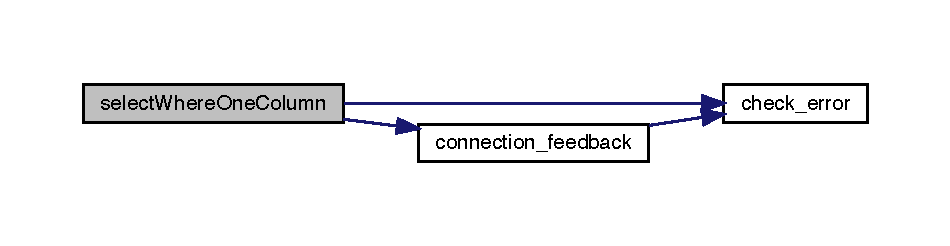
\includegraphics[width=350pt]{selection_request_8cpp_a519933061d4010c3a8d743b7e9fa9939_cgraph}
\end{center}
\end{figure}
\mbox{\label{selection_request_8cpp_a94269766ff6e39ba8a38f5623314c3cd}} 
\index{selection\+Request.\+cpp@{selection\+Request.\+cpp}!select\+Where\+Order\+By@{select\+Where\+Order\+By}}
\index{select\+Where\+Order\+By@{select\+Where\+Order\+By}!selection\+Request.\+cpp@{selection\+Request.\+cpp}}
\subsubsection{select\+Where\+Order\+By()}
{\footnotesize\ttfamily void select\+Where\+Order\+By (\begin{DoxyParamCaption}\item[{std\+::string}]{table\+Name,  }\item[{std\+::vector$<$ std\+::string $>$}]{columns,  }\item[{std\+::string}]{condition\+Column,  }\item[{std\+::string}]{condition\+Value,  }\item[{std\+::string}]{to\+Sortcolumn\+Name,  }\item[{std\+::string}]{sort\+By }\end{DoxyParamCaption})}



Abfrage von Spalten mit Sortierung. 

Mithilfe der \char`\"{}select\+Where\+Order\+By\char`\"{} Methode werden die S\+QL Abfragen nur bestimmter Datensätze in einer bestimmten Spalten abgefragt. Es werden die Spalten angezeigt, die der Nutzer in dem Vektor übergeben hat. Zudem wird es Aufsteigend oder Absteigend sortiert.

S\+Q\+L-\/\+Befehl für A\+SC\+: \char`\"{}\+S\+E\+L\+E\+C\+T \char`\"{} + all\+Columns + \char`\"{} F\+R\+O\+M \char`\"{} + table\+Name + \char`\"{} W\+H\+E\+R\+E \char`\"{} + condition\+Column + \char`\"{} = \textquotesingle{}\char`\"{} + condition\+Value + \char`\"{}\textquotesingle{}\char`\"{} + \char`\"{} O\+R\+D\+E\+R B\+Y \char`\"{} + to\+Sortcolumn\+Name + \char`\"{} A\+S\+C;\char`\"{} S\+Q\+L-\/\+Befehl für D\+E\+SC\+: \char`\"{}\+S\+E\+L\+E\+C\+T \char`\"{} + all\+Columns + \char`\"{} F\+R\+O\+M \char`\"{} + table\+Name + \char`\"{} W\+H\+E\+R\+E \char`\"{} + condition\+Column + \char`\"{} = \textquotesingle{}\char`\"{} + condition\+Value + \char`\"{}\textquotesingle{}\char`\"{} + \char`\"{} O\+R\+D\+E\+R B\+Y \char`\"{} + to\+Sortcolumn\+Name + \char`\"{} D\+E\+S\+C;\char`\"{}


\begin{DoxyParams}{Parameter}
{\em table\+Name} & = Name der Tabelle \\
\hline
{\em columns} & = Enthält die Liste der angezeigten Spalten \\
\hline
{\em condition\+Column} & = Enhält den Namen der Bedingungsspalte \\
\hline
{\em condition\+Value} & =Enhält den Bedingungswert \\
\hline
{\em to\+Sort\+Column\+Name} & =Enhält die Spalte zu der sotiert werden soll \\
\hline
{\em Sort\+By} & = Gibt an ob es Aufsteigend bzw Absteigend sotoiert werden soll\\
\hline
\end{DoxyParams}
\begin{DoxyReturn}{Rückgabe}
void
\end{DoxyReturn}
\begin{DoxyAuthor}{Autor}
Martin Meyer 

Steffen Extra 
\end{DoxyAuthor}
Hier ist ein Graph, der zeigt, was diese Funktion aufruft\+:\nopagebreak
\begin{figure}[H]
\begin{center}
\leavevmode
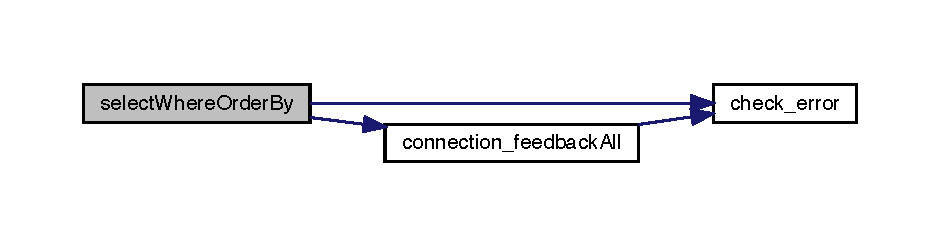
\includegraphics[width=350pt]{selection_request_8cpp_a94269766ff6e39ba8a38f5623314c3cd_cgraph}
\end{center}
\end{figure}
\mbox{\label{selection_request_8cpp_a1bde570da9c90a3d0f6e94bc1b06c5e3}} 
\index{selection\+Request.\+cpp@{selection\+Request.\+cpp}!union\+Select@{union\+Select}}
\index{union\+Select@{union\+Select}!selection\+Request.\+cpp@{selection\+Request.\+cpp}}
\subsubsection{union\+Select()}
{\footnotesize\ttfamily void union\+Select (\begin{DoxyParamCaption}\item[{std\+::vector$<$ std\+::string $>$}]{table\+Name,  }\item[{std\+::vector$<$ std\+::string $>$}]{column\+Name }\end{DoxyParamCaption})}



Vereinigung zweier Abfragen. 

Die \char`\"{}union\+Select\char`\"{} Methode vereinigt die Ergebnisse zweier Abfragen.~\newline


S\+Q\+L-\/\+Befehl\+: \char`\"{}\+S\+E\+L\+E\+C\+T \char`\"{} + column\+Name.\+at(i) + \char`\"{} F\+R\+O\+M \char`\"{} + table\+Name.\+at(i) + \char`\"{} U\+N\+I\+O\+N \char`\"{};


\begin{DoxyParams}{Parameter}
{\em table\+Name} & = Enthält die Liste der Tabellennamen \\
\hline
{\em column\+Name} & = Enthält die Liste der Spaltennamen\\
\hline
\end{DoxyParams}
\begin{DoxyReturn}{Rückgabe}
void
\end{DoxyReturn}
\begin{DoxyAuthor}{Autor}
Martin Meyer 

Steffen Extra 
\end{DoxyAuthor}
Hier ist ein Graph, der zeigt, was diese Funktion aufruft\+:\nopagebreak
\begin{figure}[H]
\begin{center}
\leavevmode
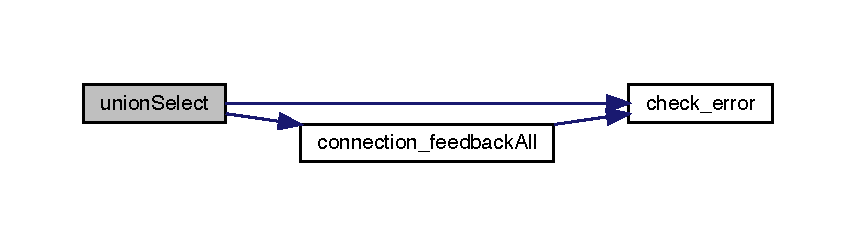
\includegraphics[width=350pt]{selection_request_8cpp_a1bde570da9c90a3d0f6e94bc1b06c5e3_cgraph}
\end{center}
\end{figure}

\section{sqllib.\+hpp-\/\+Dateireferenz}
\label{sqllib_8hpp}\index{sqllib.\+hpp@{sqllib.\+hpp}}
{\ttfamily \#include $<$string$>$}\newline
{\ttfamily \#include $<$iostream$>$}\newline
{\ttfamily \#include $<$stdio.\+h$>$}\newline
{\ttfamily \#include $<$stdlib.\+h$>$}\newline
{\ttfamily \#include $<$unistd.\+h$>$}\newline
{\ttfamily \#include $<$vector$>$}\newline
Include-\/\+Abhängigkeitsdiagramm für sqllib.\+hpp\+:\nopagebreak
\begin{figure}[H]
\begin{center}
\leavevmode
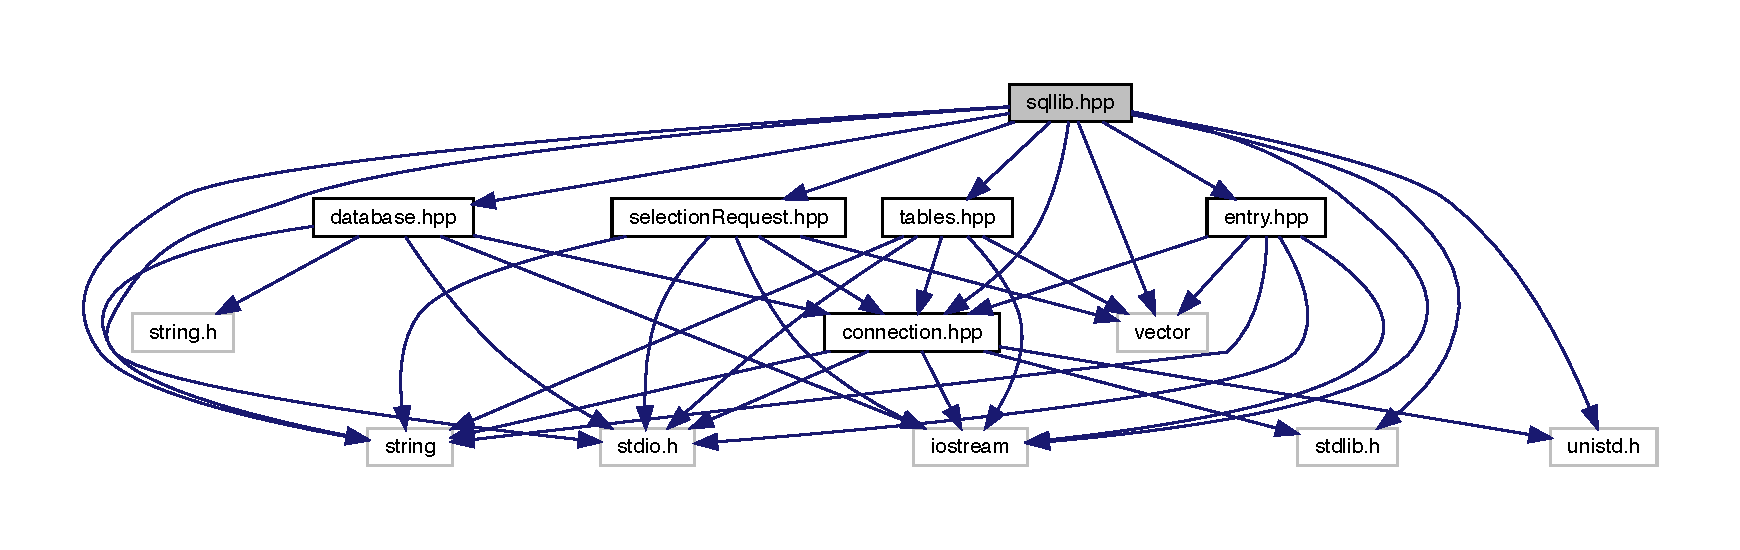
\includegraphics[width=350pt]{sqllib_8hpp__incl}
\end{center}
\end{figure}
Dieser Graph zeigt, welche Datei direkt oder indirekt diese Datei enthält\+:\nopagebreak
\begin{figure}[H]
\begin{center}
\leavevmode
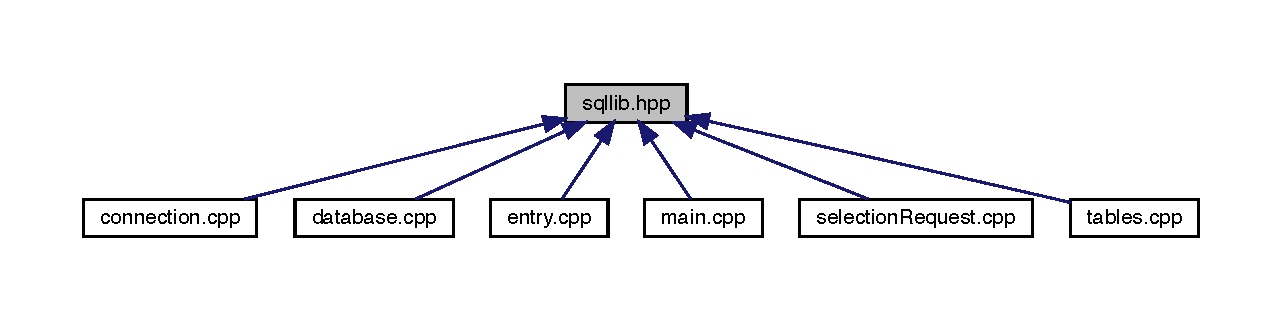
\includegraphics[width=350pt]{sqllib_8hpp__dep__incl}
\end{center}
\end{figure}
\subsection*{Funktionen}
\begin{DoxyCompactItemize}
\item 
void \textbf{ check\+\_\+error} (void)
\begin{DoxyCompactList}\small\item\em Fehlermethode. \end{DoxyCompactList}\item 
void \textbf{ connection\+\_\+feedback} (std\+::string sql\+Command)
\begin{DoxyCompactList}\small\item\em Rückgabe einzelner Ergebnisse. \end{DoxyCompactList}\item 
void \textbf{ connection\+\_\+feedback\+All} (std\+::string sql\+Command)
\begin{DoxyCompactList}\small\item\em Rückgabe aller Datensätze. \end{DoxyCompactList}\item 
void \textbf{ connection\+\_\+query} (std\+::string sqlcommand)
\begin{DoxyCompactList}\small\item\em Sendet eine Abfrage zum S\+Q\+L-\/\+Server. \end{DoxyCompactList}\item 
void \textbf{ connectionless} (const char $\ast$host, const char $\ast$user, const char $\ast$passwort, const char $\ast$db, unsigned int port, const char $\ast$unix\+\_\+socket, unsigned int client\+\_\+flag)
\item 
void \textbf{ disconnect} ()
\begin{DoxyCompactList}\small\item\em Verbindung schließen. \end{DoxyCompactList}\item 
void \textbf{ create\+Database} (std\+::string database\+Name)
\begin{DoxyCompactList}\small\item\em Erstellen einer Datenbank. \end{DoxyCompactList}\item 
void \textbf{ show\+Databases} ()
\begin{DoxyCompactList}\small\item\em Anzeigen der Datenbanken. \end{DoxyCompactList}\item 
void \textbf{ rename\+Database} (std\+::string database\+Name, std\+::string new\+Database\+Name)
\begin{DoxyCompactList}\small\item\em Datenbanknamen ändern. \end{DoxyCompactList}\item 
void \textbf{ delete\+Database} (std\+::string database\+Name)
\begin{DoxyCompactList}\small\item\em Löschen einer Datenbank. \end{DoxyCompactList}\item 
void \textbf{ create\+Table} (bool primary\+\_\+key, std\+::string table\+Name, std\+::vector$<$ std\+::string $>$ columns)
\item 
void \textbf{ show\+Table} (std\+::string table\+Name)
\begin{DoxyCompactList}\small\item\em Ausgabe der Tabelle. \end{DoxyCompactList}\item 
void \textbf{ rename\+Table} (std\+::string tablename, std\+::string new\+Table\+Name)
\begin{DoxyCompactList}\small\item\em Änderung des Tabellennamens. \end{DoxyCompactList}\item 
void \textbf{ delete\+Table} (std\+::string table\+Name)
\begin{DoxyCompactList}\small\item\em Löschen einer Tabelle. \end{DoxyCompactList}\item 
void \textbf{ set\+Column} (std\+::string table\+Name, std\+::string Column\+Name, std\+::string datatype)
\begin{DoxyCompactList}\small\item\em Bearbeiten der Spalte in einer Tabelle. \end{DoxyCompactList}\item 
void \textbf{ set\+Column\+With\+Primary} (std\+::string table\+Name, std\+::string Column\+Name, std\+::string datatype, bool autoinc)
\begin{DoxyCompactList}\small\item\em Setzen des Primärschlüssels. \end{DoxyCompactList}\item 
void \textbf{ modifier\+Column\+Name} (std\+::string table\+Name, std\+::string old\+Column\+Name, std\+::string new\+Column\+Name, std\+::string datatype)
\begin{DoxyCompactList}\small\item\em Modifizieren des Spaltennamens. \end{DoxyCompactList}\item 
void \textbf{ change\+The\+Datatype} (std\+::string table\+Name, std\+::string column\+Name, std\+::string datatype)
\begin{DoxyCompactList}\small\item\em Ändern des Datentyps. \end{DoxyCompactList}\item 
void \textbf{ get\+All\+Column} (std\+::string table\+Name)
\begin{DoxyCompactList}\small\item\em Anzeigen von Spalten. \end{DoxyCompactList}\item 
void \textbf{ count\+Datasets} (std\+::string table\+Name)
\begin{DoxyCompactList}\small\item\em Zählen der Datensätze. \end{DoxyCompactList}\item 
void \textbf{ show\+Column\+Typ} (std\+::string table\+Name, std\+::string datatype)
\begin{DoxyCompactList}\small\item\em Datentyp der Spalte anzeigen lassen. \end{DoxyCompactList}\item 
void \textbf{ delete\+Column} (std\+::string table\+Name, std\+::string column\+Name)
\begin{DoxyCompactList}\small\item\em Löschen von Spalten. \end{DoxyCompactList}\item 
void \textbf{ set\+Secondary\+Key} (std\+::string table\+Name\+Secondary, std\+::string foreign\+Key, std\+::string table\+Name\+Primary, std\+::string primary\+Key, std\+::string constraint)
\begin{DoxyCompactList}\small\item\em Setzen des Sekundärschlüssels (Foreign Key) \end{DoxyCompactList}\item 
void \textbf{ delete\+Secondary\+Key} (std\+::string table\+Name, std\+::string constraint)
\begin{DoxyCompactList}\small\item\em Löschen des Sekundärschlüssels. \end{DoxyCompactList}\item 
void \textbf{ set\+Primary\+Key} (std\+::string table\+Name, std\+::string primary\+Key)
\begin{DoxyCompactList}\small\item\em Nachträgliches setzen eines Primärschlüssels. \end{DoxyCompactList}\item 
void \textbf{ delete\+Primary\+Key} (std\+::string table\+Name)
\begin{DoxyCompactList}\small\item\em Löschen des Primärschlüssels. \end{DoxyCompactList}\item 
void \textbf{ set\+Entry} (std\+::string table\+Name, std\+::string column\+Name, std\+::string entry)
\begin{DoxyCompactList}\small\item\em Erstellen eines Eintrags. \end{DoxyCompactList}\item 
void \textbf{ modifier\+Entry} (std\+::string table\+Name, std\+::string column\+Name, std\+::string old\+Entry, std\+::string new\+Entry)
\begin{DoxyCompactList}\small\item\em Einträge modifizieren. \end{DoxyCompactList}\item 
void \textbf{ set\+All\+Entry} (std\+::string table\+Name, std\+::vector$<$ std\+::string $>$ \textbf{ row})
\begin{DoxyCompactList}\small\item\em Beliebige Anzahl von Einträgen hinzufügen. \end{DoxyCompactList}\item 
void \textbf{ delete\+Entry} (std\+::string table\+Name, std\+::string column\+Name, std\+::string condition)
\begin{DoxyCompactList}\small\item\em Löschen von Einträgen. \end{DoxyCompactList}\item 
void \textbf{ own\+Command} (std\+::string sql\+Command, std\+::string command\+Type)
\begin{DoxyCompactList}\small\item\em Benutzereigener S\+Q\+L-\/\+Befehl. \end{DoxyCompactList}\item 
void \textbf{ select\+Like} (std\+::string table\+Name, std\+::vector$<$ std\+::string $>$columns, std\+::string to\+Search\+Column, std\+::string pattern, std\+::string to\+Search)
\begin{DoxyCompactList}\small\item\em Suche nach Muster. \end{DoxyCompactList}\item 
void \textbf{ select\+Not\+Like} (std\+::string table\+Name, std\+::vector$<$ std\+::string $>$columns, std\+::string to\+Search\+Column, std\+::string pattern, std\+::string to\+Search)
\begin{DoxyCompactList}\small\item\em Suche nach Muster. \end{DoxyCompactList}\item 
void \textbf{ select\+Min\+Or\+Max} (std\+::string table\+Name, std\+::string min\+Or\+Max, std\+::string min\+Or\+Max\+Column, std\+::string alias\+Column)
\begin{DoxyCompactList}\small\item\em Ermittlung des höchsten / niedrigsten Wertes. \end{DoxyCompactList}\item 
void \textbf{ select\+Min\+Or\+Max\+Where} (std\+::string table\+Name, std\+::string min\+Or\+Max, std\+::string min\+Or\+Max\+Column, std\+::string alias\+Column, std\+::string condition\+Column, std\+::string condition\+Value)
\begin{DoxyCompactList}\small\item\em Höchster / niedrigster Wert mit Bedingung und Alias-\/\+Spalte. \end{DoxyCompactList}\item 
void \textbf{ select\+Limit\+Where\+Order\+By} (std\+::string table\+Name, std\+::vector$<$ std\+::string $>$ columns, std\+::string limit\+Number, std\+::string condition\+Column, std\+::string condition\+Value, std\+::string to\+Sort\+Column\+Name, std\+::string sort\+By)
\begin{DoxyCompactList}\small\item\em Bestimmte Anzahl von Datensätzen mit Bedingung abfragen. \end{DoxyCompactList}\item 
void \textbf{ select\+Where\+One\+Column} (std\+::string table\+Name, std\+::string condition\+Column, std\+::string condition\+Value)
\begin{DoxyCompactList}\small\item\em Bestimmte Datensätze von bestimmten Spalten abfragen. \end{DoxyCompactList}\item 
void \textbf{ select\+Where} (std\+::string table\+Name, std\+::vector$<$ std\+::string $>$ columns, std\+::string condition\+Column, std\+::string condition\+Value)
\begin{DoxyCompactList}\small\item\em Anzeigen bestimmter Datensätze mit dem Zusatz der Where-\/\+Clause. \end{DoxyCompactList}\item 
void \textbf{ select\+Where\+Bool} (std\+::string table\+Name, std\+::vector$<$ std\+::string $>$ columns, std\+::vector$<$ std\+::string $>$conditions, std\+::vector$<$ std\+::string $>$condition\+Value, std\+::vector$<$ std\+::string $>$ conditions2, std\+::vector$<$ std\+::string $>$condition\+Value2, std\+::vector$<$ std\+::string $>$operators)
\item 
void \textbf{ select\+Where\+Order\+By} (std\+::string table\+Name, std\+::vector$<$ std\+::string $>$ columns, std\+::string condition\+Column, std\+::string condition\+Value, std\+::string to\+Sortcolumn\+Name, std\+::string sort\+By)
\begin{DoxyCompactList}\small\item\em Abfrage von Spalten mit Sortierung. \end{DoxyCompactList}\item 
void \textbf{ select\+Sort\+Table} (std\+::string table\+Name, std\+::string to\+Sort\+Column\+Name, std\+::string sort\+By)
\begin{DoxyCompactList}\small\item\em Tabelle wird nach Angabe sortiert. \end{DoxyCompactList}\item 
void \textbf{ select\+Count} (std\+::string table\+Name, std\+::string count\+Column, std\+::string alias\+Column\+Name)
\begin{DoxyCompactList}\small\item\em Anzahl von ausgewählten Datensätzen. \end{DoxyCompactList}\item 
void \textbf{ select\+Distinct} (std\+::string table\+Name, std\+::vector$<$ std\+::string $>$ columns)
\begin{DoxyCompactList}\small\item\em Redundanzen werden eliminiert und nur einmal angezeigt. \end{DoxyCompactList}\item 
void \textbf{ select\+Count\+Distinct} (std\+::string table\+Name, std\+::string count\+Column)
\begin{DoxyCompactList}\small\item\em Keine Redundanzen / Datensätze werden gezählt. \end{DoxyCompactList}\item 
void \textbf{ select\+Average\+Sum} (std\+::string table\+Name, std\+::string column\+Name)
\begin{DoxyCompactList}\small\item\em Durchschnittswert. \end{DoxyCompactList}\item 
void \textbf{ select\+Sum} (std\+::string table\+Name, std\+::string column\+Name, std\+::string alias\+Column\+Name)
\begin{DoxyCompactList}\small\item\em Summieren von Werten. \end{DoxyCompactList}\item 
void \textbf{ union\+Select} (std\+::vector$<$ std\+::string $>$ table\+Name, std\+::vector$<$ std\+::string $>$ column\+Name)
\begin{DoxyCompactList}\small\item\em Vereinigung zweier Abfragen. \end{DoxyCompactList}\item 
void \textbf{ select\+In} (std\+::string table\+Name, std\+::vector$<$ std\+::string $>$columns, std\+::string search\+In\+Column, std\+::vector$<$ std\+::string $>$condition\+Value)
\begin{DoxyCompactList}\small\item\em Mehrere Abfrageergebnisse bündeln. \end{DoxyCompactList}\item 
void \textbf{ select\+Between} (std\+::string condition\+String, std\+::string condition\+String\+Two, std\+::string table\+Name, std\+::string condition\+Column, std\+::string condition\+Column\+Two, std\+::string condition, std\+::string condition\+Two)
\begin{DoxyCompactList}\small\item\em Eingeschränkte Abfragen. \end{DoxyCompactList}\item 
void \textbf{ select\+Columns\+Alias} (std\+::string table\+Name, std\+::vector$<$ std\+::string $>$columns, std\+::vector$<$ std\+::string $>$aliases)
\begin{DoxyCompactList}\small\item\em Alias-\/\+Spaltennamen. \end{DoxyCompactList}\item 
void \textbf{ select\+Table\+Alias} (std\+::string table\+Name, std\+::vector$<$ std\+::string $>$columns, std\+::string alias\+Table\+Name)
\begin{DoxyCompactList}\small\item\em Zuweisung eines Alias. \end{DoxyCompactList}\item 
void \textbf{ select\+Group\+By} (std\+::string table\+Name, std\+::vector$<$ std\+::string $>$columns, std\+::string condition\+Column, std\+::string condition\+Value, std\+::vector$<$ std\+::string $>$group\+By\+Columns)
\begin{DoxyCompactList}\small\item\em Gruppieren von Ergebnismengen. \end{DoxyCompactList}\item 
void \textbf{ select\+Group\+By\+Order\+By} (std\+::string table\+Name, std\+::vector$<$ std\+::string $>$columns, std\+::string condition\+Column, std\+::string condition\+Value, std\+::vector$<$ std\+::string $>$group\+By\+Columns, std\+::string to\+Sortcolumn\+Name, std\+::string sort\+By)
\begin{DoxyCompactList}\small\item\em Ergebnismengen + sortieren. \end{DoxyCompactList}\item 
void \textbf{ select\+Count\+Group\+By\+Order\+By} (std\+::string table\+Name, std\+::string count\+Column, std\+::vector$<$ std\+::string $>$columns, std\+::string condition\+Column, std\+::string condition\+Value, std\+::vector$<$ std\+::string $>$group\+By\+Columns, std\+::string sort\+By)
\begin{DoxyCompactList}\small\item\em Ergebnismengen gruppieren + zählen der Datensätze + Sortierung. \end{DoxyCompactList}\item 
void \textbf{ select\+Null} (std\+::string table\+Name, std\+::string column\+Name)
\begin{DoxyCompactList}\small\item\em N\+U\+LL Werte. \end{DoxyCompactList}\item 
void \textbf{ select\+Inner\+Join} (std\+::string first\+Table\+Name, std\+::string column\+I\+D\+Table\+One, std\+::vector$<$ std\+::string $>$ columns\+Table\+One, std\+::string second\+Table\+Name, std\+::vector$<$ std\+::string $>$ columns\+Table\+Two)
\begin{DoxyCompactList}\small\item\em Inner\+Join-\/\+Befehl. \end{DoxyCompactList}\item 
void \textbf{ select\+Left\+Join} (std\+::string first\+Table\+Name, std\+::string column\+I\+D\+Table\+One, std\+::vector$<$ std\+::string $>$ columns\+Table\+One, std\+::string second\+Table\+Name, std\+::vector$<$ std\+::string $>$ columns\+Table\+Two)
\begin{DoxyCompactList}\small\item\em Left\+Join Methode. \end{DoxyCompactList}\item 
void \textbf{ select\+Right\+Join} (std\+::string first\+Table\+Name, std\+::string column\+I\+D\+Table\+One, std\+::vector$<$ std\+::string $>$ columns\+Table\+One, std\+::string second\+Table\+Name, std\+::vector$<$ std\+::string $>$ columns\+Table\+Two)
\item 
void \textbf{ select\+Full\+Join} (std\+::string first\+Table\+Name, std\+::string column\+I\+D\+Table\+One, std\+::vector$<$ std\+::string $>$ columns\+Table\+One, std\+::string second\+Table\+Name, std\+::vector$<$ std\+::string $>$ columns\+Table\+Two)
\begin{DoxyCompactList}\small\item\em Full\+Join Methode. \end{DoxyCompactList}\end{DoxyCompactItemize}


\subsection{Dokumentation der Funktionen}
\mbox{\label{sqllib_8hpp_aef4d6b8ba9c38e5f1b459694421ad9e5}} 
\index{sqllib.\+hpp@{sqllib.\+hpp}!change\+The\+Datatype@{change\+The\+Datatype}}
\index{change\+The\+Datatype@{change\+The\+Datatype}!sqllib.\+hpp@{sqllib.\+hpp}}
\subsubsection{change\+The\+Datatype()}
{\footnotesize\ttfamily void change\+The\+Datatype (\begin{DoxyParamCaption}\item[{std\+::string}]{table\+Name,  }\item[{std\+::string}]{column\+Name,  }\item[{std\+::string}]{datatype }\end{DoxyParamCaption})}



Ändern des Datentyps. 

Ändern des Datentyps einer Spalte ohne den Namen der Spalte zu ändern. ~\newline
 Wenn der Datentyp der Spalte geändert wird, muss darauf geachtet werden, dass die Objekte in der Spalte dem Datentyp entsprechen. ~\newline


S\+Q\+L-\/\+Befehl\+: \char`\"{}\+Al\+T\+E\+R T\+A\+B\+L\+E \char`\"{} + table\+Name + \char`\"{} M\+O\+D\+I\+F\+Y \char`\"{} + column\+Name + \char`\"{} \char`\"{} + datatype;


\begin{DoxyParams}{Parameter}
{\em table\+Name} & = Name der Tabelle \\
\hline
{\em column\+Name} & = Name der Spalte \\
\hline
{\em datatype} & = Neuer Datentyp\\
\hline
\end{DoxyParams}
\begin{DoxyReturn}{Rückgabe}
void
\end{DoxyReturn}
\begin{DoxyAuthor}{Autor}
Steffen Extra 
\end{DoxyAuthor}
Hier ist ein Graph, der zeigt, was diese Funktion aufruft\+:\nopagebreak
\begin{figure}[H]
\begin{center}
\leavevmode
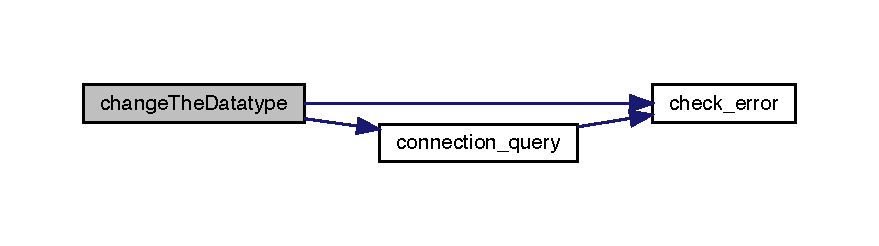
\includegraphics[width=350pt]{sqllib_8hpp_aef4d6b8ba9c38e5f1b459694421ad9e5_cgraph}
\end{center}
\end{figure}
\mbox{\label{sqllib_8hpp_a33fd832a9e1a27bddb7d9837a2dcf2f1}} 
\index{sqllib.\+hpp@{sqllib.\+hpp}!check\+\_\+error@{check\+\_\+error}}
\index{check\+\_\+error@{check\+\_\+error}!sqllib.\+hpp@{sqllib.\+hpp}}
\subsubsection{check\+\_\+error()}
{\footnotesize\ttfamily void check\+\_\+error (\begin{DoxyParamCaption}\item[{void}]{ }\end{DoxyParamCaption})}



Fehlermethode. 

yolo \subsection{Introduction}\label{sqllib_8hpp_intro}
This is the introduction.\subsection{Installation}\label{sqllib_8hpp_install}
\subsubsection{Step 1\+: Opening the box}\label{sqllib_8hpp_step1}
etc... ~\newline
 /def Je nach Betriebssystem wird der Pfad für die mysql-\/\+Headerdatei includiert

Die Methode \char`\"{}check\+\_\+error\char`\"{} ist verantwortlich für die Ausnahme, die ausgelöst wird, wenn My\+S\+QL einen Fehler zurückgibt.~\newline



\begin{DoxyParams}{Parameter}
{\em -\/} & \\
\hline
\end{DoxyParams}
\begin{DoxyReturn}{Rückgabe}
void
\end{DoxyReturn}
\begin{DoxyAuthor}{Autor}
Martin Meyer 

Steffen Extra 
\end{DoxyAuthor}
\mbox{\label{sqllib_8hpp_ab12a404eefae07281e8d1273ca3fc447}} 
\index{sqllib.\+hpp@{sqllib.\+hpp}!connection\+\_\+feedback@{connection\+\_\+feedback}}
\index{connection\+\_\+feedback@{connection\+\_\+feedback}!sqllib.\+hpp@{sqllib.\+hpp}}
\subsubsection{connection\+\_\+feedback()}
{\footnotesize\ttfamily void connection\+\_\+feedback (\begin{DoxyParamCaption}\item[{std\+::string}]{sql\+Command }\end{DoxyParamCaption})}



Rückgabe einzelner Ergebnisse. 

Die Methode \char`\"{}connection\+\_\+feedback\char`\"{} liefert eine Spalte des aktuellen Datensatzes.~\newline
 Diese wird benutzt um einzelne Ergebnis zurückzugeben. (Bspw. \doxyref{select\+Count()}{S.}{selection_request_8cpp_a00f071477f164f70927ee9923dd77a39} )


\begin{DoxyParams}{Parameter}
{\em sql\+Command} & = enthält den auszuführenden S\+Q\+L-\/\+Befehl\\
\hline
\end{DoxyParams}
\begin{DoxyReturn}{Rückgabe}
void
\end{DoxyReturn}
\begin{DoxyAuthor}{Autor}
Martin Meyer 

Steffen Extra 
\end{DoxyAuthor}
Hier ist ein Graph, der zeigt, was diese Funktion aufruft\+:\nopagebreak
\begin{figure}[H]
\begin{center}
\leavevmode
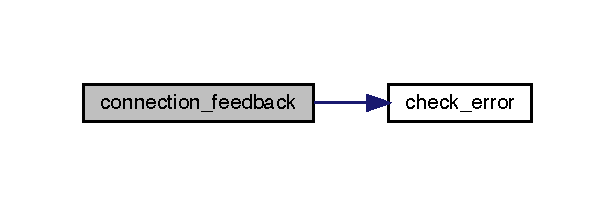
\includegraphics[width=295pt]{sqllib_8hpp_ab12a404eefae07281e8d1273ca3fc447_cgraph}
\end{center}
\end{figure}
Hier ist ein Graph der zeigt, wo diese Funktion aufgerufen wird\+:\nopagebreak
\begin{figure}[H]
\begin{center}
\leavevmode
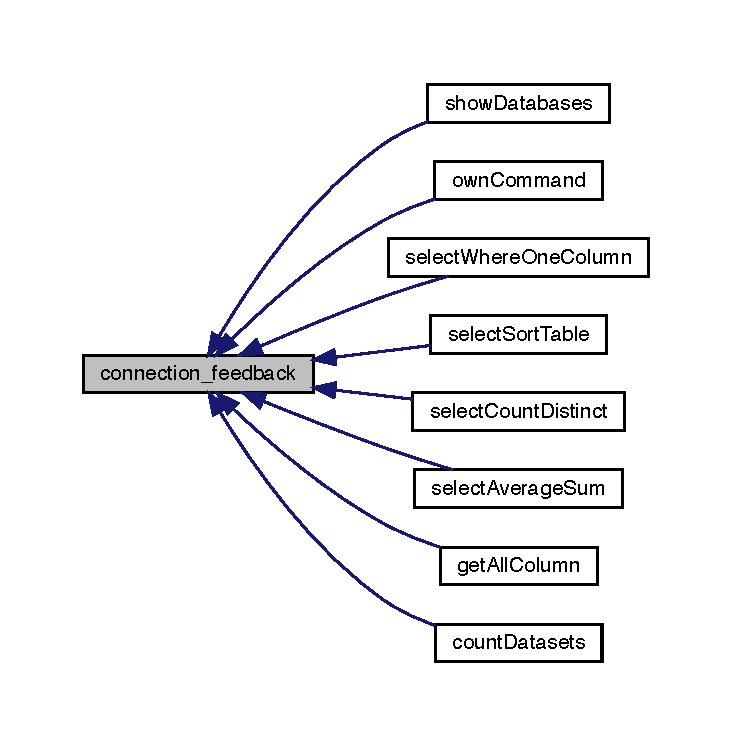
\includegraphics[width=350pt]{sqllib_8hpp_ab12a404eefae07281e8d1273ca3fc447_icgraph}
\end{center}
\end{figure}
\mbox{\label{sqllib_8hpp_a05a069b8d1bef185dd0ff85424e2e13c}} 
\index{sqllib.\+hpp@{sqllib.\+hpp}!connection\+\_\+feedback\+All@{connection\+\_\+feedback\+All}}
\index{connection\+\_\+feedback\+All@{connection\+\_\+feedback\+All}!sqllib.\+hpp@{sqllib.\+hpp}}
\subsubsection{connection\+\_\+feedback\+All()}
{\footnotesize\ttfamily void connection\+\_\+feedback\+All (\begin{DoxyParamCaption}\item[{std\+::string}]{sql\+Command }\end{DoxyParamCaption})}



Rückgabe aller Datensätze. 

Die Methode \char`\"{}connection\+\_\+feedback\+All\char`\"{} liefert den kompletten Datensatz zurück der Abfrage zurück.


\begin{DoxyParams}{Parameter}
{\em sql\+Command} & = enhält den auszuführenden S\+Q\+L-\/\+Befehl\\
\hline
\end{DoxyParams}
\begin{DoxyReturn}{Rückgabe}
void
\end{DoxyReturn}
\begin{DoxyAuthor}{Autor}
Martin Meyer 

Steffen Extra 
\end{DoxyAuthor}
Hier ist ein Graph, der zeigt, was diese Funktion aufruft\+:\nopagebreak
\begin{figure}[H]
\begin{center}
\leavevmode
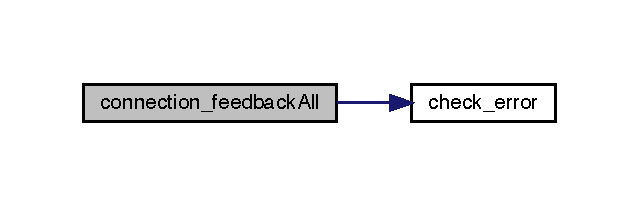
\includegraphics[width=306pt]{sqllib_8hpp_a05a069b8d1bef185dd0ff85424e2e13c_cgraph}
\end{center}
\end{figure}
Hier ist ein Graph der zeigt, wo diese Funktion aufgerufen wird\+:\nopagebreak
\begin{figure}[H]
\begin{center}
\leavevmode
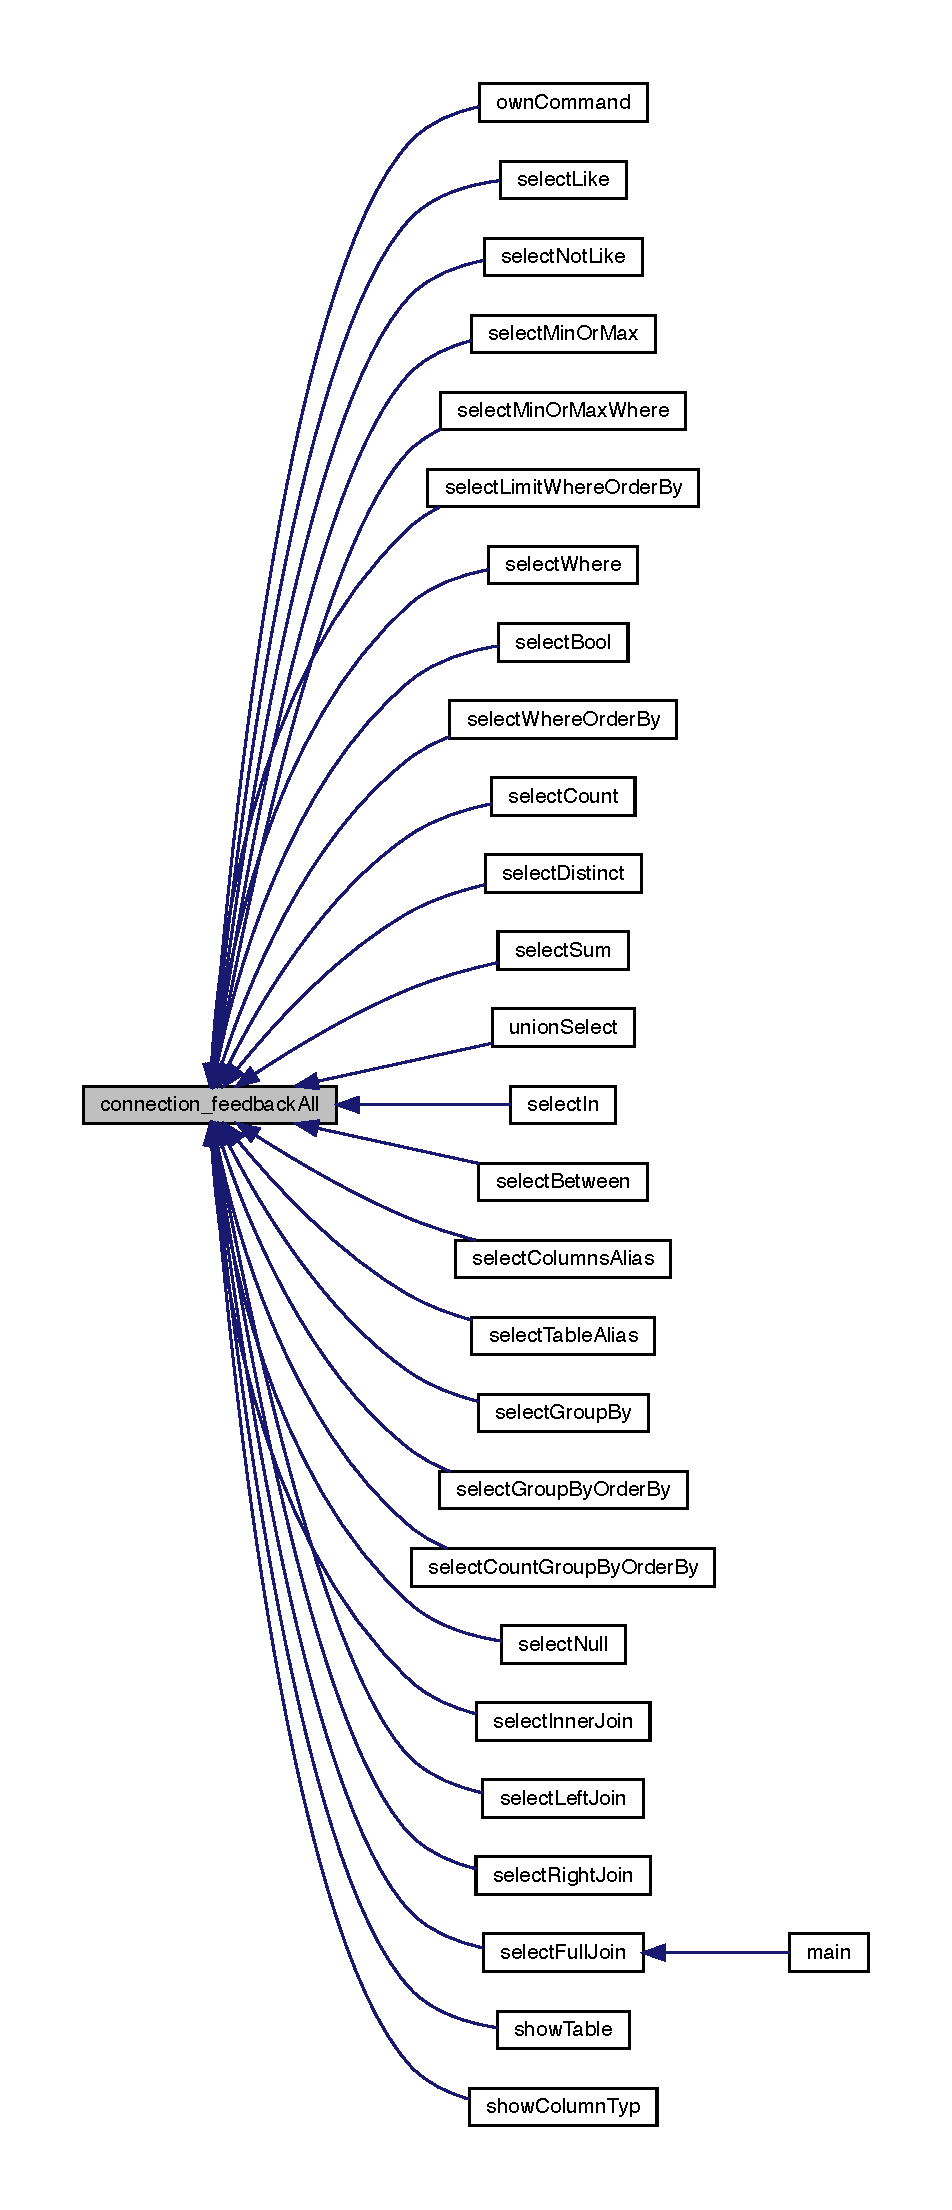
\includegraphics[height=550pt]{sqllib_8hpp_a05a069b8d1bef185dd0ff85424e2e13c_icgraph}
\end{center}
\end{figure}
\mbox{\label{sqllib_8hpp_a83d389dd4406da88cf16f7736e012537}} 
\index{sqllib.\+hpp@{sqllib.\+hpp}!connection\+\_\+query@{connection\+\_\+query}}
\index{connection\+\_\+query@{connection\+\_\+query}!sqllib.\+hpp@{sqllib.\+hpp}}
\subsubsection{connection\+\_\+query()}
{\footnotesize\ttfamily void connection\+\_\+query (\begin{DoxyParamCaption}\item[{std\+::string}]{sql\+Command }\end{DoxyParamCaption})}



Sendet eine Abfrage zum S\+Q\+L-\/\+Server. 

Die Methode \char`\"{}connection\+\_\+query\char`\"{} sendet eine eindeutige Abfrage (mehrere Abfragen werden nicht unterstützt) an die derzeit aktive Datenbank auf dem Server, der dem angegebenen Server zugeordnet ist. ~\newline



\begin{DoxyParams}{Parameter}
{\em sql\+Command} & = enhält den auszuführenden S\+Q\+L-\/\+Befehl\\
\hline
\end{DoxyParams}
\begin{DoxyReturn}{Rückgabe}
void
\end{DoxyReturn}
\begin{DoxyAuthor}{Autor}
Martin Meyer 

Steffen Extra 
\end{DoxyAuthor}
Hier ist ein Graph, der zeigt, was diese Funktion aufruft\+:\nopagebreak
\begin{figure}[H]
\begin{center}
\leavevmode
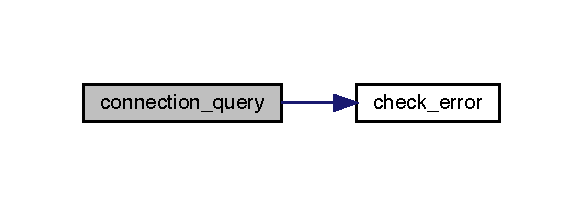
\includegraphics[width=280pt]{sqllib_8hpp_a83d389dd4406da88cf16f7736e012537_cgraph}
\end{center}
\end{figure}
Hier ist ein Graph der zeigt, wo diese Funktion aufgerufen wird\+:\nopagebreak
\begin{figure}[H]
\begin{center}
\leavevmode
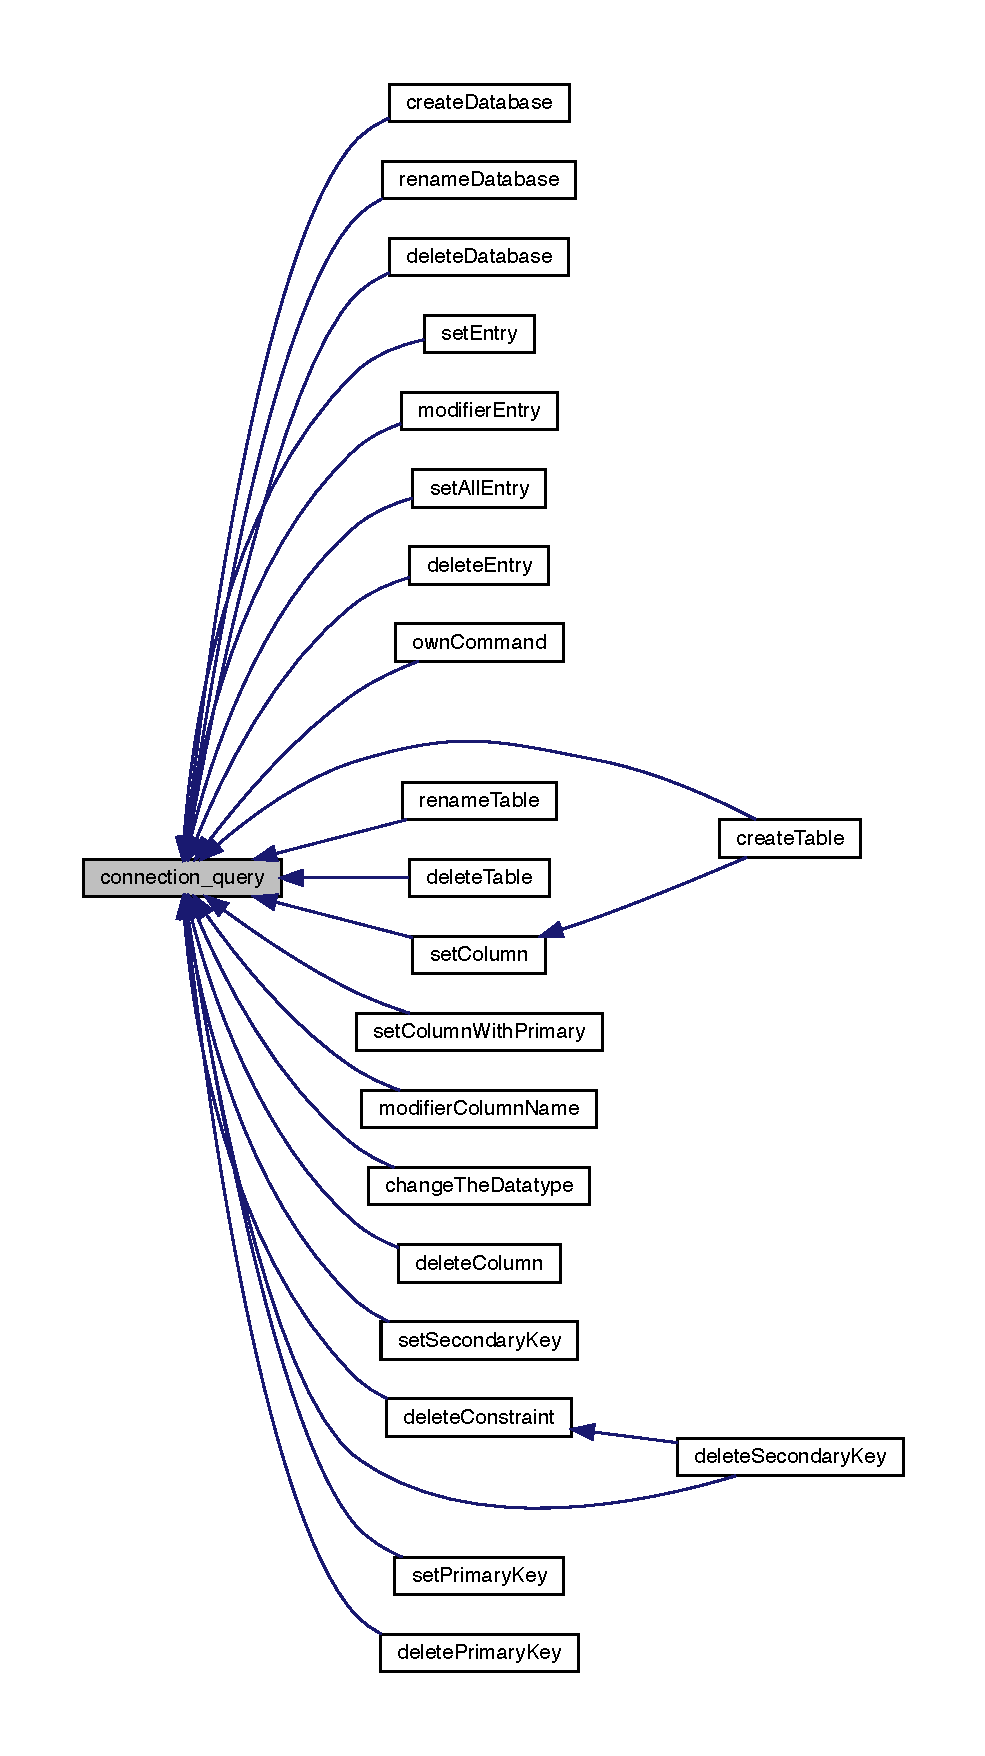
\includegraphics[height=550pt]{sqllib_8hpp_a83d389dd4406da88cf16f7736e012537_icgraph}
\end{center}
\end{figure}
\mbox{\label{sqllib_8hpp_a76ac4f4e873cad05bcaa10a8b7e048ce}} 
\index{sqllib.\+hpp@{sqllib.\+hpp}!connectionless@{connectionless}}
\index{connectionless@{connectionless}!sqllib.\+hpp@{sqllib.\+hpp}}
\subsubsection{connectionless()}
{\footnotesize\ttfamily void connectionless (\begin{DoxyParamCaption}\item[{const char $\ast$}]{host,  }\item[{const char $\ast$}]{user,  }\item[{const char $\ast$}]{passwort,  }\item[{const char $\ast$}]{db,  }\item[{unsigned int}]{port,  }\item[{const char $\ast$}]{unix\+\_\+socket,  }\item[{unsigned int}]{client\+\_\+flag }\end{DoxyParamCaption})}

\mbox{\label{sqllib_8hpp_ad2178bf4577d7eea6caebd8d1c942088}} 
\index{sqllib.\+hpp@{sqllib.\+hpp}!count\+Datasets@{count\+Datasets}}
\index{count\+Datasets@{count\+Datasets}!sqllib.\+hpp@{sqllib.\+hpp}}
\subsubsection{count\+Datasets()}
{\footnotesize\ttfamily void count\+Datasets (\begin{DoxyParamCaption}\item[{std\+::string}]{table\+Name }\end{DoxyParamCaption})}



Zählen der Datensätze. 

Alle Datensätze werden gezählt und ausgegeben.~\newline


S\+Q\+L-\/\+Befehl\+: \char`\"{}\+S\+E\+L\+E\+C\+T C\+O\+U\+N\+T ($\ast$) F\+R\+O\+M \char`\"{} + table\+Name;


\begin{DoxyParams}{Parameter}
{\em table\+Name} & = Name der Tabelle;\\
\hline
\end{DoxyParams}
\begin{DoxyReturn}{Rückgabe}
void
\end{DoxyReturn}
\begin{DoxyAuthor}{Autor}
Steffen Extra 
\end{DoxyAuthor}
Hier ist ein Graph, der zeigt, was diese Funktion aufruft\+:\nopagebreak
\begin{figure}[H]
\begin{center}
\leavevmode
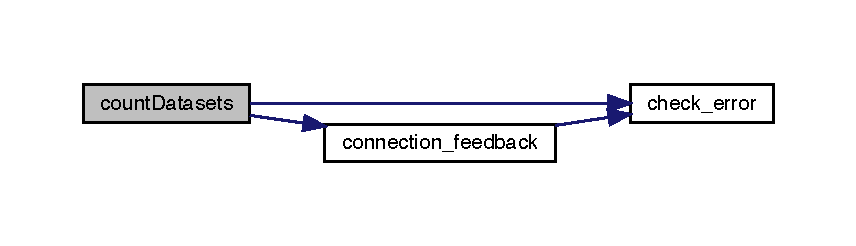
\includegraphics[width=350pt]{sqllib_8hpp_ad2178bf4577d7eea6caebd8d1c942088_cgraph}
\end{center}
\end{figure}
\mbox{\label{sqllib_8hpp_abf48eb274e662a7de3f5f190d126b765}} 
\index{sqllib.\+hpp@{sqllib.\+hpp}!create\+Database@{create\+Database}}
\index{create\+Database@{create\+Database}!sqllib.\+hpp@{sqllib.\+hpp}}
\subsubsection{create\+Database()}
{\footnotesize\ttfamily void create\+Database (\begin{DoxyParamCaption}\item[{std\+::string}]{database\+Name }\end{DoxyParamCaption})}



Erstellen einer Datenbank. 

Die Methode \char`\"{}create\+Database\char`\"{} sendet einen Befehl um eine Datenbank zu erstellen an den S\+QL Server

S\+Q\+L-\/\+Befehl\+: \char`\"{}\+C\+R\+E\+A\+T\+E D\+A\+T\+A\+B\+A\+S\+E \char`\"{} + database\+Name;


\begin{DoxyParams}{Parameter}
{\em database\+Name} & = enthält den Namen für die zu erstellende Datenbank\\
\hline
\end{DoxyParams}
\begin{DoxyReturn}{Rückgabe}
void
\end{DoxyReturn}
\begin{DoxyAuthor}{Autor}
Martin Meyer 

Steffen Extra 
\end{DoxyAuthor}
Hier ist ein Graph, der zeigt, was diese Funktion aufruft\+:\nopagebreak
\begin{figure}[H]
\begin{center}
\leavevmode
\includegraphics[width=350pt]{sqllib_8hpp_abf48eb274e662a7de3f5f190d126b765_cgraph}
\end{center}
\end{figure}
\mbox{\label{sqllib_8hpp_a018659fc814b4a097c4b4862f42fe554}} 
\index{sqllib.\+hpp@{sqllib.\+hpp}!create\+Table@{create\+Table}}
\index{create\+Table@{create\+Table}!sqllib.\+hpp@{sqllib.\+hpp}}
\subsubsection{create\+Table()}
{\footnotesize\ttfamily void create\+Table (\begin{DoxyParamCaption}\item[{bool}]{primary\+\_\+key,  }\item[{std\+::string}]{table\+Name,  }\item[{std\+::vector$<$ std\+::string $>$}]{columns }\end{DoxyParamCaption})}

\mbox{\label{sqllib_8hpp_aa3b10ab46a5fb3caa76745e084685e76}} 
\index{sqllib.\+hpp@{sqllib.\+hpp}!delete\+Column@{delete\+Column}}
\index{delete\+Column@{delete\+Column}!sqllib.\+hpp@{sqllib.\+hpp}}
\subsubsection{delete\+Column()}
{\footnotesize\ttfamily void delete\+Column (\begin{DoxyParamCaption}\item[{std\+::string}]{table\+Name,  }\item[{std\+::string}]{column\+Name }\end{DoxyParamCaption})}



Löschen von Spalten. 

Durch die Angabe des Tabellen/-\/ und Spaltennamens werden einzelne Spalten gelöscht.

S\+Q\+L-\/\+Befehl\+: \char`\"{}\+A\+L\+T\+E\+R T\+A\+B\+L\+E \char`\"{} + table\+Name + \char`\"{} D\+R\+O\+P \char`\"{} + column\+Name;


\begin{DoxyParams}{Parameter}
{\em table\+Name} & = Name der Tabelle \\
\hline
{\em column\+Name} & = Name der Spalte\\
\hline
\end{DoxyParams}
\begin{DoxyReturn}{Rückgabe}
void
\end{DoxyReturn}
\begin{DoxyAuthor}{Autor}
Steffen Extra 
\end{DoxyAuthor}
Hier ist ein Graph, der zeigt, was diese Funktion aufruft\+:\nopagebreak
\begin{figure}[H]
\begin{center}
\leavevmode
\includegraphics[width=350pt]{sqllib_8hpp_aa3b10ab46a5fb3caa76745e084685e76_cgraph}
\end{center}
\end{figure}
\mbox{\label{sqllib_8hpp_a1d1fac4a7c1506f81908532050a8e58f}} 
\index{sqllib.\+hpp@{sqllib.\+hpp}!delete\+Database@{delete\+Database}}
\index{delete\+Database@{delete\+Database}!sqllib.\+hpp@{sqllib.\+hpp}}
\subsubsection{delete\+Database()}
{\footnotesize\ttfamily void delete\+Database (\begin{DoxyParamCaption}\item[{std\+::string}]{database\+Name }\end{DoxyParamCaption})}



Löschen einer Datenbank. 

Die Methode \char`\"{}delete\+Database\char`\"{} senden dem Befehl eine Datenbank zu löschen.~\newline
 Bis auf die gewählte Datenbank für die Connetionless Methode können alle Datenbanken ugelöscht werden.~\newline


S\+Q\+L-\/\+Befehl\+: \char`\"{}\+D\+R\+O\+P D\+A\+T\+A\+B\+A\+S\+E \char`\"{} + database\+Name;


\begin{DoxyParams}{Parameter}
{\em database\+Name} & = enthält den Namen für die zu löschende Datenbank\\
\hline
\end{DoxyParams}
\begin{DoxyReturn}{Rückgabe}
void
\end{DoxyReturn}
\begin{DoxyAuthor}{Autor}
Martin Meyer 

Steffen Extra 
\end{DoxyAuthor}
Hier ist ein Graph, der zeigt, was diese Funktion aufruft\+:\nopagebreak
\begin{figure}[H]
\begin{center}
\leavevmode
\includegraphics[width=350pt]{sqllib_8hpp_a1d1fac4a7c1506f81908532050a8e58f_cgraph}
\end{center}
\end{figure}
\mbox{\label{sqllib_8hpp_a1ea4c59c6377c754fd0264b58f476685}} 
\index{sqllib.\+hpp@{sqllib.\+hpp}!delete\+Entry@{delete\+Entry}}
\index{delete\+Entry@{delete\+Entry}!sqllib.\+hpp@{sqllib.\+hpp}}
\subsubsection{delete\+Entry()}
{\footnotesize\ttfamily void delete\+Entry (\begin{DoxyParamCaption}\item[{std\+::string}]{table\+Name,  }\item[{std\+::string}]{column\+Name,  }\item[{std\+::string}]{condition }\end{DoxyParamCaption})}



Löschen von Einträgen. 

Die Methode \char`\"{}delete\+Entry\char`\"{} senden dem Befehl einen Eintrag einer Tabelle zu löschen.~\newline


S\+Q\+L-\/\+Befehl\+: D\+E\+L\+E\+TE F\+R\+OM \char`\"{} + table\+Name + \char`\"{} W\+H\+E\+RE \char`\"{} + column\+Name + \char`\"{} = \char`\"{} + \char`\"{}\textquotesingle{}\char`\"{} + condition + \char`\"{}\textquotesingle{}";


\begin{DoxyParams}{Parameter}
{\em table\+Name} & = Name der Tabelle \\
\hline
{\em column\+Name} & = Enhält den Spaltennamen in der, der Eintrag gelöscht werden soll  = enhält den Eintrag, der gelöscht werden soll\\
\hline
\end{DoxyParams}
\begin{DoxyReturn}{Rückgabe}
void
\end{DoxyReturn}
\begin{DoxyAuthor}{Autor}
Martin Meyer 

Steffen Extra 
\end{DoxyAuthor}
Hier ist ein Graph, der zeigt, was diese Funktion aufruft\+:\nopagebreak
\begin{figure}[H]
\begin{center}
\leavevmode
\includegraphics[width=350pt]{sqllib_8hpp_a1ea4c59c6377c754fd0264b58f476685_cgraph}
\end{center}
\end{figure}
\mbox{\label{sqllib_8hpp_a36d0f9bb1b86a8155d7551fcd014b4da}} 
\index{sqllib.\+hpp@{sqllib.\+hpp}!delete\+Primary\+Key@{delete\+Primary\+Key}}
\index{delete\+Primary\+Key@{delete\+Primary\+Key}!sqllib.\+hpp@{sqllib.\+hpp}}
\subsubsection{delete\+Primary\+Key()}
{\footnotesize\ttfamily void delete\+Primary\+Key (\begin{DoxyParamCaption}\item[{std\+::string}]{table\+Name }\end{DoxyParamCaption})}



Löschen des Primärschlüssels. 

Solange keine Verbindungen zu anderen Tabellen über den Primärschlüssel laufen, kann dieser ohne Probleme gelöscht werden. ~\newline
 In dieser Methode reicht die Übergabe des Tabellennamens, da der Primärschlüssel nicht mehr als einmal auftauchen kann. ~\newline


S\+Q\+L-\/\+Befehl\+: \char`\"{}\+A\+L\+T\+E\+R T\+A\+B\+L\+E \char`\"{} + table\+Name + \char`\"{} D\+R\+O\+P P\+R\+I\+M\+A\+R\+Y K\+E\+Y\char`\"{};


\begin{DoxyParams}{Parameter}
{\em table\+Name} & = Name der Tabelle\\
\hline
\end{DoxyParams}
\begin{DoxyReturn}{Rückgabe}
void
\end{DoxyReturn}
\begin{DoxyAuthor}{Autor}
Steffen Extra 
\end{DoxyAuthor}
Hier ist ein Graph, der zeigt, was diese Funktion aufruft\+:\nopagebreak
\begin{figure}[H]
\begin{center}
\leavevmode
\includegraphics[width=350pt]{sqllib_8hpp_a36d0f9bb1b86a8155d7551fcd014b4da_cgraph}
\end{center}
\end{figure}
Hier ist ein Graph der zeigt, wo diese Funktion aufgerufen wird\+:\nopagebreak
\begin{figure}[H]
\begin{center}
\leavevmode
\includegraphics[width=249pt]{sqllib_8hpp_a36d0f9bb1b86a8155d7551fcd014b4da_icgraph}
\end{center}
\end{figure}
\mbox{\label{sqllib_8hpp_aee892818f06208ce4b68fb7598a7494c}} 
\index{sqllib.\+hpp@{sqllib.\+hpp}!delete\+Secondary\+Key@{delete\+Secondary\+Key}}
\index{delete\+Secondary\+Key@{delete\+Secondary\+Key}!sqllib.\+hpp@{sqllib.\+hpp}}
\subsubsection{delete\+Secondary\+Key()}
{\footnotesize\ttfamily void delete\+Secondary\+Key (\begin{DoxyParamCaption}\item[{std\+::string}]{table\+Name,  }\item[{std\+::string}]{constraint }\end{DoxyParamCaption})}



Löschen des Sekundärschlüssels. 

Der gesetzte Sekundärschlüssel im Bezug auf den gesetzten Primärschlüssel und die Schlüsselgruppe kann mit dieser Methode gelöscht werden.~\newline


S\+Q\+L-\/\+Befehl\+: \char`\"{}\+A\+L\+T\+E\+R T\+A\+B\+L\+E \char`\"{} + table\+Name + \char`\"{} D\+R\+O\+P F\+O\+R\+E\+I\+G\+N K\+E\+Y \char`\"{} + constraint + \char`\"{}; \char`\"{};


\begin{DoxyParams}{Parameter}
{\em table\+Name} & = Name der Tabelle \\
\hline
{\em constraint} & = Name der Schlüsselgruppe\\
\hline
\end{DoxyParams}
\begin{DoxyReturn}{Rückgabe}
void
\end{DoxyReturn}
\begin{DoxyAuthor}{Autor}
Steffen Extra 
\end{DoxyAuthor}
Hier ist ein Graph, der zeigt, was diese Funktion aufruft\+:\nopagebreak
\begin{figure}[H]
\begin{center}
\leavevmode
\includegraphics[width=350pt]{sqllib_8hpp_aee892818f06208ce4b68fb7598a7494c_cgraph}
\end{center}
\end{figure}
\mbox{\label{sqllib_8hpp_a9754762b2c19711bf3dcbfceca61d97d}} 
\index{sqllib.\+hpp@{sqllib.\+hpp}!delete\+Table@{delete\+Table}}
\index{delete\+Table@{delete\+Table}!sqllib.\+hpp@{sqllib.\+hpp}}
\subsubsection{delete\+Table()}
{\footnotesize\ttfamily void delete\+Table (\begin{DoxyParamCaption}\item[{std\+::string}]{table\+Name }\end{DoxyParamCaption})}



Löschen einer Tabelle. 

Durch das Übergeben des Tabellennamens wird die angegebene Tabelle mit dessen Inhalt gelöscht.~\newline


S\+Q\+L-\/\+Befehl\+: \char`\"{}\+D\+R\+O\+P T\+A\+B\+L\+E \char`\"{} + table\+Name;


\begin{DoxyParams}{Parameter}
{\em table\+Name} & = Name der Tabelle\\
\hline
\end{DoxyParams}
\begin{DoxyReturn}{Rückgabe}
void
\end{DoxyReturn}
\begin{DoxyAuthor}{Autor}
Steffen Extra 
\end{DoxyAuthor}
Hier ist ein Graph, der zeigt, was diese Funktion aufruft\+:\nopagebreak
\begin{figure}[H]
\begin{center}
\leavevmode
\includegraphics[width=350pt]{sqllib_8hpp_a9754762b2c19711bf3dcbfceca61d97d_cgraph}
\end{center}
\end{figure}
\mbox{\label{sqllib_8hpp_a960705de531a20389fb29928d43258c3}} 
\index{sqllib.\+hpp@{sqllib.\+hpp}!disconnect@{disconnect}}
\index{disconnect@{disconnect}!sqllib.\+hpp@{sqllib.\+hpp}}
\subsubsection{disconnect()}
{\footnotesize\ttfamily void disconnect (\begin{DoxyParamCaption}{ }\end{DoxyParamCaption})}



Verbindung schließen. 

Die Methode \char`\"{}disconnect\char`\"{} setzt alle ausstehenden Transaktionen zurück. ~\newline
 Anschließend wird die Verbindung zum Verbindungspool freigegeben oder die Verbindung wird geschlossen, wenn das Verbindungspooling deaktiviert ist.~\newline



\begin{DoxyParams}{Parameter}
{\em -\/} & \\
\hline
\end{DoxyParams}
\begin{DoxyReturn}{Rückgabe}
void
\end{DoxyReturn}
\begin{DoxyAuthor}{Autor}
Martin Meyer 

Steffen Extra 
\end{DoxyAuthor}
Hier ist ein Graph der zeigt, wo diese Funktion aufgerufen wird\+:\nopagebreak
\begin{figure}[H]
\begin{center}
\leavevmode
\includegraphics[width=217pt]{sqllib_8hpp_a960705de531a20389fb29928d43258c3_icgraph}
\end{center}
\end{figure}
\mbox{\label{sqllib_8hpp_aceb780082d3f7392e485cac394d6c606}} 
\index{sqllib.\+hpp@{sqllib.\+hpp}!get\+All\+Column@{get\+All\+Column}}
\index{get\+All\+Column@{get\+All\+Column}!sqllib.\+hpp@{sqllib.\+hpp}}
\subsubsection{get\+All\+Column()}
{\footnotesize\ttfamily void get\+All\+Column (\begin{DoxyParamCaption}\item[{std\+::string}]{table\+Name }\end{DoxyParamCaption})}



Anzeigen von Spalten. 

Es werden alle Spalten der Tabelle angezeigt. ~\newline


S\+Q\+L-\/\+Befehl\+: \char`\"{}\+S\+H\+O\+W C\+O\+L\+U\+M\+N\+S F\+R\+O\+M \char`\"{} + table\+Name;


\begin{DoxyParams}{Parameter}
{\em table\+Name} & = Name der Tabelle\\
\hline
\end{DoxyParams}
\begin{DoxyReturn}{Rückgabe}
void
\end{DoxyReturn}
\begin{DoxyAuthor}{Autor}
Steffen Extra 
\end{DoxyAuthor}
Hier ist ein Graph, der zeigt, was diese Funktion aufruft\+:\nopagebreak
\begin{figure}[H]
\begin{center}
\leavevmode
\includegraphics[width=350pt]{sqllib_8hpp_aceb780082d3f7392e485cac394d6c606_cgraph}
\end{center}
\end{figure}
\mbox{\label{sqllib_8hpp_a244b10b3b373f8a174943176101a480f}} 
\index{sqllib.\+hpp@{sqllib.\+hpp}!modifier\+Column\+Name@{modifier\+Column\+Name}}
\index{modifier\+Column\+Name@{modifier\+Column\+Name}!sqllib.\+hpp@{sqllib.\+hpp}}
\subsubsection{modifier\+Column\+Name()}
{\footnotesize\ttfamily void modifier\+Column\+Name (\begin{DoxyParamCaption}\item[{std\+::string}]{table\+Name,  }\item[{std\+::string}]{old\+Column\+Name,  }\item[{std\+::string}]{new\+Column\+Name,  }\item[{std\+::string}]{datatype }\end{DoxyParamCaption})}



Modifizieren des Spaltennamens. 

Ersetzt den Spaltennamen sowie den Datentyp falls gewünscht. ~\newline
 Soll der Datentyp nicht geändert werden, wird der Datentyp des Feldes nochmal angegeben.~\newline


S\+Q\+L-\/\+Befehl\+: \char`\"{}\+A\+L\+T\+E\+R T\+A\+B\+L\+E \char`\"{} + table\+Name + \char`\"{} C\+H\+A\+N\+G\+E \char`\"{} + old\+Column\+Name + \char`\"{} \char`\"{} + new\+Column\+Name + \char`\"{} \char`\"{} + datatype; ~\newline



\begin{DoxyParams}{Parameter}
{\em table\+Name} & = Name der Tabelle \\
\hline
{\em old\+Column\+Name} & = Alter Name der Spalte \\
\hline
{\em new\+Column\+Name} & = Neuer Name der Spalte \\
\hline
{\em datatype} & = Datentyp der Spalte\\
\hline
\end{DoxyParams}
\begin{DoxyReturn}{Rückgabe}
void
\end{DoxyReturn}
\begin{DoxyAuthor}{Autor}
Steffen Extra 
\end{DoxyAuthor}
Hier ist ein Graph, der zeigt, was diese Funktion aufruft\+:\nopagebreak
\begin{figure}[H]
\begin{center}
\leavevmode
\includegraphics[width=350pt]{sqllib_8hpp_a244b10b3b373f8a174943176101a480f_cgraph}
\end{center}
\end{figure}
\mbox{\label{sqllib_8hpp_ab254b5514a4950c7479bc4d513c438dc}} 
\index{sqllib.\+hpp@{sqllib.\+hpp}!modifier\+Entry@{modifier\+Entry}}
\index{modifier\+Entry@{modifier\+Entry}!sqllib.\+hpp@{sqllib.\+hpp}}
\subsubsection{modifier\+Entry()}
{\footnotesize\ttfamily void modifier\+Entry (\begin{DoxyParamCaption}\item[{std\+::string}]{table\+Name,  }\item[{std\+::string}]{column\+Name,  }\item[{std\+::string}]{old\+Entry,  }\item[{std\+::string}]{new\+Entry }\end{DoxyParamCaption})}



Einträge modifizieren. 

Die Methode \char`\"{}modifier\+Entry\char`\"{} senden dem Befehl einen bereits vorhandenen Eintrag einer Tabelle zu modifizieren.~\newline


S\+Q\+L-\/\+Befehl\+: \char`\"{}\+U\+P\+D\+A\+T\+E \char`\"{} + table\+Name + \char`\"{} S\+E\+T \char`\"{} + column\+Name + \char`\"{} = \char`\"{} + \char`\"{}\textquotesingle{}\char`\"{} + new\+Entry + \char`\"{}\textquotesingle{}\char`\"{} + \char`\"{} W\+H\+E\+R\+E \char`\"{} + column\+Name + \char`\"{}= \char`\"{} + \char`\"{}\textquotesingle{}\char`\"{} + old\+Entry + \char`\"{}\textquotesingle{}\char`\"{};


\begin{DoxyParams}{Parameter}
{\em tablename} & = Name der Tabelle \\
\hline
{\em column\+Name} & = Name der Spalte in den der Eintrag getätigt werden soll \\
\hline
{\em old\+Entry} & = Alter Eintrag \\
\hline
{\em new\+Entry} & = enthält den Eintrag, der den alten Eintrag ersetzen soll.\\
\hline
\end{DoxyParams}
\begin{DoxyReturn}{Rückgabe}
void
\end{DoxyReturn}
\begin{DoxyAuthor}{Autor}
Martin Meyer 

Steffen Extra 
\end{DoxyAuthor}
Hier ist ein Graph, der zeigt, was diese Funktion aufruft\+:\nopagebreak
\begin{figure}[H]
\begin{center}
\leavevmode
\includegraphics[width=350pt]{sqllib_8hpp_ab254b5514a4950c7479bc4d513c438dc_cgraph}
\end{center}
\end{figure}
\mbox{\label{sqllib_8hpp_a1909c1b8666cf6e3d31a014c9a9ad2d7}} 
\index{sqllib.\+hpp@{sqllib.\+hpp}!own\+Command@{own\+Command}}
\index{own\+Command@{own\+Command}!sqllib.\+hpp@{sqllib.\+hpp}}
\subsubsection{own\+Command()}
{\footnotesize\ttfamily void own\+Command (\begin{DoxyParamCaption}\item[{std\+::string}]{sql\+Command,  }\item[{std\+::string}]{command\+Type }\end{DoxyParamCaption})}



Benutzereigener S\+Q\+L-\/\+Befehl. 

Die Methode \char`\"{}sql\+Command\char`\"{} gibt einen vom Nutzer eingegebenen String(\+S\+Q\+L Befehl) direkt weiter zum S\+QL Server, zu dem wird der Befehlstyp unterschieden. Es wird zwischen 3 Befehlstypen unterschieden\+: Query -\/$>$ simple Abfrage an den S\+QL Server feedback-\/$>$ zeigt den Inhalt einer Spalte an feedback\+All-\/$>$ zeigt die komplette Tabelle mit Spaltenbezeichnugen an


\begin{DoxyParams}{Parameter}
{\em sql\+Command} & = enthält dem vom Nutzer eingegebenen String der später als S\+QL Befehl fungiert \\
\hline
{\em command\+Type} & = enhält dem vom Nutzer gewählten Befehlstyp\\
\hline
\end{DoxyParams}
\begin{DoxyReturn}{Rückgabe}
void
\end{DoxyReturn}
Boolean als return \begin{DoxyAuthor}{Autor}
Martin Meyer 

Steffen Extra 
\end{DoxyAuthor}
Hier ist ein Graph, der zeigt, was diese Funktion aufruft\+:\nopagebreak
\begin{figure}[H]
\begin{center}
\leavevmode
\includegraphics[width=350pt]{sqllib_8hpp_a1909c1b8666cf6e3d31a014c9a9ad2d7_cgraph}
\end{center}
\end{figure}
\mbox{\label{sqllib_8hpp_a0659d93a42f84756e52155eb333c4fec}} 
\index{sqllib.\+hpp@{sqllib.\+hpp}!rename\+Database@{rename\+Database}}
\index{rename\+Database@{rename\+Database}!sqllib.\+hpp@{sqllib.\+hpp}}
\subsubsection{rename\+Database()}
{\footnotesize\ttfamily void rename\+Database (\begin{DoxyParamCaption}\item[{std\+::string}]{database\+Name,  }\item[{std\+::string}]{new\+Database\+Name }\end{DoxyParamCaption})}



Datenbanknamen ändern. 

Die Methode \char`\"{}rename\+Database\char`\"{} senden dem Befehl eine Datenbank umzubennen an den S\+QL Server.~\newline
 Bis auf die gewählte Datenbank für die \doxyref{connectionless()}{S.}{connection_8cpp_adda241635377573037e48ec03e645c22} Methode können alle Datenbanken umbenannt werden.~\newline


S\+Q\+L-\/\+Befehl\+: \char`\"{}\+A\+L\+T\+E\+R D\+A\+T\+A\+B\+A\+S\+E \char`\"{} + database\+Name + \char`\"{} M\+O\+D\+I\+F\+Y N\+A\+M\+E = \char`\"{} + new\+Database\+Name + \char`\"{};\char`\"{}


\begin{DoxyParams}{Parameter}
{\em database\+Name} & = enhält den Namen für die zu unbennene Datenbank \\
\hline
{\em new\+Database\+Name} & = enhält den neunen Namen für die Datenbank\\
\hline
\end{DoxyParams}
\begin{DoxyReturn}{Rückgabe}
void
\end{DoxyReturn}
\begin{DoxyAuthor}{Autor}
Martin Meyer 

Steffen Extra 
\end{DoxyAuthor}
Hier ist ein Graph, der zeigt, was diese Funktion aufruft\+:\nopagebreak
\begin{figure}[H]
\begin{center}
\leavevmode
\includegraphics[width=350pt]{sqllib_8hpp_a0659d93a42f84756e52155eb333c4fec_cgraph}
\end{center}
\end{figure}
\mbox{\label{sqllib_8hpp_a526b049a888b2a4a1332a10540689afd}} 
\index{sqllib.\+hpp@{sqllib.\+hpp}!rename\+Table@{rename\+Table}}
\index{rename\+Table@{rename\+Table}!sqllib.\+hpp@{sqllib.\+hpp}}
\subsubsection{rename\+Table()}
{\footnotesize\ttfamily void rename\+Table (\begin{DoxyParamCaption}\item[{std\+::string}]{tablename,  }\item[{std\+::string}]{new\+Table\+Name }\end{DoxyParamCaption})}



Änderung des Tabellennamens. 

Sollte der Fall eintreten, dass Tabellennamen mit ihrem Inhalt nicht mehr übereinstimmen oder eine Umstrukturierung eintritt, kann über diese Methode der Tabellenname innerhalb einer Datenbank geändert werden.~\newline


S\+Q\+L-\/\+Befehl\+: A\+L\+T\+ER T\+A\+B\+LE \char`\"{} + tablename + \char`\"{} R\+E\+N\+A\+ME TO \char`\"{} + new\+Table\+Name+ \char`\"{};" ;


\begin{DoxyParams}{Parameter}
{\em table\+Name} & = Angabe des zu ersetzenden Tabellennamens \\
\hline
{\em new\+Table\+Name} & = Angabe des neuen Tabellennamens\\
\hline
\end{DoxyParams}
\begin{DoxyReturn}{Rückgabe}
void
\end{DoxyReturn}
\begin{DoxyAuthor}{Autor}
Steffen Extra 
\end{DoxyAuthor}
Hier ist ein Graph, der zeigt, was diese Funktion aufruft\+:\nopagebreak
\begin{figure}[H]
\begin{center}
\leavevmode
\includegraphics[width=350pt]{sqllib_8hpp_a526b049a888b2a4a1332a10540689afd_cgraph}
\end{center}
\end{figure}
\mbox{\label{sqllib_8hpp_a01bd0062142a17ad04b7101bac7b38b6}} 
\index{sqllib.\+hpp@{sqllib.\+hpp}!select\+Average\+Sum@{select\+Average\+Sum}}
\index{select\+Average\+Sum@{select\+Average\+Sum}!sqllib.\+hpp@{sqllib.\+hpp}}
\subsubsection{select\+Average\+Sum()}
{\footnotesize\ttfamily void select\+Average\+Sum (\begin{DoxyParamCaption}\item[{std\+::string}]{table\+Name,  }\item[{std\+::string}]{column\+Name }\end{DoxyParamCaption})}



Durchschnittswert. 

Die \char`\"{}select\+Average\+Sum\char`\"{} Methode berechnet den Durchschnittswert aller Werte, die in einer Spalte mittels einer Select-\/\+Abfrage ermitteln wurden.~\newline


S\+Q\+L-\/\+Befehl\+: \char`\"{}\+S\+E\+L\+E\+C\+T A\+V\+G(\char`\"{} + column\+Name + \char`\"{}) F\+R\+O\+M \char`\"{} + table\+Name;


\begin{DoxyParams}{Parameter}
{\em table\+Name} & = Name der Tabelle \\
\hline
{\em column\+Name} & = Enthält den Spaltennamen von der, der Durchschnitt berechnet werden soll\\
\hline
\end{DoxyParams}
\begin{DoxyReturn}{Rückgabe}
void
\end{DoxyReturn}
\begin{DoxyAuthor}{Autor}
Martin Meyer 

Steffen Extra 
\end{DoxyAuthor}
Hier ist ein Graph, der zeigt, was diese Funktion aufruft\+:\nopagebreak
\begin{figure}[H]
\begin{center}
\leavevmode
\includegraphics[width=350pt]{sqllib_8hpp_a01bd0062142a17ad04b7101bac7b38b6_cgraph}
\end{center}
\end{figure}
\mbox{\label{sqllib_8hpp_aaa15591ca7a3ba5d40fa77b7ae6753db}} 
\index{sqllib.\+hpp@{sqllib.\+hpp}!select\+Between@{select\+Between}}
\index{select\+Between@{select\+Between}!sqllib.\+hpp@{sqllib.\+hpp}}
\subsubsection{select\+Between()}
{\footnotesize\ttfamily void select\+Between (\begin{DoxyParamCaption}\item[{std\+::string}]{condition\+String,  }\item[{std\+::string}]{condition\+String\+Two,  }\item[{std\+::string}]{table\+Name,  }\item[{std\+::string}]{condition\+Column,  }\item[{std\+::string}]{condition\+Column\+Two,  }\item[{std\+::string}]{condition,  }\item[{std\+::string}]{condition\+Two }\end{DoxyParamCaption})}



Eingeschränkte Abfragen. 

Die \char`\"{}select\+Between\char`\"{} Methode behinhlatet die S\+Q\+L-\/\+Where Bedingungen mit einem eingeschränkten bestimmten Bereich eines Abfrageergebnisses.~\newline


S\+Q\+L-\/\+Befehl\+: S\+E\+L\+E\+CT $\ast$ \char`\"{} F\+R\+O\+M \char`\"{} + table\+Name + \char`\"{} W\+H\+E\+R\+E \char`\"{} + condition\+Column + \char`\"{} \char`\"{} + condition\+String + \char`\"{} \char`\"{} + condition
\begin{DoxyItemize}
\item \char`\"{} A\+N\+D \char`\"{} + condition\+Column\+Two + \char`\"{} \char`\"{} + condition\+String + \char`\"{} \char`\"{} + condition\+Two;
\end{DoxyItemize}


\begin{DoxyParams}{Parameter}
{\em condition\+String} & = Bedingung (Name = ...) \\
\hline
{\em condition\+String\+Two} & = Bedingung (Name = ...) \\
\hline
{\em tablen\+Name} & = Name der Tabelle \\
\hline
{\em condition\+Column} & = Spalte der ersten Bedingung \\
\hline
{\em condition\+Column2} & = Spalte der zweiten Bedingung \\
\hline
{\em condition} & = Bedingung (... = \textquotesingle{}Hans\textquotesingle{}) \\
\hline
{\em condition\+Two} & = Bedingung (... = \char`\"{}\+Hans\char`\"{})\\
\hline
\end{DoxyParams}
\begin{DoxyReturn}{Rückgabe}
void
\end{DoxyReturn}
\begin{DoxyAuthor}{Autor}
Martin Meyer 

Steffen Extra 
\end{DoxyAuthor}
Hier ist ein Graph, der zeigt, was diese Funktion aufruft\+:\nopagebreak
\begin{figure}[H]
\begin{center}
\leavevmode
\includegraphics[width=350pt]{sqllib_8hpp_aaa15591ca7a3ba5d40fa77b7ae6753db_cgraph}
\end{center}
\end{figure}
\mbox{\label{sqllib_8hpp_a0bd3f475ec96949ae94bbbbec41f7725}} 
\index{sqllib.\+hpp@{sqllib.\+hpp}!select\+Columns\+Alias@{select\+Columns\+Alias}}
\index{select\+Columns\+Alias@{select\+Columns\+Alias}!sqllib.\+hpp@{sqllib.\+hpp}}
\subsubsection{select\+Columns\+Alias()}
{\footnotesize\ttfamily void select\+Columns\+Alias (\begin{DoxyParamCaption}\item[{std\+::string}]{table\+Name,  }\item[{std\+::vector$<$ std\+::string $>$}]{columns,  }\item[{std\+::vector$<$ std\+::string $>$}]{aliases }\end{DoxyParamCaption})}



Alias-\/\+Spaltennamen. 

Die \char`\"{}select\+Columns\+Alias\char`\"{} Methode kann für übergebene Spalte(n) einen ausgwählten Alias-\/\+Spaltenname(n) hinzufügen.~\newline
 Zuordnung\+: Spaltenname(i) = Alias-\/\+Spaltennamen(i)~\newline



\begin{DoxyParams}{Parameter}
{\em table\+Name} & = Name der Tabelle \\
\hline
{\em columns} & = Enthält die Liste der zu anzeigenen \& zu unbennenen Spalten \\
\hline
{\em aliases} & = Enthält die Liste mit den Aliasnamen\\
\hline
\end{DoxyParams}
\begin{DoxyReturn}{Rückgabe}
void
\end{DoxyReturn}
\begin{DoxyAuthor}{Autor}
Martin Meyer 

Steffen Extra 
\end{DoxyAuthor}
Hier ist ein Graph, der zeigt, was diese Funktion aufruft\+:\nopagebreak
\begin{figure}[H]
\begin{center}
\leavevmode
\includegraphics[width=350pt]{sqllib_8hpp_a0bd3f475ec96949ae94bbbbec41f7725_cgraph}
\end{center}
\end{figure}
\mbox{\label{sqllib_8hpp_a00f071477f164f70927ee9923dd77a39}} 
\index{sqllib.\+hpp@{sqllib.\+hpp}!select\+Count@{select\+Count}}
\index{select\+Count@{select\+Count}!sqllib.\+hpp@{sqllib.\+hpp}}
\subsubsection{select\+Count()}
{\footnotesize\ttfamily void select\+Count (\begin{DoxyParamCaption}\item[{std\+::string}]{table\+Name,  }\item[{std\+::string}]{count\+Column,  }\item[{std\+::string}]{alias\+Column\+Name }\end{DoxyParamCaption})}



Anzahl von ausgewählten Datensätzen. 

Die select\+Count Methode zählt(\+C\+O\+U\+N\+T) die Anzahl von ausgewählten Datensätzen.~\newline
 Es werden alle Datensätze gezählt, deren Wert nicht N\+U\+LL ist. ~\newline
 Zudem wird die zurück gegebene Spalte mit einem vom Nutzer bestimmten Aliasnamen versehen.~\newline


S\+Q\+L-\/\+Befehl\+: \char`\"{}\+S\+E\+L\+E\+C\+T C\+O\+U\+N\+T(\char`\"{} + count\+Column + \char`\"{}) A\+S \char`\"{} + alias\+Column\+Name + \char`\"{} F\+R\+O\+M \char`\"{} + table\+Name + \char`\"{};\char`\"{}


\begin{DoxyParams}{Parameter}
{\em table\+Name} & = Name der Tabelle \\
\hline
{\em count\+Column} & = Enthält die zu zählende Spalte \\
\hline
{\em alias\+Column} & = Enthält den gewählten Aliasnamen für die zurückgegebene Spalte\\
\hline
\end{DoxyParams}
\begin{DoxyReturn}{Rückgabe}
void
\end{DoxyReturn}
\begin{DoxyAuthor}{Autor}
Martin Meyer 

Steffen Extra 
\end{DoxyAuthor}
Hier ist ein Graph, der zeigt, was diese Funktion aufruft\+:\nopagebreak
\begin{figure}[H]
\begin{center}
\leavevmode
\includegraphics[width=350pt]{sqllib_8hpp_a00f071477f164f70927ee9923dd77a39_cgraph}
\end{center}
\end{figure}
\mbox{\label{sqllib_8hpp_a8d6f770e3b1eb29fce843172c187ccc6}} 
\index{sqllib.\+hpp@{sqllib.\+hpp}!select\+Count\+Distinct@{select\+Count\+Distinct}}
\index{select\+Count\+Distinct@{select\+Count\+Distinct}!sqllib.\+hpp@{sqllib.\+hpp}}
\subsubsection{select\+Count\+Distinct()}
{\footnotesize\ttfamily void select\+Count\+Distinct (\begin{DoxyParamCaption}\item[{std\+::string}]{table\+Name,  }\item[{std\+::string}]{count\+Column }\end{DoxyParamCaption})}



Keine Redundanzen / Datensätze werden gezählt. 

Mithilfe der \char`\"{}select\+Count\+Distinct\char`\"{} Methode werden Redundanzen, die in einer Tabellen auftreten können, eliminiert und die Werte werden jeweils nur einmal angezeigt und anschließend werden diese Datensätze gezählt.~\newline


S\+Q\+L-\/\+Befehl\+: \char`\"{}\+S\+E\+L\+E\+C\+T C\+O\+U\+N\+T(\+D\+I\+S\+T\+I\+N\+C\+T \char`\"{} + count\+Column + \char`\"{}) F\+R\+O\+M \char`\"{} + table\+Name + \char`\"{};\char`\"{}


\begin{DoxyParams}{Parameter}
{\em table\+Name} & = Name der Tabelle \\
\hline
{\em count\+Column} & = Enthält die zu zählende Spalte\\
\hline
\end{DoxyParams}
\begin{DoxyReturn}{Rückgabe}
void
\end{DoxyReturn}
\begin{DoxyAuthor}{Autor}
Martin Meyer 

Steffen Extra 
\end{DoxyAuthor}
Hier ist ein Graph, der zeigt, was diese Funktion aufruft\+:\nopagebreak
\begin{figure}[H]
\begin{center}
\leavevmode
\includegraphics[width=350pt]{sqllib_8hpp_a8d6f770e3b1eb29fce843172c187ccc6_cgraph}
\end{center}
\end{figure}
\mbox{\label{sqllib_8hpp_a851bc3e6b04b4dfaa359b43534a37cd5}} 
\index{sqllib.\+hpp@{sqllib.\+hpp}!select\+Count\+Group\+By\+Order\+By@{select\+Count\+Group\+By\+Order\+By}}
\index{select\+Count\+Group\+By\+Order\+By@{select\+Count\+Group\+By\+Order\+By}!sqllib.\+hpp@{sqllib.\+hpp}}
\subsubsection{select\+Count\+Group\+By\+Order\+By()}
{\footnotesize\ttfamily void select\+Count\+Group\+By\+Order\+By (\begin{DoxyParamCaption}\item[{std\+::string}]{table\+Name,  }\item[{std\+::string}]{count\+Column,  }\item[{std\+::vector$<$ std\+::string $>$}]{columns,  }\item[{std\+::string}]{condition\+Column,  }\item[{std\+::string}]{condition\+Value,  }\item[{std\+::vector$<$ std\+::string $>$}]{group\+By\+Columns,  }\item[{std\+::string}]{sort\+By }\end{DoxyParamCaption})}



Ergebnismengen gruppieren + zählen der Datensätze + Sortierung. 

Mithilfe der \char`\"{}select\+Count\+Group\+By\+Order\+By\char`\"{} Methode ist es möglich die Ergebnismenge zu gruppieren. ~\newline
 Das Count zählt die Anzahl der gruppierten Ergebnismengen. Es werden alle Datensätze gezählt, deren Wert nicht N\+U\+LL ist. ~\newline
 Zudem kann der Datensatz anschließend auf-\/ bzw. Absteigend zu sotieren werden. ~\newline


S\+Q\+L-\/\+Befehl A\+SC\+: std\+::string sql\+Command =\char`\"{}\+S\+E\+L\+E\+C\+T C\+O\+U\+N\+T(\char`\"{} + count\+Column +\char`\"{}),\char`\"{} + all\+Columns + \char`\"{} F\+R\+O\+M \char`\"{} + table\+Name + \char`\"{} W\+H\+E\+R\+E \char`\"{} + condition\+Column + \char`\"{} = \textquotesingle{}\char`\"{} + condition\+Value + \char`\"{}\textquotesingle{} G\+R\+O\+U\+P B\+Y \char`\"{} + all\+Group\+By\+Columns + \char`\"{} O\+R\+D\+E\+R B\+Y C\+O\+U\+N\+T(\char`\"{} + count\+Column +\char`\"{}) A\+S\+C;\char`\"{} S\+Q\+L-\/\+Befehl D\+E\+SC\+: std\+::string sql\+Command =\char`\"{}\+S\+E\+L\+E\+C\+T C\+O\+U\+N\+T(\char`\"{} + count\+Column +\char`\"{}),\char`\"{} + all\+Columns + \char`\"{} F\+R\+O\+M \char`\"{} + table\+Name + \char`\"{} W\+H\+E\+R\+E \char`\"{} + condition\+Column + \char`\"{} = \textquotesingle{}\char`\"{} + condition\+Value + \char`\"{}\textquotesingle{} G\+R\+O\+U\+P B\+Y \char`\"{} + all\+Group\+By\+Columns + \char`\"{} O\+R\+D\+E\+R B\+Y C\+O\+U\+N\+T(\char`\"{} + count\+Column +\char`\"{}) D\+E\+S\+C;\char`\"{}


\begin{DoxyParams}{Parameter}
{\em table\+Name} & = Name der Tabelle , count\+Column = Enthält die zu zählende Spalte \\
\hline
{\em columns} & = Enthält die Liste der zu anzeigenen \& zu unbennenen Spalten \\
\hline
{\em condition\+Column} & = Enthält den Namen der Bedingungsspalte \\
\hline
{\em condition\+Value} & = Enthält den Bedingungswert \\
\hline
{\em group\+By\+Columns} & = Enthält die Liste der zu gruppierenden Spaltennamen \\
\hline
{\em to\+Sort\+Column\+Name} & = Enthält die Spalte zu der sotiert werden soll \\
\hline
{\em Sort\+By} & = Gibt an ob es Aufsteigend bzw Absteigend sotoiert werden soll\\
\hline
\end{DoxyParams}
\begin{DoxyReturn}{Rückgabe}
void
\end{DoxyReturn}
\begin{DoxyAuthor}{Autor}
Martin Meyer 

Steffen Extra 
\end{DoxyAuthor}
Hier ist ein Graph, der zeigt, was diese Funktion aufruft\+:\nopagebreak
\begin{figure}[H]
\begin{center}
\leavevmode
\includegraphics[width=350pt]{sqllib_8hpp_a851bc3e6b04b4dfaa359b43534a37cd5_cgraph}
\end{center}
\end{figure}
\mbox{\label{sqllib_8hpp_aba13caf613af9f91f2a2f1a8f9d49967}} 
\index{sqllib.\+hpp@{sqllib.\+hpp}!select\+Distinct@{select\+Distinct}}
\index{select\+Distinct@{select\+Distinct}!sqllib.\+hpp@{sqllib.\+hpp}}
\subsubsection{select\+Distinct()}
{\footnotesize\ttfamily void select\+Distinct (\begin{DoxyParamCaption}\item[{std\+::string}]{table\+Name,  }\item[{std\+::vector$<$ std\+::string $>$}]{columns }\end{DoxyParamCaption})}



Redundanzen werden eliminiert und nur einmal angezeigt. 

Mithilfe der \char`\"{}select\+Distinct\char`\"{} Methode werden Redundanzen, die in einer Tabellen auftreten können, eliminiert und die Werte werden jeweils nur einmal angezeigt.~\newline


S\+Q\+L-\/\+Befehl\+: \char`\"{}\+S\+E\+L\+E\+C\+T D\+I\+S\+T\+I\+N\+C\+T \char`\"{} + all\+Columns + \char`\"{} F\+R\+O\+M \char`\"{} + table\+Name + \char`\"{};\char`\"{}


\begin{DoxyParams}{Parameter}
{\em table\+Name} & = Name der Tabelle \\
\hline
{\em column} & = Enthält die Liste der angezeigten Spalten\\
\hline
\end{DoxyParams}
\begin{DoxyReturn}{Rückgabe}
void
\end{DoxyReturn}
\begin{DoxyAuthor}{Autor}
Martin Meyer 

Steffen Extra 
\end{DoxyAuthor}
Hier ist ein Graph, der zeigt, was diese Funktion aufruft\+:\nopagebreak
\begin{figure}[H]
\begin{center}
\leavevmode
\includegraphics[width=350pt]{sqllib_8hpp_aba13caf613af9f91f2a2f1a8f9d49967_cgraph}
\end{center}
\end{figure}
\mbox{\label{sqllib_8hpp_a41392b97718c999af4867dc0c62ade0c}} 
\index{sqllib.\+hpp@{sqllib.\+hpp}!select\+Full\+Join@{select\+Full\+Join}}
\index{select\+Full\+Join@{select\+Full\+Join}!sqllib.\+hpp@{sqllib.\+hpp}}
\subsubsection{select\+Full\+Join()}
{\footnotesize\ttfamily void select\+Full\+Join (\begin{DoxyParamCaption}\item[{std\+::string}]{first\+Table\+Name,  }\item[{std\+::string}]{column\+I\+D\+Table\+One,  }\item[{std\+::vector$<$ std\+::string $>$}]{columns\+Table\+One,  }\item[{std\+::string}]{second\+Table\+Name,  }\item[{std\+::vector$<$ std\+::string $>$}]{columns\+Table\+Two }\end{DoxyParamCaption})}



Full\+Join Methode. 

Mithilfe der \char`\"{}select\+Full\+Join\char`\"{} Methode wird eine neue Ergebnistabelle erstellt.~\newline
 Durch Kombinieren von Spaltenwerten von zwei Tabellen (first\+Table und second\+Table) basierend auf dem Join-\/\+Prädikat.~\newline
 Die Abfrage vergleicht jede Zeile von table1 mit jeder Zeile von table2, um alle Zeilenpaare zu finden, die das Verknüpfungsprädikat erfüllen.~\newline
 Wenn das Join-\/\+Prädikat erfüllt ist, werden Spaltenwerte für jedes übereinstimmende Paar von Zeilen von A und B in einer Ergebniszeile zusammengefasst.~\newline
 Das Schlüsselwort F\+U\+LL O\+U\+T\+ER J\+O\+IN gibt alle Datensätze zurück, wenn eine Übereinstimmung in den Datensätzen der linken (first\+Table) oder der rechten (second\+Table) Tabelle vorliegt.~\newline


S\+Q\+L-\/\+Befehl select $<$\+Auswahl$>$ F\+R\+OM TabelleA F\+U\+LL O\+U\+T\+ER J\+O\+IN TabelleB B ON A.\+ID = B.\+ID


\begin{DoxyParams}{Parameter}
{\em first\+Table\+Name} & = Name der ersten Tabelle \\
\hline
{\em column\+I\+D\+Table\+One} & = Enthält die zu vergleichene Spalte der ersten Tabelle \\
\hline
{\em columns\+Table\+One} & = Enthält die Liste der Spalten die aus der ersten Tabelle angezeigt werden sollen \\
\hline
{\em second\+Table\+Name} & = Name der zweiten Tabelle \\
\hline
{\em columns\+Table\+Two} & = Enthält die Liste der Spalten die aus der zweiten Tabelle angezeigt werden sollen\\
\hline
\end{DoxyParams}
\begin{DoxyReturn}{Rückgabe}
void
\end{DoxyReturn}
\begin{DoxyAuthor}{Autor}
Martin Meyer 

Steffen Extra 
\end{DoxyAuthor}
Hier ist ein Graph, der zeigt, was diese Funktion aufruft\+:\nopagebreak
\begin{figure}[H]
\begin{center}
\leavevmode
\includegraphics[width=350pt]{sqllib_8hpp_a41392b97718c999af4867dc0c62ade0c_cgraph}
\end{center}
\end{figure}
\mbox{\label{sqllib_8hpp_a54c70afd3e6ad75085ddf6aff29abe87}} 
\index{sqllib.\+hpp@{sqllib.\+hpp}!select\+Group\+By@{select\+Group\+By}}
\index{select\+Group\+By@{select\+Group\+By}!sqllib.\+hpp@{sqllib.\+hpp}}
\subsubsection{select\+Group\+By()}
{\footnotesize\ttfamily void select\+Group\+By (\begin{DoxyParamCaption}\item[{std\+::string}]{table\+Name,  }\item[{std\+::vector$<$ std\+::string $>$}]{columns,  }\item[{std\+::string}]{condition\+Column,  }\item[{std\+::string}]{condition\+Value,  }\item[{std\+::vector$<$ std\+::string $>$}]{group\+By\+Columns }\end{DoxyParamCaption})}



Gruppieren von Ergebnismengen. 

Mithilfe der \char`\"{}select\+Group\+By\char`\"{} Methode ist es möglich eine Ergebnismenge zu gruppieren.~\newline


S\+Q\+L-\/\+Befehl\+: \char`\"{}\+S\+E\+L\+E\+C\+T \char`\"{} + all\+Columns + \char`\"{} F\+R\+O\+M \char`\"{} + table\+Name + \char`\"{} W\+H\+E\+R\+E \char`\"{} + condition\+Column + \char`\"{} = \textquotesingle{}\char`\"{} + condition\+Value + \char`\"{}\textquotesingle{} G\+R\+O\+U\+P B\+Y \char`\"{} + all\+Group\+By\+Columns + \char`\"{};\char`\"{}


\begin{DoxyParams}{Parameter}
{\em table\+Name-\/$>$} & Name der Tabelle \\
\hline
{\em columns} & = Enthält die Liste der zu anzeigenen \& zu unbennenen Spalten \\
\hline
{\em condition\+Column} & = Enthält den Namen der Bedingungsspalte \\
\hline
{\em condition\+Value} & = Enthält den Bedingungswert \\
\hline
{\em group\+By\+Columns} & = Enhält die Liste der zu gruppierenden Spaltennamen\\
\hline
\end{DoxyParams}
\begin{DoxyReturn}{Rückgabe}
void
\end{DoxyReturn}
\begin{DoxyAuthor}{Autor}
Martin Meyer 

Steffen Extra 
\end{DoxyAuthor}
Hier ist ein Graph, der zeigt, was diese Funktion aufruft\+:\nopagebreak
\begin{figure}[H]
\begin{center}
\leavevmode
\includegraphics[width=350pt]{sqllib_8hpp_a54c70afd3e6ad75085ddf6aff29abe87_cgraph}
\end{center}
\end{figure}
\mbox{\label{sqllib_8hpp_a5e60ce2e53b91725f89c66539e5bd73d}} 
\index{sqllib.\+hpp@{sqllib.\+hpp}!select\+Group\+By\+Order\+By@{select\+Group\+By\+Order\+By}}
\index{select\+Group\+By\+Order\+By@{select\+Group\+By\+Order\+By}!sqllib.\+hpp@{sqllib.\+hpp}}
\subsubsection{select\+Group\+By\+Order\+By()}
{\footnotesize\ttfamily void select\+Group\+By\+Order\+By (\begin{DoxyParamCaption}\item[{std\+::string}]{table\+Name,  }\item[{std\+::vector$<$ std\+::string $>$}]{columns,  }\item[{std\+::string}]{condition\+Column,  }\item[{std\+::string}]{condition\+Value,  }\item[{std\+::vector$<$ std\+::string $>$}]{group\+By\+Columns,  }\item[{std\+::string}]{to\+Sortcolumn\+Name,  }\item[{std\+::string}]{sort\+By }\end{DoxyParamCaption})}



Ergebnismengen + sortieren. 

Mithilfe der \char`\"{}select\+Group\+By\+Order\+By\char`\"{} Methode ist es möglich eine Ergebnismenge zu gruppieren und diese auf-\/ bzw. Absteigend zu sortieren.~\newline


S\+Q\+L-\/\+Befehl für A\+SC\+: \char`\"{}\+S\+E\+L\+E\+C\+T \char`\"{} + all\+Columns + \char`\"{} F\+R\+O\+M \char`\"{} + table\+Name + \char`\"{} W\+H\+E\+R\+E \char`\"{} + condition\+Column + \char`\"{} = \textquotesingle{}\char`\"{} + condition\+Value + \char`\"{}\textquotesingle{} G\+R\+O\+U\+P B\+Y \char`\"{} + all\+Group\+By\+Columns + \char`\"{} O\+R\+D\+E\+R B\+Y \char`\"{} + to\+Sortcolumn\+Name + \char`\"{} A\+S\+C;\char`\"{}~\newline
 S\+Q\+L-\/\+Befehl für D\+E\+SC\+: \char`\"{}\+S\+E\+L\+E\+C\+T \char`\"{} + all\+Columns + \char`\"{} F\+R\+O\+M \char`\"{} + table\+Name + \char`\"{} W\+H\+E\+R\+E \char`\"{} + condition\+Column + \char`\"{} = \textquotesingle{}\char`\"{} + condition\+Value + \char`\"{}\textquotesingle{} G\+R\+O\+U\+P B\+Y \char`\"{} + all\+Group\+By\+Columns + \char`\"{} O\+R\+D\+E\+R B\+Y \char`\"{} + to\+Sortcolumn\+Name + \char`\"{} D\+E\+S\+C;\char`\"{}~\newline



\begin{DoxyParams}{Parameter}
{\em table\+Name} & = Name der Tabelle \\
\hline
{\em columns} & = Enhält die Liste der zu anzeigenen \& zu unbennenen Spalten \\
\hline
{\em condition\+Column} & = Enthält den Namen der Bedingungsspalte \\
\hline
{\em condition\+Value} & = Enthält den Bedingungswert \\
\hline
{\em group\+By\+Columns} & = Enthält die Liste der zu gruppierenden Spaltennamen \\
\hline
{\em to\+Sort\+Column\+Name} & = Enthält die Spalte zu der sotiert werden soll \\
\hline
{\em Sort\+By} & = Gibt an ob es Aufsteigend bzw Absteigend sotoiert werden soll\\
\hline
\end{DoxyParams}
\begin{DoxyReturn}{Rückgabe}
void
\end{DoxyReturn}
\begin{DoxyAuthor}{Autor}
Martin Meyer 

Steffen Extra 
\end{DoxyAuthor}
Hier ist ein Graph, der zeigt, was diese Funktion aufruft\+:\nopagebreak
\begin{figure}[H]
\begin{center}
\leavevmode
\includegraphics[width=350pt]{sqllib_8hpp_a5e60ce2e53b91725f89c66539e5bd73d_cgraph}
\end{center}
\end{figure}
\mbox{\label{sqllib_8hpp_ac3a0a9620e1b5ac8c90104b1daea4f5f}} 
\index{sqllib.\+hpp@{sqllib.\+hpp}!select\+In@{select\+In}}
\index{select\+In@{select\+In}!sqllib.\+hpp@{sqllib.\+hpp}}
\subsubsection{select\+In()}
{\footnotesize\ttfamily void select\+In (\begin{DoxyParamCaption}\item[{std\+::string}]{table\+Name,  }\item[{std\+::vector$<$ std\+::string $>$}]{columns,  }\item[{std\+::string}]{search\+In\+Column,  }\item[{std\+::vector$<$ std\+::string $>$}]{condition\+Value }\end{DoxyParamCaption})}



Mehrere Abfrageergebnisse bündeln. 

Die \char`\"{}select\+In\char`\"{} Methode kann mehrere Abfrageergebnisse in einer S\+Q\+L-\/\+Anweisung zu bündeln.~\newline
 Damit kann der IN Operator leicht mehrere OR Operatoren ersetzen und vereinfacht damit die Struktur von komplexen O\+R-\/\+Bedingungen.~\newline


S\+Q\+L-\/\+Befehl\+: \char`\"{}\+S\+E\+L\+E\+C\+T \char`\"{} + all\+Columns + \char`\"{} F\+R\+O\+M \char`\"{} + table\+Name + \char`\"{} W\+H\+E\+R\+E \char`\"{} + search\+In\+Column + \char`\"{} I\+N \char`\"{} + \char`\"{} (\char`\"{} + comparativ\+Values + \char`\"{});\char`\"{}


\begin{DoxyParams}{Parameter}
{\em table\+Name} & = Name der Tabelle \\
\hline
{\em columns} & = Enthält die Liste der angezeigten Spalten \\
\hline
{\em search\+In\+Column} & = Enthält den Spaltennamen in der die Werte vergleicht werden \\
\hline
{\em condition\+Value} & = Enthält eine Liste der zu vergleichenden Werten\\
\hline
\end{DoxyParams}
\begin{DoxyReturn}{Rückgabe}
void
\end{DoxyReturn}
\begin{DoxyAuthor}{Autor}
Martin Meyer 

Steffen Extra 
\end{DoxyAuthor}
Hier ist ein Graph, der zeigt, was diese Funktion aufruft\+:\nopagebreak
\begin{figure}[H]
\begin{center}
\leavevmode
\includegraphics[width=350pt]{sqllib_8hpp_ac3a0a9620e1b5ac8c90104b1daea4f5f_cgraph}
\end{center}
\end{figure}
\mbox{\label{sqllib_8hpp_aa0d6684a1d4f8e82d699b713e38c9d44}} 
\index{sqllib.\+hpp@{sqllib.\+hpp}!select\+Inner\+Join@{select\+Inner\+Join}}
\index{select\+Inner\+Join@{select\+Inner\+Join}!sqllib.\+hpp@{sqllib.\+hpp}}
\subsubsection{select\+Inner\+Join()}
{\footnotesize\ttfamily void select\+Inner\+Join (\begin{DoxyParamCaption}\item[{std\+::string}]{first\+Table\+Name,  }\item[{std\+::string}]{column\+I\+D\+Table\+One,  }\item[{std\+::vector$<$ std\+::string $>$}]{columns\+Table\+One,  }\item[{std\+::string}]{second\+Table\+Name,  }\item[{std\+::vector$<$ std\+::string $>$}]{columns\+Table\+Two }\end{DoxyParamCaption})}



Inner\+Join-\/\+Befehl. 

Mithilfe der \char`\"{}select\+Inner\+Join\char`\"{} Methode wird eine neue Ergebnistabelle erstellt.~\newline
 Durch Kombinieren von Spaltenwerten von zwei Tabellen (first\+Table und second\+Table) basierend auf dem Join-\/\+Prädikat.~\newline
 Die Abfrage vergleicht jede Zeile von table1 mit jeder Zeile von table2, um alle Zeilenpaare zu finden, die das Verknüpfungsprädikat erfüllen.~\newline
 Wenn das Join-\/\+Prädikat erfüllt ist, werden Spaltenwerte für jedes übereinstimmende Paar von Zeilen von A und B in einer Ergebniszeile zusammengefasst.~\newline
 Das Schlüsselwort I\+N\+N\+ER J\+O\+IN wählt Datensätze mit übereinstimmenden Werten in beiden Tabellen aus.~\newline


S\+Q\+L-\/\+Befehl\+: select $<$\+Auswahl$>$ F\+R\+OM TabelleA I\+N\+N\+ER J\+O\+IN TabelleB B ON A.\+ID = B.\+ID


\begin{DoxyParams}{Parameter}
{\em first\+Table\+Name} & = Name der ersten Tabelle \\
\hline
{\em column\+I\+D\+Table\+One} & = Enthält die zu vergleichene Spalte der ersten Tabelle \\
\hline
{\em columns\+Table\+One} & = Enthält die Liste der Spalten die aus der ersten Tabelle angezeigt werden sollen \\
\hline
{\em second\+Table\+Name} & = Enthält den Tabellennamen der zweiten Tabelle \\
\hline
{\em columns\+Table\+Two} & = Enthält die Liste der Spalten die aus der zweiten Tabelle angezeigt werden sollen\\
\hline
\end{DoxyParams}
\begin{DoxyReturn}{Rückgabe}
void
\end{DoxyReturn}
\begin{DoxyAuthor}{Autor}
Martin Meyer 

Steffen Extra 
\end{DoxyAuthor}
Hier ist ein Graph, der zeigt, was diese Funktion aufruft\+:\nopagebreak
\begin{figure}[H]
\begin{center}
\leavevmode
\includegraphics[width=350pt]{sqllib_8hpp_aa0d6684a1d4f8e82d699b713e38c9d44_cgraph}
\end{center}
\end{figure}
\mbox{\label{sqllib_8hpp_a85d81ccc1d4c2b8cb7edcfe0a5a585f5}} 
\index{sqllib.\+hpp@{sqllib.\+hpp}!select\+Left\+Join@{select\+Left\+Join}}
\index{select\+Left\+Join@{select\+Left\+Join}!sqllib.\+hpp@{sqllib.\+hpp}}
\subsubsection{select\+Left\+Join()}
{\footnotesize\ttfamily void select\+Left\+Join (\begin{DoxyParamCaption}\item[{std\+::string}]{first\+Table\+Name,  }\item[{std\+::string}]{column\+I\+D\+Table\+One,  }\item[{std\+::vector$<$ std\+::string $>$}]{columns\+Table\+One,  }\item[{std\+::string}]{second\+Table\+Name,  }\item[{std\+::vector$<$ std\+::string $>$}]{columns\+Table\+Two }\end{DoxyParamCaption})}



Left\+Join Methode. 

Mithilfe der \char`\"{}select\+Left\+Join\char`\"{} Methode wird eine neue Ergebnistabelle erstellt.~\newline
 Durch Kombinieren von Spaltenwerten von zwei Tabellen (first\+Table und second\+Table) basierend auf dem Join-\/\+Prädikat.~\newline
 Die Abfrage vergleicht jede Zeile von table1 mit jeder Zeile von table2, um alle Zeilenpaare zu finden, die das Verknüpfungsprädikat erfüllen.~\newline
 Wenn das Join-\/\+Prädikat erfüllt ist, werden Spaltenwerte für jedes übereinstimmende Paar von Zeilen von A und B in einer Ergebniszeile zusammengefasst.~\newline
 Das Schlüsselwort L\+E\+FT J\+O\+IN gibt alle Datensätze der linken Tabelle (first\+Table) und die übereinstimmenden Datensätze der rechten Tabelle (second\+Table) zurück.~\newline
 Das Ergebnis ist N\+U\+LL von rechts, wenn keine Übereinstimmung vorliegt.~\newline


S\+Q\+L-\/\+Befehl\+: select $<$\+Auswahl$>$ F\+R\+OM TabelleA L\+E\+FT J\+O\+IN TabelleB B ON A.\+ID = B.\+ID


\begin{DoxyParams}{Parameter}
{\em first\+Table\+Name} & = Name der ersten Tabelle \\
\hline
{\em column\+I\+D\+Table\+One} & = Enthält die zu vergleichene Spalte der ersten Tabelle \\
\hline
{\em columns\+Table\+One} & = Enthält die Liste der Spalten die aus der ersten Tabelle angezeigt werden sollen \\
\hline
{\em second\+Table\+Name} & =Enthält den Tabellennamen der zweiten Tabelle \\
\hline
{\em columns\+Table\+Two} & = Enthält die Liste der Spalten die aus der zweiten Tabelle angezeigt werden sollen\\
\hline
\end{DoxyParams}
\begin{DoxyReturn}{Rückgabe}
void
\end{DoxyReturn}
\begin{DoxyAuthor}{Autor}
Martin Meyer 

Steffen Extra 
\end{DoxyAuthor}
Hier ist ein Graph, der zeigt, was diese Funktion aufruft\+:\nopagebreak
\begin{figure}[H]
\begin{center}
\leavevmode
\includegraphics[width=350pt]{sqllib_8hpp_a85d81ccc1d4c2b8cb7edcfe0a5a585f5_cgraph}
\end{center}
\end{figure}
\mbox{\label{sqllib_8hpp_a80ced4bb0e929e97740616c59374d992}} 
\index{sqllib.\+hpp@{sqllib.\+hpp}!select\+Like@{select\+Like}}
\index{select\+Like@{select\+Like}!sqllib.\+hpp@{sqllib.\+hpp}}
\subsubsection{select\+Like()}
{\footnotesize\ttfamily void select\+Like (\begin{DoxyParamCaption}\item[{std\+::string}]{table\+Name,  }\item[{std\+::vector$<$ std\+::string $>$}]{columns,  }\item[{std\+::string}]{to\+Search\+Column,  }\item[{std\+::string}]{pattern,  }\item[{std\+::string}]{to\+Search }\end{DoxyParamCaption})}



Suche nach Muster. 

Die Methode \char`\"{}select\+Like\char`\"{} ermöglicht eine Suche auf der Grundlage eines vorher definierten regulären Musters.~\newline
 Muster\+: Findet einen Datzensatz der z.\+B mit einem \char`\"{}a\char`\"{} beginnt.~\newline
 Findet einen Datzensatz der z.\+B mit einem \char`\"{}a\char`\"{} endet.~\newline
 Findet einen Datensatz der z.\+b ein \char`\"{}or\char`\"{} an beliebiger Positon enhält. ~\newline
 Findet einen Datensatz der z.\+B ein \char`\"{}r\char`\"{} an der zweiten Position enthält.~\newline
 Findet einen Datensatz der z.\+B mit einem \char`\"{}a\char`\"{} beginnt und einem O anfängt. ~\newline
 -\/$>$(Bedingung nur bei zwei Buchstaben erfüllt -\/$>$ Fehlermeldung bei mehr als zwei Buchstaben)~\newline


S\+Q\+L-\/\+Befehl\+: \char`\"{}\+S\+E\+L\+E\+C\+T \char`\"{} + all\+Columns + \char`\"{} F\+R\+O\+M \char`\"{} + table\+Name + \char`\"{} W\+H\+E\+R\+E \char`\"{} + to\+Search\+Column + \char`\"{}  L\+I\+K\+E \char`\"{} + \char`\"{}\textquotesingle{}\char`\"{} + to\+Search + \char`\"{}\%\textquotesingle{};\char`\"{}


\begin{DoxyParams}{Parameter}
{\em table\+Name} & = Name der Tabelle \\
\hline
{\em columns} & = Enhält die Liste der angezeigten Spalten \\
\hline
{\em to\+Search\+Column} & = Enhält die zu suchende Spalte \\
\hline
{\em pattern} & = enhält das ausgewählte Muster \\
\hline
{\em to\+Search} & = enhält das zu suchende Element\\
\hline
\end{DoxyParams}
\begin{DoxyReturn}{Rückgabe}
void  Boolean als Rückgabewert
\end{DoxyReturn}
\begin{DoxyAuthor}{Autor}
Martin Meyer 

Steffen Extra 
\end{DoxyAuthor}
Hier ist ein Graph, der zeigt, was diese Funktion aufruft\+:\nopagebreak
\begin{figure}[H]
\begin{center}
\leavevmode
\includegraphics[width=350pt]{sqllib_8hpp_a80ced4bb0e929e97740616c59374d992_cgraph}
\end{center}
\end{figure}
\mbox{\label{sqllib_8hpp_a94c57cf58c1b2812e3d1ce9b3837286d}} 
\index{sqllib.\+hpp@{sqllib.\+hpp}!select\+Limit\+Where\+Order\+By@{select\+Limit\+Where\+Order\+By}}
\index{select\+Limit\+Where\+Order\+By@{select\+Limit\+Where\+Order\+By}!sqllib.\+hpp@{sqllib.\+hpp}}
\subsubsection{select\+Limit\+Where\+Order\+By()}
{\footnotesize\ttfamily void select\+Limit\+Where\+Order\+By (\begin{DoxyParamCaption}\item[{std\+::string}]{table\+Name,  }\item[{std\+::vector$<$ std\+::string $>$}]{columns,  }\item[{std\+::string}]{limit\+Number,  }\item[{std\+::string}]{condition\+Column,  }\item[{std\+::string}]{condition\+Value,  }\item[{std\+::string}]{to\+Sort\+Column\+Name,  }\item[{std\+::string}]{sort\+By }\end{DoxyParamCaption})}



Bestimmte Anzahl von Datensätzen mit Bedingung abfragen. 

Die Methode \char`\"{}select\+Limit\+Where\char`\"{} dient dazu eine vom Nutzer festgelegte Anzahl an Datensätzen abzufragen, verknüpft mit einer Bedingungs Klausel. ~\newline
 Zudem wird es Aufsteigend bzw. Absteigend sotiert.~\newline


S\+Q\+L-\/\+Befehl A\+SC\+: \char`\"{}\+S\+E\+L\+E\+C\+T \char`\"{} + all\+Columns + \char`\"{} F\+R\+O\+M \char`\"{} + table\+Name + \char`\"{} W\+H\+E\+R\+E \char`\"{} + condition\+Column + \char`\"{} = \textquotesingle{}\char`\"{} + condition\+Value + \char`\"{}\textquotesingle{}\char`\"{} + \char`\"{}  O\+R\+D\+E\+R B\+Y \char`\"{} + to\+Sortcolumn\+Name + \char`\"{} A\+S\+C \char`\"{} + \char`\"{} L\+I\+M\+I\+T \char`\"{} + limit\+Number + \char`\"{};\char`\"{}; S\+Q\+L-\/\+Befehl D\+E\+SC\+: \char`\"{}\+S\+E\+L\+E\+C\+T \char`\"{} + all\+Columns + \char`\"{} F\+R\+O\+M \char`\"{} + table\+Name + \char`\"{} W\+H\+E\+R\+E \char`\"{} + condition\+Column + \char`\"{} = \textquotesingle{}\char`\"{} + condition\+Value + \char`\"{}\textquotesingle{}\char`\"{} + \char`\"{}  O\+R\+D\+E\+R B\+Y \char`\"{} + to\+Sort\+Column\+Name + \char`\"{} D\+E\+S\+C \char`\"{} + \char`\"{} L\+I\+M\+I\+T \char`\"{} + limit\+Number + \char`\"{};\char`\"{};


\begin{DoxyParams}{Parameter}
{\em table\+Name} & = Name der Tabelle \\
\hline
{\em columns} & = Enthält die Liste der angezeigten Spalten \\
\hline
{\em limit\+Number} & = Anzahl der angezeigten Datensätze \\
\hline
{\em condition\+Column} & = Enhält den Namen der Bedingungsspalte \\
\hline
{\em condition\+Value} & = Enhält den Bedigungswert \\
\hline
{\em to\+Sort\+Column\+Name} & = Enhält die Spalte zu der sotiert werden soll \\
\hline
{\em Sort\+By} & =Gibt an ob es Aufsteigend bzw Absteigend sotoiert werden soll\\
\hline
\end{DoxyParams}
\begin{DoxyReturn}{Rückgabe}
void  Die Funktion gibt ein void zurück -\/$>$ to Do sollte einen Boolean zurückgeben, ob der Befehl erfolgreich bearbeitet wurde.
\end{DoxyReturn}
\begin{DoxyAuthor}{Autor}
Martin Meyer 

Steffen Extra 
\end{DoxyAuthor}
Hier ist ein Graph, der zeigt, was diese Funktion aufruft\+:\nopagebreak
\begin{figure}[H]
\begin{center}
\leavevmode
\includegraphics[width=350pt]{sqllib_8hpp_a94c57cf58c1b2812e3d1ce9b3837286d_cgraph}
\end{center}
\end{figure}
\mbox{\label{sqllib_8hpp_ae4c9217024bfe521a229e0b4162e5ef7}} 
\index{sqllib.\+hpp@{sqllib.\+hpp}!select\+Min\+Or\+Max@{select\+Min\+Or\+Max}}
\index{select\+Min\+Or\+Max@{select\+Min\+Or\+Max}!sqllib.\+hpp@{sqllib.\+hpp}}
\subsubsection{select\+Min\+Or\+Max()}
{\footnotesize\ttfamily void select\+Min\+Or\+Max (\begin{DoxyParamCaption}\item[{std\+::string}]{table\+Name,  }\item[{std\+::string}]{min\+Or\+Max,  }\item[{std\+::string}]{min\+Or\+Max\+Column,  }\item[{std\+::string}]{alias\+Column }\end{DoxyParamCaption})}



Ermittlung des höchsten / niedrigsten Wertes. 

Die Methode \char`\"{}select\+Min\+Or\+Max\char`\"{} ermittelt den höchsten bzw. niedrigsten Wert einer Tabellenspalte und liefert die Spalte mit einem Aliasnamen zurück.~\newline


S\+Q\+L-\/\+Befehl für das Minimum\+: \char`\"{}\+S\+E\+L\+E\+C\+T M\+I\+N(\char`\"{} + min\+Or\+Max\+Column +\char`\"{})\char`\"{} + \char`\"{} A\+S \char`\"{} + alias\+Column + \char`\"{} F\+R\+O\+M \char`\"{} + table\+Name + \char`\"{};\char`\"{} S\+Q\+L-\/\+Befehl für das Maximum\+: \char`\"{}\+S\+E\+L\+E\+C\+T M\+A\+X(\char`\"{} + min\+Or\+Max\+Column +\char`\"{})\char`\"{} + \char`\"{} A\+S \char`\"{} + alias\+Column + \char`\"{} F\+R\+O\+M \char`\"{} + table\+Name + \char`\"{};\char`\"{}


\begin{DoxyParams}{Parameter}
{\em table\+Name} & = Name der Tabelle \\
\hline
{\em min\+Or\+Max} & = Gibt an welcher Befehl ausgeführt werden soll. \\
\hline
{\em min\+Or\+Max\+Column} & = Gibt die Spalte an, die den Min/\+Max Wert enthalten soll \\
\hline
{\em as\+Column} & = Enhält den gewählten Aliasnamen für die Min/\+Max Spalte\\
\hline
\end{DoxyParams}
\begin{DoxyReturn}{Rückgabe}
void  Boolean als Rückgabewert
\end{DoxyReturn}
\begin{DoxyAuthor}{Autor}
Martin Meyer 

Steffen Extra 
\end{DoxyAuthor}
Hier ist ein Graph, der zeigt, was diese Funktion aufruft\+:\nopagebreak
\begin{figure}[H]
\begin{center}
\leavevmode
\includegraphics[width=350pt]{sqllib_8hpp_ae4c9217024bfe521a229e0b4162e5ef7_cgraph}
\end{center}
\end{figure}
\mbox{\label{sqllib_8hpp_a39f437d3c3c841e8a82b9ad1b514007e}} 
\index{sqllib.\+hpp@{sqllib.\+hpp}!select\+Min\+Or\+Max\+Where@{select\+Min\+Or\+Max\+Where}}
\index{select\+Min\+Or\+Max\+Where@{select\+Min\+Or\+Max\+Where}!sqllib.\+hpp@{sqllib.\+hpp}}
\subsubsection{select\+Min\+Or\+Max\+Where()}
{\footnotesize\ttfamily void select\+Min\+Or\+Max\+Where (\begin{DoxyParamCaption}\item[{std\+::string}]{table\+Name,  }\item[{std\+::string}]{min\+Or\+Max,  }\item[{std\+::string}]{min\+Or\+Max\+Column,  }\item[{std\+::string}]{alias\+Column,  }\item[{std\+::string}]{condition\+Column,  }\item[{std\+::string}]{condition\+Value }\end{DoxyParamCaption})}



Höchster / niedrigster Wert mit Bedingung und Alias-\/\+Spalte. 

Die Methode \char`\"{}select\+Min\+Or\+Max\+Where\char`\"{} ermittelt den höchsten bzw. niedrigsten Wert einer Tabellenspalte verknüpft mit einer Bedigungs Klausel und liefert die Alias-\/\+Spalte zurück.~\newline


S\+Q\+L-\/\+Befehl für das Minimum = \char`\"{}\+S\+E\+L\+E\+C\+T M\+I\+N(\char`\"{} + min\+Or\+Max\+Column +\char`\"{})\char`\"{} +\char`\"{} A\+S \char`\"{} + alias\+Column + \char`\"{} F\+R\+O\+M \char`\"{} + table\+Name + \char`\"{} W\+H\+E\+R\+E \char`\"{} + condition\+Column + \char`\"{} = \textquotesingle{}\char`\"{} + condition\+Value + \char`\"{}\textquotesingle{}\char`\"{} + \char`\"{};\char`\"{}~\newline
 S\+Q\+L-\/\+Befehl für das Maximum = \char`\"{}\+S\+E\+L\+E\+C\+T M\+A\+X(\char`\"{} + min\+Or\+Max\+Column +\char`\"{})\char`\"{} +\char`\"{} A\+S \char`\"{} + alias\+Column + \char`\"{} F\+R\+O\+M \char`\"{} + table\+Name + \char`\"{} W\+H\+E\+R\+E \char`\"{} + condition\+Column + \char`\"{} = \textquotesingle{}\char`\"{} + condition\+Value + \char`\"{}\textquotesingle{}\char`\"{} + \char`\"{};\char`\"{}


\begin{DoxyParams}{Parameter}
{\em table\+Name} & = Enhält den Tabellennamen \\
\hline
{\em min\+Or\+Max} & = Gibt an welcher Befehl ausgeführt werden soll. \\
\hline
{\em min\+Or\+Max\+Column} & = Gibt die Spalte an, die den Min/\+Max Wert enthalten soll \\
\hline
{\em alias\+Column} & = Enhält den gewählten Aliasnamen für die Min/\+Max Spalte \\
\hline
{\em condition\+Column} & = Enhält den Namen der Bedingungsspalte \\
\hline
{\em condition\+Value} & = Enhält den Bedigungswert\\
\hline
\end{DoxyParams}
\begin{DoxyReturn}{Rückgabe}
void  Boolean als Rückgabewert
\end{DoxyReturn}
\begin{DoxyAuthor}{Autor}
Martin Meyer 

Steffen Extra 
\end{DoxyAuthor}
Hier ist ein Graph, der zeigt, was diese Funktion aufruft\+:\nopagebreak
\begin{figure}[H]
\begin{center}
\leavevmode
\includegraphics[width=350pt]{sqllib_8hpp_a39f437d3c3c841e8a82b9ad1b514007e_cgraph}
\end{center}
\end{figure}
\mbox{\label{sqllib_8hpp_aab8b32ae4ac6aeddc5c05578b4c79ace}} 
\index{sqllib.\+hpp@{sqllib.\+hpp}!select\+Not\+Like@{select\+Not\+Like}}
\index{select\+Not\+Like@{select\+Not\+Like}!sqllib.\+hpp@{sqllib.\+hpp}}
\subsubsection{select\+Not\+Like()}
{\footnotesize\ttfamily void select\+Not\+Like (\begin{DoxyParamCaption}\item[{std\+::string}]{table\+Name,  }\item[{std\+::vector$<$ std\+::string $>$}]{columns,  }\item[{std\+::string}]{to\+Search\+Column,  }\item[{std\+::string}]{pattern,  }\item[{std\+::string}]{to\+Search }\end{DoxyParamCaption})}



Suche nach Muster. 

Die Methode \char`\"{}select\+Not\+Like\char`\"{} ermöglicht eine Suche auf der Grundlage eines vorher definierten regulären Musters.~\newline
 Muster\+: Findet einen Datzensatz der z.\+B nicht mit einem \char`\"{}a\char`\"{} beginnt.~\newline
 Findet einen Datzensatz der z.\+B nicht mit einem \char`\"{}a\char`\"{} endet.~\newline
 Findet einen Datensatz der z.\+b nicht ein \char`\"{}or\char`\"{} an beliebiger Positon enhält. ~\newline
 Findet einen Datensatz der z.\+B nicht ein \char`\"{}r\char`\"{} an der zweiten Position enthält.~\newline
 Findet einen Datensatz der z.\+B nicht mit einem \char`\"{}a\char`\"{} beginnt und einem O anfängt.~\newline
 -\/$>$(Bedingung nur bei zwei Buchstaben erfüllt -\/$>$ Fehlermeldung bei mehr als zwei Buchstaben)~\newline


S\+Q\+L-\/\+Befehl\+:


\begin{DoxyParams}{Parameter}
{\em table\+Name} & = Name der Tabelle \\
\hline
{\em columns} & = Enthält die Liste der angezeigten Spalten \\
\hline
{\em to\+Search\+Column} & = Enthält die zu suchende Spalte \\
\hline
{\em pattern} & = enhält das ausgewählte Muster \\
\hline
{\em to\+Search} & = enhält das zu suchende Element\\
\hline
\end{DoxyParams}
\begin{DoxyReturn}{Rückgabe}
void  Boolean als Rückgabewert
\end{DoxyReturn}
\begin{DoxyAuthor}{Autor}
Martin Meyer 

Steffen Extra 
\end{DoxyAuthor}
Hier ist ein Graph, der zeigt, was diese Funktion aufruft\+:\nopagebreak
\begin{figure}[H]
\begin{center}
\leavevmode
\includegraphics[width=350pt]{sqllib_8hpp_aab8b32ae4ac6aeddc5c05578b4c79ace_cgraph}
\end{center}
\end{figure}
\mbox{\label{sqllib_8hpp_aedcd1503abb6715de26a92d34714dcce}} 
\index{sqllib.\+hpp@{sqllib.\+hpp}!select\+Null@{select\+Null}}
\index{select\+Null@{select\+Null}!sqllib.\+hpp@{sqllib.\+hpp}}
\subsubsection{select\+Null()}
{\footnotesize\ttfamily void select\+Null (\begin{DoxyParamCaption}\item[{std\+::string}]{table\+Name,  }\item[{std\+::string}]{column\+Name }\end{DoxyParamCaption})}



N\+U\+LL Werte. 

Die select\+Null Methode prüft eine Spalte auf den Wert N\+U\+LL.~\newline


S\+Q\+L-\/\+Befehl\+: \char`\"{}\+S\+E\+L\+E\+C\+T $\ast$ \char`\"{} + \char`\"{} F\+R\+O\+M \char`\"{} + table\+Name + \char`\"{} W\+H\+E\+R\+E \char`\"{} + column\+Name + \char`\"{} I\+S N\+U\+L\+L\char`\"{} + \char`\"{} O\+R \textquotesingle{} \textquotesingle{}; \char`\"{}


\begin{DoxyParams}{Parameter}
{\em table\+Name} & = Name der Tabelle \\
\hline
{\em Column\+Name} & = Enhält den Namen der Bedingungsspalte\\
\hline
\end{DoxyParams}
\begin{DoxyReturn}{Rückgabe}
void
\end{DoxyReturn}
\begin{DoxyAuthor}{Autor}
Martin Meyer 

Steffen Extra 
\end{DoxyAuthor}
Hier ist ein Graph, der zeigt, was diese Funktion aufruft\+:\nopagebreak
\begin{figure}[H]
\begin{center}
\leavevmode
\includegraphics[width=350pt]{sqllib_8hpp_aedcd1503abb6715de26a92d34714dcce_cgraph}
\end{center}
\end{figure}
\mbox{\label{sqllib_8hpp_aff2cca0ae3f40a8b3ec70e85702bb8fc}} 
\index{sqllib.\+hpp@{sqllib.\+hpp}!select\+Right\+Join@{select\+Right\+Join}}
\index{select\+Right\+Join@{select\+Right\+Join}!sqllib.\+hpp@{sqllib.\+hpp}}
\subsubsection{select\+Right\+Join()}
{\footnotesize\ttfamily void select\+Right\+Join (\begin{DoxyParamCaption}\item[{std\+::string}]{first\+Table\+Name,  }\item[{std\+::string}]{column\+I\+D\+Table\+One,  }\item[{std\+::vector$<$ std\+::string $>$}]{columns\+Table\+One,  }\item[{std\+::string}]{second\+Table\+Name,  }\item[{std\+::vector$<$ std\+::string $>$}]{columns\+Table\+Two }\end{DoxyParamCaption})}

Mithilfe der \char`\"{}select\+Right\+Join\char`\"{} Methode wird eine neue Ergebnistabelle erstellt.~\newline
 Durch Kombinieren von Spaltenwerten von zwei Tabellen (first\+Table und second\+Table) basierend auf dem Join-\/\+Prädikat. ~\newline
 Die Abfrage vergleicht jede Zeile von table1 mit jeder Zeile von table2, um alle Zeilenpaare zu finden, die das Verknüpfungsprädikat erfüllen. ~\newline
 Wenn das Join-\/\+Prädikat erfüllt ist, werden Spaltenwerte für jedes übereinstimmende Paar von Zeilen von A und B in einer Ergebniszeile zusammengefasst.~\newline
 Das Schlüsselwort R\+I\+G\+HT J\+O\+IN gibt alle Datensätze der rechten Tabelle (second\+Table) und die übereinstimmenden Datensätze der linken Tabelle (first\+Table) zurück. ~\newline
 Das Ergebnis ist N\+U\+LL von links, wenn keine Übereinstimmung vorliegt.~\newline


S\+Q\+L-\/\+Befehl\+: select $<$\+Auswahl$>$ F\+R\+OM TabelleA L\+E\+FT J\+O\+IN TabelleB B ON A.\+ID = B.\+ID


\begin{DoxyParams}{Parameter}
{\em first\+Table\+Name} & = Name der ersten Tabelle  = Enthält die zu vergleichene Spalte der ersten Tabelle \\
\hline
{\em columns\+Table\+One} & = Enthält die Liste der Spalten die aus der ersten Tabelle angezeigt werden sollen \\
\hline
{\em second\+Table\+Name} & = Name der zweiten Tabelle \\
\hline
{\em columns\+Table\+Two} & = Enthält die Liste der Spalten die aus der zweiten Tabelle angezeigt werden sollen\\
\hline
\end{DoxyParams}
\begin{DoxyReturn}{Rückgabe}
void
\end{DoxyReturn}
\begin{DoxyAuthor}{Autor}
Martin Meyer 

Steffen Extra 
\end{DoxyAuthor}
Hier ist ein Graph, der zeigt, was diese Funktion aufruft\+:\nopagebreak
\begin{figure}[H]
\begin{center}
\leavevmode
\includegraphics[width=350pt]{sqllib_8hpp_aff2cca0ae3f40a8b3ec70e85702bb8fc_cgraph}
\end{center}
\end{figure}
\mbox{\label{sqllib_8hpp_a6a41ec41130fdce3f2c4dd701438f26a}} 
\index{sqllib.\+hpp@{sqllib.\+hpp}!select\+Sort\+Table@{select\+Sort\+Table}}
\index{select\+Sort\+Table@{select\+Sort\+Table}!sqllib.\+hpp@{sqllib.\+hpp}}
\subsubsection{select\+Sort\+Table()}
{\footnotesize\ttfamily void select\+Sort\+Table (\begin{DoxyParamCaption}\item[{std\+::string}]{table\+Name,  }\item[{std\+::string}]{to\+Sort\+Column\+Name,  }\item[{std\+::string}]{sort\+By }\end{DoxyParamCaption})}



Tabelle wird nach Angabe sortiert. 

Mithilfe der \char`\"{}select\+Sort\+Table\char`\"{} Methode wird eine angebene Tabelle nach einer angebenen Spalte auf-\/ bzw. -\/\+Absteigend sortiert.~\newline
 Die ganze Tabelle wird ausgebenen.~\newline


S\+Q\+L-\/\+Befehl für A\+SC = \char`\"{}\+S\+E\+L\+E\+C\+T $\ast$ F\+R\+O\+M \char`\"{} + table\+Name + \char`\"{} O\+R\+D\+E\+R B\+Y \char`\"{} + to\+Sort\+Column\+Name + \char`\"{} A\+S\+C;\char`\"{} S\+Q\+L-\/\+Befehl für D\+E\+SC = \char`\"{}\+S\+E\+L\+E\+C\+T $\ast$ F\+R\+O\+M \char`\"{} + table\+Name + \char`\"{} O\+R\+D\+E\+R B\+Y \char`\"{} + to\+Sort\+Column\+Name + \char`\"{} D\+E\+S\+C;\char`\"{}


\begin{DoxyParams}{Parameter}
{\em table\+Name} & = Name der Tabelle \\
\hline
{\em to\+Sort\+Column\+Name} & = Enhält die Spalte zu der sotiert werden soll \\
\hline
{\em Sort\+By} & = Gibt an ob es Aufsteigend bzw Absteigend sotoiert werden soll\\
\hline
\end{DoxyParams}
\begin{DoxyReturn}{Rückgabe}
void
\end{DoxyReturn}
\begin{DoxyAuthor}{Autor}
Martin Meyer 

Steffen Extra 
\end{DoxyAuthor}
Hier ist ein Graph, der zeigt, was diese Funktion aufruft\+:\nopagebreak
\begin{figure}[H]
\begin{center}
\leavevmode
\includegraphics[width=350pt]{sqllib_8hpp_a6a41ec41130fdce3f2c4dd701438f26a_cgraph}
\end{center}
\end{figure}
\mbox{\label{sqllib_8hpp_a9f37b58ba921dc5e6b5d4a5d0fefe28e}} 
\index{sqllib.\+hpp@{sqllib.\+hpp}!select\+Sum@{select\+Sum}}
\index{select\+Sum@{select\+Sum}!sqllib.\+hpp@{sqllib.\+hpp}}
\subsubsection{select\+Sum()}
{\footnotesize\ttfamily void select\+Sum (\begin{DoxyParamCaption}\item[{std\+::string}]{table\+Name,  }\item[{std\+::string}]{column\+Name,  }\item[{std\+::string}]{alias\+Column\+Name }\end{DoxyParamCaption})}



Summieren von Werten. 

Die \char`\"{}select\+Sum\char`\"{} Methode summiert die Werte einer Tabellenspalte und liefert sie zurück.~\newline
 Zudem wird die zurück gegebene Spalte mit einem vom Nutzer bestimmten Aliasnamen versehen.~\newline


S\+Q\+L-\/\+Befehl\+: \char`\"{}\+S\+E\+L\+E\+C\+T S\+U\+M(\char`\"{} + column\+Name + \char`\"{}) A\+S \char`\"{} + alias\+Column\+Name+ \char`\"{} F\+R\+O\+M \char`\"{} + table\+Name;


\begin{DoxyParams}{Parameter}
{\em table\+Name} & = Name der Tabelle \\
\hline
{\em column\+Name} & = Enthält den Spaltennamen von der, die Summe berechnet werden soll \\
\hline
{\em alias\+Column\+Name} & = Enthält den Aliasnamen\\
\hline
\end{DoxyParams}
\begin{DoxyReturn}{Rückgabe}
void
\end{DoxyReturn}
\begin{DoxyAuthor}{Autor}
Martin Meyer 

Steffen Extra 
\end{DoxyAuthor}
Hier ist ein Graph, der zeigt, was diese Funktion aufruft\+:\nopagebreak
\begin{figure}[H]
\begin{center}
\leavevmode
\includegraphics[width=350pt]{sqllib_8hpp_a9f37b58ba921dc5e6b5d4a5d0fefe28e_cgraph}
\end{center}
\end{figure}
\mbox{\label{sqllib_8hpp_a3ac5ebbcfb624dc5178315c85c4b15fa}} 
\index{sqllib.\+hpp@{sqllib.\+hpp}!select\+Table\+Alias@{select\+Table\+Alias}}
\index{select\+Table\+Alias@{select\+Table\+Alias}!sqllib.\+hpp@{sqllib.\+hpp}}
\subsubsection{select\+Table\+Alias()}
{\footnotesize\ttfamily void select\+Table\+Alias (\begin{DoxyParamCaption}\item[{std\+::string}]{table\+Name,  }\item[{std\+::vector$<$ std\+::string $>$}]{columns,  }\item[{std\+::string}]{alias\+Table\+Name }\end{DoxyParamCaption})}



Zuweisung eines Alias. 

Die \char`\"{}select\+Table\+Alias\char`\"{} Methode kann der übergebnenen Tabelle einen Alias-\/\+Tabellennamen zuweisen.

S\+Q\+L-\/\+Befehl\+: \char`\"{}\+S\+E\+L\+E\+C\+T \char`\"{} + column\+Alias + \char`\"{} F\+R\+O\+M \char`\"{} + table\+Name + \char`\"{} A\+S \char`\"{} + alias\+Table\+Name +\char`\"{};\char`\"{}


\begin{DoxyParams}{Parameter}
{\em table\+Name} & = Name der Tabelle \\
\hline
{\em columns} & = Enthält die Liste der zu anzeigenen Spalten \\
\hline
{\em alias\+Tabellennamen} & = Enthält den Alias-\/\+Tabellennamen\\
\hline
\end{DoxyParams}
\begin{DoxyReturn}{Rückgabe}
void
\end{DoxyReturn}
\begin{DoxyAuthor}{Autor}
Martin Meyer 

Steffen Extra 
\end{DoxyAuthor}
Hier ist ein Graph, der zeigt, was diese Funktion aufruft\+:\nopagebreak
\begin{figure}[H]
\begin{center}
\leavevmode
\includegraphics[width=350pt]{sqllib_8hpp_a3ac5ebbcfb624dc5178315c85c4b15fa_cgraph}
\end{center}
\end{figure}
\mbox{\label{sqllib_8hpp_a90eb635de3f1856a45557b42f18eff28}} 
\index{sqllib.\+hpp@{sqllib.\+hpp}!select\+Where@{select\+Where}}
\index{select\+Where@{select\+Where}!sqllib.\+hpp@{sqllib.\+hpp}}
\subsubsection{select\+Where()}
{\footnotesize\ttfamily void select\+Where (\begin{DoxyParamCaption}\item[{std\+::string}]{table\+Name,  }\item[{std\+::vector$<$ std\+::string $>$}]{columns,  }\item[{std\+::string}]{condition\+Column,  }\item[{std\+::string}]{condition\+Value }\end{DoxyParamCaption})}



Anzeigen bestimmter Datensätze mit dem Zusatz der Where-\/\+Clause. 

Mithilfe der \char`\"{}select\+Where\char`\"{} Methode werden die S\+QL Abfragen nur bestimmter Datensätze in einer bestimmten Spalten abgefragt.~\newline
 Es werden die Spalten angezeigt, die der Nutzer in dem Vektor übergeben hat.~\newline


S\+Q\+L-\/\+Befehl\+: \char`\"{}\+S\+E\+L\+E\+C\+T \char`\"{} + all\+Columns + \char`\"{} F\+R\+O\+M \char`\"{} + table\+Name + \char`\"{} W\+H\+E\+R\+E \char`\"{} + condition\+Column + \char`\"{} = \textquotesingle{}\char`\"{} + condition\+Value + \char`\"{}\textquotesingle{};\char`\"{}


\begin{DoxyParams}{Parameter}
{\em table\+Name} & = Name der Tabelle \\
\hline
{\em columns} & = Enthält die Liste der angezeigten Spalten \\
\hline
{\em condition\+Column} & = Enthält den Namen der Bedingungsspalte \\
\hline
{\em condition\+Value} & = Enthält den Bedingungswert\\
\hline
\end{DoxyParams}
\begin{DoxyReturn}{Rückgabe}
void  Die Funktion gibt ein void zurück -\/$>$ to Do sollte einen Boolean zurückgeben, ob der Befehl erfolgreich bearbeitet wurde.
\end{DoxyReturn}
\begin{DoxyAuthor}{Autor}
Martin Meyer 

Steffen Extra 
\end{DoxyAuthor}
Hier ist ein Graph, der zeigt, was diese Funktion aufruft\+:\nopagebreak
\begin{figure}[H]
\begin{center}
\leavevmode
\includegraphics[width=350pt]{sqllib_8hpp_a90eb635de3f1856a45557b42f18eff28_cgraph}
\end{center}
\end{figure}
\mbox{\label{sqllib_8hpp_a0c986e9aa0e2d7e080ba5eb294a1182e}} 
\index{sqllib.\+hpp@{sqllib.\+hpp}!select\+Where\+Bool@{select\+Where\+Bool}}
\index{select\+Where\+Bool@{select\+Where\+Bool}!sqllib.\+hpp@{sqllib.\+hpp}}
\subsubsection{select\+Where\+Bool()}
{\footnotesize\ttfamily void select\+Where\+Bool (\begin{DoxyParamCaption}\item[{std\+::string}]{table\+Name,  }\item[{std\+::vector$<$ std\+::string $>$}]{columns,  }\item[{std\+::vector$<$ std\+::string $>$}]{conditions,  }\item[{std\+::vector$<$ std\+::string $>$}]{condition\+Value,  }\item[{std\+::vector$<$ std\+::string $>$}]{conditions2,  }\item[{std\+::vector$<$ std\+::string $>$}]{condition\+Value2,  }\item[{std\+::vector$<$ std\+::string $>$}]{operators }\end{DoxyParamCaption})}

\mbox{\label{sqllib_8hpp_a519933061d4010c3a8d743b7e9fa9939}} 
\index{sqllib.\+hpp@{sqllib.\+hpp}!select\+Where\+One\+Column@{select\+Where\+One\+Column}}
\index{select\+Where\+One\+Column@{select\+Where\+One\+Column}!sqllib.\+hpp@{sqllib.\+hpp}}
\subsubsection{select\+Where\+One\+Column()}
{\footnotesize\ttfamily void select\+Where\+One\+Column (\begin{DoxyParamCaption}\item[{std\+::string}]{table\+Name,  }\item[{std\+::string}]{condition\+Column,  }\item[{std\+::string}]{condition\+Value }\end{DoxyParamCaption})}



Bestimmte Datensätze von bestimmten Spalten abfragen. 

Mithilfe der \char`\"{}select\+One\+Column\char`\"{} Methode werden die S\+QL Abfragen nur bestimmter Datensätze in einer bestimmten Spalten abgefragt.~\newline
 Es wird nur die Spalte angzeigt, wo der Datensatz verglichen worden ist.

S\+Q\+L-\/\+Befehl\+: \char`\"{}\+S\+E\+L\+E\+C\+T $\ast$ F\+R\+O\+M \char`\"{} + table\+Name + \char`\"{} W\+H\+E\+R\+E \char`\"{} + condition\+Column + \char`\"{} = \char`\"{} + \char`\"{}\textquotesingle{}\char`\"{} + condition\+Value + \char`\"{}\textquotesingle{};\char`\"{}


\begin{DoxyParams}{Parameter}
{\em table\+Name} & = Name der Tabelle \\
\hline
{\em condition\+Column} & = Enthält den Namen der Bedingungsspalte \\
\hline
{\em condition\+Value} & = Enthält den Bedingungswert\\
\hline
\end{DoxyParams}
\begin{DoxyReturn}{Rückgabe}
void  Die Funktion gibt ein void zurück -\/$>$ to Do sollte einen Boolean zurückgeben, ob der Befehl erfolgreich bearbeitet wurde.
\end{DoxyReturn}
\begin{DoxyAuthor}{Autor}
Martin Meyer 

Steffen Extra 
\end{DoxyAuthor}
Hier ist ein Graph, der zeigt, was diese Funktion aufruft\+:\nopagebreak
\begin{figure}[H]
\begin{center}
\leavevmode
\includegraphics[width=350pt]{sqllib_8hpp_a519933061d4010c3a8d743b7e9fa9939_cgraph}
\end{center}
\end{figure}
\mbox{\label{sqllib_8hpp_a94269766ff6e39ba8a38f5623314c3cd}} 
\index{sqllib.\+hpp@{sqllib.\+hpp}!select\+Where\+Order\+By@{select\+Where\+Order\+By}}
\index{select\+Where\+Order\+By@{select\+Where\+Order\+By}!sqllib.\+hpp@{sqllib.\+hpp}}
\subsubsection{select\+Where\+Order\+By()}
{\footnotesize\ttfamily void select\+Where\+Order\+By (\begin{DoxyParamCaption}\item[{std\+::string}]{table\+Name,  }\item[{std\+::vector$<$ std\+::string $>$}]{columns,  }\item[{std\+::string}]{condition\+Column,  }\item[{std\+::string}]{condition\+Value,  }\item[{std\+::string}]{to\+Sortcolumn\+Name,  }\item[{std\+::string}]{sort\+By }\end{DoxyParamCaption})}



Abfrage von Spalten mit Sortierung. 

Mithilfe der \char`\"{}select\+Where\+Order\+By\char`\"{} Methode werden die S\+QL Abfragen nur bestimmter Datensätze in einer bestimmten Spalten abgefragt. Es werden die Spalten angezeigt, die der Nutzer in dem Vektor übergeben hat. Zudem wird es Aufsteigend oder Absteigend sortiert.

S\+Q\+L-\/\+Befehl für A\+SC\+: \char`\"{}\+S\+E\+L\+E\+C\+T \char`\"{} + all\+Columns + \char`\"{} F\+R\+O\+M \char`\"{} + table\+Name + \char`\"{} W\+H\+E\+R\+E \char`\"{} + condition\+Column + \char`\"{} = \textquotesingle{}\char`\"{} + condition\+Value + \char`\"{}\textquotesingle{}\char`\"{} + \char`\"{} O\+R\+D\+E\+R B\+Y \char`\"{} + to\+Sortcolumn\+Name + \char`\"{} A\+S\+C;\char`\"{} S\+Q\+L-\/\+Befehl für D\+E\+SC\+: \char`\"{}\+S\+E\+L\+E\+C\+T \char`\"{} + all\+Columns + \char`\"{} F\+R\+O\+M \char`\"{} + table\+Name + \char`\"{} W\+H\+E\+R\+E \char`\"{} + condition\+Column + \char`\"{} = \textquotesingle{}\char`\"{} + condition\+Value + \char`\"{}\textquotesingle{}\char`\"{} + \char`\"{} O\+R\+D\+E\+R B\+Y \char`\"{} + to\+Sortcolumn\+Name + \char`\"{} D\+E\+S\+C;\char`\"{}


\begin{DoxyParams}{Parameter}
{\em table\+Name} & = Name der Tabelle \\
\hline
{\em columns} & = Enthält die Liste der angezeigten Spalten \\
\hline
{\em condition\+Column} & = Enhält den Namen der Bedingungsspalte \\
\hline
{\em condition\+Value} & =Enhält den Bedingungswert \\
\hline
{\em to\+Sort\+Column\+Name} & =Enhält die Spalte zu der sotiert werden soll \\
\hline
{\em Sort\+By} & = Gibt an ob es Aufsteigend bzw Absteigend sotoiert werden soll\\
\hline
\end{DoxyParams}
\begin{DoxyReturn}{Rückgabe}
void
\end{DoxyReturn}
\begin{DoxyAuthor}{Autor}
Martin Meyer 

Steffen Extra 
\end{DoxyAuthor}
Hier ist ein Graph, der zeigt, was diese Funktion aufruft\+:\nopagebreak
\begin{figure}[H]
\begin{center}
\leavevmode
\includegraphics[width=350pt]{sqllib_8hpp_a94269766ff6e39ba8a38f5623314c3cd_cgraph}
\end{center}
\end{figure}
\mbox{\label{sqllib_8hpp_aeb45ccd70b8692b592754a0886c2d109}} 
\index{sqllib.\+hpp@{sqllib.\+hpp}!set\+All\+Entry@{set\+All\+Entry}}
\index{set\+All\+Entry@{set\+All\+Entry}!sqllib.\+hpp@{sqllib.\+hpp}}
\subsubsection{set\+All\+Entry()}
{\footnotesize\ttfamily void set\+All\+Entry (\begin{DoxyParamCaption}\item[{std\+::string}]{table\+Name,  }\item[{std\+::vector$<$ std\+::string $>$}]{row }\end{DoxyParamCaption})}



Beliebige Anzahl von Einträgen hinzufügen. 

Die Methode \char`\"{}set\+All\+Entry\char`\"{} senden dem Befehl eine komplette Zeile mit Einträgen einer Tabelle hinzuzufügen.~\newline
 Um beliebig viele Einträge zu erstellen, muss der Anwender einen Vektoren anfertigen und diesen übergeben. ~\newline
 Der Vektor hat für den Insert die Form \+: jede gerade Index der Spaltennamen, Ungerade der Datensatz.~\newline


S\+Q\+L-\/\+Befehl\+: \char`\"{}\+I\+N\+S\+E\+R\+T I\+N\+T\+O \char`\"{} + table\+Name + \char`\"{}( \char`\"{} + column\+Name + \char`\"{} ) V\+A\+L\+U\+E\+S(\char`\"{} + insert\+Data + \char`\"{});\char`\"{};


\begin{DoxyParams}{Parameter}
{\em table\+Name} & = Name der Tabelle \\
\hline
{\em row} & = Enhält eine Liste, die eine Zeile repräsentieren soll, gefüllt mit Einträgen.\\
\hline
\end{DoxyParams}
\begin{DoxyReturn}{Rückgabe}
void
\end{DoxyReturn}
\begin{DoxyAuthor}{Autor}
Martin Meyer 

Steffen Extra 
\end{DoxyAuthor}
Hier ist ein Graph, der zeigt, was diese Funktion aufruft\+:\nopagebreak
\begin{figure}[H]
\begin{center}
\leavevmode
\includegraphics[width=350pt]{sqllib_8hpp_aeb45ccd70b8692b592754a0886c2d109_cgraph}
\end{center}
\end{figure}
\mbox{\label{sqllib_8hpp_a7c4575b6ed6eb203c2796930c41ed555}} 
\index{sqllib.\+hpp@{sqllib.\+hpp}!set\+Column@{set\+Column}}
\index{set\+Column@{set\+Column}!sqllib.\+hpp@{sqllib.\+hpp}}
\subsubsection{set\+Column()}
{\footnotesize\ttfamily void set\+Column (\begin{DoxyParamCaption}\item[{std\+::string}]{table\+Name,  }\item[{std\+::string}]{Column\+Name,  }\item[{std\+::string}]{datatype }\end{DoxyParamCaption})}



Bearbeiten der Spalte in einer Tabelle. 

Über diese Methoden kann man einzelne Spalten zu einer Tabelle hinzufügen. ~\newline
 Zu beachten ist, dass über diese Methode kein Schlüssel gesetzt werden kann.~\newline


S\+Q\+L-\/\+Befehl\+: \char`\"{}\+A\+L\+T\+E\+R T\+A\+B\+L\+E \char`\"{} + table\+Name + \char`\"{} A\+D\+D \char`\"{} + Column\+Name + \char`\"{} \char`\"{} + datatype;


\begin{DoxyParams}{Parameter}
{\em table\+Name} & = Name der Tabelle \\
\hline
{\em Column\+Name} & = Name der Spalte die hinzugefügt werden soll \\
\hline
{\em datatype} & = Angabe des Datentyps bezogen auf die Spalte\\
\hline
\end{DoxyParams}
\begin{DoxyReturn}{Rückgabe}
void
\end{DoxyReturn}
\begin{DoxyAuthor}{Autor}
Steffen Extra 
\end{DoxyAuthor}
Hier ist ein Graph, der zeigt, was diese Funktion aufruft\+:\nopagebreak
\begin{figure}[H]
\begin{center}
\leavevmode
\includegraphics[width=350pt]{sqllib_8hpp_a7c4575b6ed6eb203c2796930c41ed555_cgraph}
\end{center}
\end{figure}
Hier ist ein Graph der zeigt, wo diese Funktion aufgerufen wird\+:\nopagebreak
\begin{figure}[H]
\begin{center}
\leavevmode
\includegraphics[width=247pt]{sqllib_8hpp_a7c4575b6ed6eb203c2796930c41ed555_icgraph}
\end{center}
\end{figure}
\mbox{\label{sqllib_8hpp_a4605e656585a77253f0940725b97ad04}} 
\index{sqllib.\+hpp@{sqllib.\+hpp}!set\+Column\+With\+Primary@{set\+Column\+With\+Primary}}
\index{set\+Column\+With\+Primary@{set\+Column\+With\+Primary}!sqllib.\+hpp@{sqllib.\+hpp}}
\subsubsection{set\+Column\+With\+Primary()}
{\footnotesize\ttfamily void set\+Column\+With\+Primary (\begin{DoxyParamCaption}\item[{std\+::string}]{table\+Name,  }\item[{std\+::string}]{Column\+Name,  }\item[{std\+::string}]{datatype,  }\item[{bool}]{autoinc }\end{DoxyParamCaption})}



Setzen des Primärschlüssels. 

Durch diese Methode kann nachträglich der Primärschlüssel zu einer Spalte hinzugefügt werden. ~\newline
 Zudem kann entschieden werden, ob die Spalte mit dem Primärschlüssel direkt die A\+U\+T\+O\+\_\+\+I\+N\+C\+R\+E\+M\+E\+N\+T-\/\+Funktion nutzen soll oder über eigene Werte definiert wird.~\newline


S\+Q\+L-\/\+Befehl für A\+U\+T\+O\+\_\+\+I\+N\+C\+R\+E\+M\+E\+NT\+: \char`\"{} A\+L\+T\+E\+R T\+A\+B\+L\+E \char`\"{} + table\+Name + \char`\"{} A\+D\+D \char`\"{} + Column\+Name + \char`\"{} \char`\"{} + datatype + \char`\"{} P\+R\+I\+M\+A\+R\+Y K\+E\+Y A\+U\+T\+O\+\_\+\+I\+N\+C\+R\+E\+M\+E\+N\+T\char`\"{};~\newline
 S\+Q\+L-\/\+Befehl ohne A\+U\+T\+O\+\_\+\+I\+N\+C\+R\+E\+M\+E\+NT\+: \char`\"{} A\+L\+T\+E\+R T\+A\+B\+L\+E \char`\"{} + table\+Name + \char`\"{} A\+D\+D \char`\"{} + Column\+Name + \char`\"{} \char`\"{} + datatype + \char`\"{} P\+R\+I\+M\+A\+R\+Y K\+E\+Y\char`\"{};


\begin{DoxyParams}{Parameter}
{\em table\+Name} & = Name der Tabelle \\
\hline
{\em Column\+Name} & = Name der Spalte \\
\hline
{\em datatype} & = Datentyp der Spalte \\
\hline
{\em autoinc} & = Boolean um zwischen A\+U\+T\+O\+\_\+\+I\+N\+C\+R\+E\+M\+E\+NT und eigener Wertzuweisung zu wechseln\\
\hline
\end{DoxyParams}
\begin{DoxyReturn}{Rückgabe}
void
\end{DoxyReturn}
\begin{DoxyAuthor}{Autor}
Steffen Extra 
\end{DoxyAuthor}
Hier ist ein Graph, der zeigt, was diese Funktion aufruft\+:\nopagebreak
\begin{figure}[H]
\begin{center}
\leavevmode
\includegraphics[width=350pt]{sqllib_8hpp_a4605e656585a77253f0940725b97ad04_cgraph}
\end{center}
\end{figure}
\mbox{\label{sqllib_8hpp_a1faab165d9a7dc43808e1a0075e007f9}} 
\index{sqllib.\+hpp@{sqllib.\+hpp}!set\+Entry@{set\+Entry}}
\index{set\+Entry@{set\+Entry}!sqllib.\+hpp@{sqllib.\+hpp}}
\subsubsection{set\+Entry()}
{\footnotesize\ttfamily void set\+Entry (\begin{DoxyParamCaption}\item[{std\+::string}]{table\+Name,  }\item[{std\+::string}]{column\+Name,  }\item[{std\+::string}]{entry }\end{DoxyParamCaption})}



Erstellen eines Eintrags. 

Die Methode \char`\"{}set\+Entry\char`\"{} sendet den Befehl einen neuen Eintrag in die dementsprechende Tabelle einzufügen.~\newline


S\+Q\+L-\/\+Befehl\+: \char`\"{}\+I\+N\+S\+E\+R\+T I\+N\+T\+O \char`\"{} + table\+Name + \char`\"{} (\char`\"{} + column\+Name + \char`\"{}) V\+A\+L\+U\+E\+S (\char`\"{}+ \char`\"{}\textquotesingle{}\char`\"{} + entry + \char`\"{}\textquotesingle{}\char`\"{} + \char`\"{})\char`\"{} ;


\begin{DoxyParams}{Parameter}
{\em tablename} & = Name der Tabelle \\
\hline
{\em Column\+Name} & = Name der Spalte \\
\hline
{\em entry} & = enhält den Eintrag, der hinzugefügt werden soll\\
\hline
\end{DoxyParams}
\begin{DoxyReturn}{Rückgabe}
void
\end{DoxyReturn}
\begin{DoxyAuthor}{Autor}
Martin Meyer 

Steffen Extra 
\end{DoxyAuthor}
Hier ist ein Graph, der zeigt, was diese Funktion aufruft\+:\nopagebreak
\begin{figure}[H]
\begin{center}
\leavevmode
\includegraphics[width=350pt]{sqllib_8hpp_a1faab165d9a7dc43808e1a0075e007f9_cgraph}
\end{center}
\end{figure}
\mbox{\label{sqllib_8hpp_aac2797835afcf68b73ba522e7bb91f5f}} 
\index{sqllib.\+hpp@{sqllib.\+hpp}!set\+Primary\+Key@{set\+Primary\+Key}}
\index{set\+Primary\+Key@{set\+Primary\+Key}!sqllib.\+hpp@{sqllib.\+hpp}}
\subsubsection{set\+Primary\+Key()}
{\footnotesize\ttfamily void set\+Primary\+Key (\begin{DoxyParamCaption}\item[{std\+::string}]{table\+Name,  }\item[{std\+::string}]{primary\+Key }\end{DoxyParamCaption})}



Nachträgliches setzen eines Primärschlüssels. 

Durch die Angabe der Spalte für den Primärschlüssels kann dieser gesetzt werden. ~\newline
 Sollte bereits ein Primärschlüssel in dieser Tabelle vorhanden sein, wird der Fehler abgefangen.~\newline


S\+Q\+L-\/\+Befehl\+: \char`\"{}\+A\+L\+T\+E\+R T\+A\+B\+L\+E \char`\"{} + table\+Name + \char`\"{} A\+D\+D P\+R\+I\+M\+A\+R\+Y K\+E\+Y (\char`\"{} + primary\+Key + \char`\"{});\char`\"{};


\begin{DoxyParams}{Parameter}
{\em table\+Name} & = Name der Tabelle \\
\hline
{\em primary\+Key} & = Name der Spalte für das Setzen des Primärschlüssel\\
\hline
\end{DoxyParams}
\begin{DoxyReturn}{Rückgabe}
void
\end{DoxyReturn}
\begin{DoxyAuthor}{Autor}
Steffen Extra 
\end{DoxyAuthor}
Hier ist ein Graph, der zeigt, was diese Funktion aufruft\+:\nopagebreak
\begin{figure}[H]
\begin{center}
\leavevmode
\includegraphics[width=350pt]{sqllib_8hpp_aac2797835afcf68b73ba522e7bb91f5f_cgraph}
\end{center}
\end{figure}
\mbox{\label{sqllib_8hpp_a4aca01f302c4488d661196653d8f6c28}} 
\index{sqllib.\+hpp@{sqllib.\+hpp}!set\+Secondary\+Key@{set\+Secondary\+Key}}
\index{set\+Secondary\+Key@{set\+Secondary\+Key}!sqllib.\+hpp@{sqllib.\+hpp}}
\subsubsection{set\+Secondary\+Key()}
{\footnotesize\ttfamily void set\+Secondary\+Key (\begin{DoxyParamCaption}\item[{std\+::string}]{table\+Name\+Secondary,  }\item[{std\+::string}]{foreign\+Key,  }\item[{std\+::string}]{table\+Name\+Primary,  }\item[{std\+::string}]{primary\+Key,  }\item[{std\+::string}]{constraint }\end{DoxyParamCaption})}



Setzen des Sekundärschlüssels (Foreign Key) 

table\+Name\+Primary und primary\+Key verbinden den Primärschlüssel aus einer Tabelle mit einer vom Programmierer gewünschten Spalte und setzt den Foreign\+Key auf diese.~\newline
 So können die Abhängigkeiten vom Primärschlüssel im Bezug auf einer anderen Tabelle gelöst werden. ~\newline
 Zusätzlich kann durch die Angabe des Übergabeparameters constraint eine Schlüsselgruppe definier werden.~\newline


S\+Q\+L-\/\+Befehl \char`\"{}\+A\+L\+T\+E\+R T\+A\+B\+L\+E \char`\"{} + table\+Name\+Secondary + \char`\"{} A\+D\+D C\+O\+N\+S\+T\+R\+A\+I\+N\+T \char`\"{}+ constraint + \char`\"{} F\+O\+R\+E\+I\+G\+N K\+E\+Y (\char`\"{} + foreign\+Key + \char`\"{}) R\+E\+F\+E\+R\+E\+N\+C\+E\+S \char`\"{} + table\+Name\+Primary + \char`\"{} (\char`\"{} + primary\+Key + \char`\"{});\char`\"{};


\begin{DoxyParams}{Parameter}
{\em table\+Name\+Secondary} & = Name der Tabelle für den Sekundärschlüssel \\
\hline
{\em foreign\+Key} & = Spaltenname für den Sekundärschlüssel \\
\hline
{\em table\+Name\+Primary} & = Name der Tabelle, welche den Primärschlüssel besitzt \\
\hline
{\em primary\+Key} & = Spalte des Primärschlüssels \\
\hline
{\em constraint} & = Name der Schlüsselgruppe\\
\hline
\end{DoxyParams}
\begin{DoxyReturn}{Rückgabe}
void
\end{DoxyReturn}
\begin{DoxyAuthor}{Autor}
Steffen Extra 
\end{DoxyAuthor}
Hier ist ein Graph, der zeigt, was diese Funktion aufruft\+:\nopagebreak
\begin{figure}[H]
\begin{center}
\leavevmode
\includegraphics[width=350pt]{sqllib_8hpp_a4aca01f302c4488d661196653d8f6c28_cgraph}
\end{center}
\end{figure}
\mbox{\label{sqllib_8hpp_addc31570307c41c7327c3da4886ae7bf}} 
\index{sqllib.\+hpp@{sqllib.\+hpp}!show\+Column\+Typ@{show\+Column\+Typ}}
\index{show\+Column\+Typ@{show\+Column\+Typ}!sqllib.\+hpp@{sqllib.\+hpp}}
\subsubsection{show\+Column\+Typ()}
{\footnotesize\ttfamily void show\+Column\+Typ (\begin{DoxyParamCaption}\item[{std\+::string}]{table\+Name,  }\item[{std\+::string}]{datatype }\end{DoxyParamCaption})}



Datentyp der Spalte anzeigen lassen. 

Durch die Methode werden alle Spaltennamen gelistet, welche der Bedingung des Datentyps entsprechen.~\newline


S\+Q\+L-\/\+Befehl\+: \char`\"{}\+S\+H\+O\+W C\+O\+L\+U\+M\+N\+S F\+R\+O\+M \char`\"{} + table\+Name + \char`\"{} W\+H\+E\+R\+E T\+Y\+P\+E L\+I\+K\+E \textquotesingle{}\char`\"{} + datatype + \char`\"{}\%\textquotesingle{}\char`\"{};


\begin{DoxyParams}{Parameter}
{\em table\+Name} & = Name der Tabelle; \\
\hline
{\em datatype} & = Datentyp\\
\hline
\end{DoxyParams}
\begin{DoxyReturn}{Rückgabe}
void
\end{DoxyReturn}
\begin{DoxyAuthor}{Autor}
Steffen Extra 
\end{DoxyAuthor}
Hier ist ein Graph, der zeigt, was diese Funktion aufruft\+:\nopagebreak
\begin{figure}[H]
\begin{center}
\leavevmode
\includegraphics[width=350pt]{sqllib_8hpp_addc31570307c41c7327c3da4886ae7bf_cgraph}
\end{center}
\end{figure}
\mbox{\label{sqllib_8hpp_a812cc82c697df37c6a8a482f85972b4b}} 
\index{sqllib.\+hpp@{sqllib.\+hpp}!show\+Databases@{show\+Databases}}
\index{show\+Databases@{show\+Databases}!sqllib.\+hpp@{sqllib.\+hpp}}
\subsubsection{show\+Databases()}
{\footnotesize\ttfamily void show\+Databases (\begin{DoxyParamCaption}{ }\end{DoxyParamCaption})}



Anzeigen der Datenbanken. 

Die Methode \char`\"{}show\+Database\char`\"{} senden dem Befehl alle Datenbanken anzuzeigen an den S\+QL Server. ~\newline


S\+Q\+L-\/\+Befehl\+: S\+H\+OW D\+A\+T\+A\+B\+A\+S\+ES;


\begin{DoxyParams}{Parameter}
{\em -\/} & \\
\hline
\end{DoxyParams}
\begin{DoxyReturn}{Rückgabe}
void
\end{DoxyReturn}
\begin{DoxyAuthor}{Autor}
Martin Meyer 

Steffen Extra 
\end{DoxyAuthor}
Hier ist ein Graph, der zeigt, was diese Funktion aufruft\+:\nopagebreak
\begin{figure}[H]
\begin{center}
\leavevmode
\includegraphics[width=350pt]{sqllib_8hpp_a812cc82c697df37c6a8a482f85972b4b_cgraph}
\end{center}
\end{figure}
\mbox{\label{sqllib_8hpp_a22fbeb7f18a00bafd4864de51a3bca28}} 
\index{sqllib.\+hpp@{sqllib.\+hpp}!show\+Table@{show\+Table}}
\index{show\+Table@{show\+Table}!sqllib.\+hpp@{sqllib.\+hpp}}
\subsubsection{show\+Table()}
{\footnotesize\ttfamily void show\+Table (\begin{DoxyParamCaption}\item[{std\+::string}]{table\+Name }\end{DoxyParamCaption})}



Ausgabe der Tabelle. 

Diese Methode dient zur Ausgabe des kompletten Tabelleninhalts innerhalb einer Datenbank.~\newline


S\+Q\+L-\/\+Befehl\+: \char`\"{}\+S\+E\+L\+E\+C\+T $\ast$ F\+R\+O\+M \char`\"{} + table\+Name;


\begin{DoxyParams}{Parameter}
{\em table\+Name} & = Übergibt den Namen der auszugebenden Tabelle\\
\hline
\end{DoxyParams}
\begin{DoxyReturn}{Rückgabe}
void
\end{DoxyReturn}
\begin{DoxyAuthor}{Autor}
Steffen Extra 
\end{DoxyAuthor}
Hier ist ein Graph, der zeigt, was diese Funktion aufruft\+:\nopagebreak
\begin{figure}[H]
\begin{center}
\leavevmode
\includegraphics[width=350pt]{sqllib_8hpp_a22fbeb7f18a00bafd4864de51a3bca28_cgraph}
\end{center}
\end{figure}
\mbox{\label{sqllib_8hpp_a1bde570da9c90a3d0f6e94bc1b06c5e3}} 
\index{sqllib.\+hpp@{sqllib.\+hpp}!union\+Select@{union\+Select}}
\index{union\+Select@{union\+Select}!sqllib.\+hpp@{sqllib.\+hpp}}
\subsubsection{union\+Select()}
{\footnotesize\ttfamily void union\+Select (\begin{DoxyParamCaption}\item[{std\+::vector$<$ std\+::string $>$}]{table\+Name,  }\item[{std\+::vector$<$ std\+::string $>$}]{column\+Name }\end{DoxyParamCaption})}



Vereinigung zweier Abfragen. 

Die \char`\"{}union\+Select\char`\"{} Methode vereinigt die Ergebnisse zweier Abfragen.~\newline


S\+Q\+L-\/\+Befehl\+: \char`\"{}\+S\+E\+L\+E\+C\+T \char`\"{} + column\+Name.\+at(i) + \char`\"{} F\+R\+O\+M \char`\"{} + table\+Name.\+at(i) + \char`\"{} U\+N\+I\+O\+N \char`\"{};


\begin{DoxyParams}{Parameter}
{\em table\+Name} & = Enthält die Liste der Tabellennamen \\
\hline
{\em column\+Name} & = Enthält die Liste der Spaltennamen\\
\hline
\end{DoxyParams}
\begin{DoxyReturn}{Rückgabe}
void
\end{DoxyReturn}
\begin{DoxyAuthor}{Autor}
Martin Meyer 

Steffen Extra 
\end{DoxyAuthor}
Hier ist ein Graph, der zeigt, was diese Funktion aufruft\+:\nopagebreak
\begin{figure}[H]
\begin{center}
\leavevmode
\includegraphics[width=350pt]{sqllib_8hpp_a1bde570da9c90a3d0f6e94bc1b06c5e3_cgraph}
\end{center}
\end{figure}

\section{tables.\+cpp-\/\+Dateireferenz}
\label{tables_8cpp}\index{tables.\+cpp@{tables.\+cpp}}
{\ttfamily \#include \char`\"{}sqllib.\+hpp\char`\"{}}\newline
Include-\/\+Abhängigkeitsdiagramm für tables.\+cpp\+:\nopagebreak
\begin{figure}[H]
\begin{center}
\leavevmode
\includegraphics[width=350pt]{tables_8cpp__incl}
\end{center}
\end{figure}
\subsection*{Funktionen}
\begin{DoxyCompactItemize}
\item 
void \textbf{ create\+Table} (bool primary\+\_\+key, bool foreign\+\_\+key, std\+::string table\+Name, std\+::vector$<$ std\+::string $>$ columns)
\begin{DoxyCompactList}\small\item\em Erstellen einer Tabelle. \end{DoxyCompactList}\item 
void \textbf{ show\+Table} (std\+::string table\+Name)
\begin{DoxyCompactList}\small\item\em Ausgabe der Tabelle. \end{DoxyCompactList}\item 
void \textbf{ rename\+Table} (std\+::string tablename, std\+::string new\+Table\+Name)
\begin{DoxyCompactList}\small\item\em Änderung des Tabellennamens. \end{DoxyCompactList}\item 
void \textbf{ delete\+Table} (std\+::string table\+Name)
\begin{DoxyCompactList}\small\item\em Löschen einer Tabelle. \end{DoxyCompactList}\item 
void \textbf{ set\+Column} (std\+::string table\+Name, std\+::string Column\+Name, std\+::string datatype)
\begin{DoxyCompactList}\small\item\em Bearbeiten der Spalte in einer Tabelle. \end{DoxyCompactList}\item 
void \textbf{ set\+Column\+With\+Primary} (std\+::string table\+Name, std\+::string Column\+Name, std\+::string datatype, bool autoinc)
\begin{DoxyCompactList}\small\item\em Setzen des Primärschlüssels. \end{DoxyCompactList}\item 
void \textbf{ modifier\+Column\+Name} (std\+::string table\+Name, std\+::string old\+Column\+Name, std\+::string new\+Column\+Name, std\+::string datatype)
\begin{DoxyCompactList}\small\item\em Modifizieren des Spaltennamens. \end{DoxyCompactList}\item 
void \textbf{ change\+The\+Datatype} (std\+::string table\+Name, std\+::string column\+Name, std\+::string datatype)
\begin{DoxyCompactList}\small\item\em Ändern des Datentyps. \end{DoxyCompactList}\item 
void \textbf{ get\+All\+Column} (std\+::string table\+Name)
\begin{DoxyCompactList}\small\item\em Anzeigen von Spalten. \end{DoxyCompactList}\item 
void \textbf{ count\+Datasets} (std\+::string table\+Name)
\begin{DoxyCompactList}\small\item\em Zählen der Datensätze. \end{DoxyCompactList}\item 
void \textbf{ show\+Column\+Typ} (std\+::string table\+Name, std\+::string datatype)
\begin{DoxyCompactList}\small\item\em Datentyp der Spalte anzeigen lassen. \end{DoxyCompactList}\item 
void \textbf{ delete\+Column} (std\+::string table\+Name, std\+::string column\+Name)
\begin{DoxyCompactList}\small\item\em Löschen von Spalten. \end{DoxyCompactList}\item 
void \textbf{ set\+Secondary\+Key} (std\+::string table\+Name\+Secondary, std\+::string foreign\+Key, std\+::string table\+Name\+Primary, std\+::string primary\+Key, std\+::string constraint)
\begin{DoxyCompactList}\small\item\em Setzen des Sekundärschlüssels (Foreign Key) \end{DoxyCompactList}\item 
void \textbf{ delete\+Constraint} (std\+::string table\+Name, std\+::string constraint)
\begin{DoxyCompactList}\small\item\em Löschen der Schlüsselgruppe. \end{DoxyCompactList}\item 
void \textbf{ delete\+Secondary\+Key} (std\+::string table\+Name, std\+::string constraint)
\begin{DoxyCompactList}\small\item\em Löschen des Sekundärschlüssels. \end{DoxyCompactList}\item 
void \textbf{ set\+Primary\+Key} (std\+::string table\+Name, std\+::string primary\+Key)
\begin{DoxyCompactList}\small\item\em Nachträgliches setzen eines Primärschlüssels. \end{DoxyCompactList}\item 
void \textbf{ delete\+Primary\+Key} (std\+::string table\+Name)
\begin{DoxyCompactList}\small\item\em Löschen des Primärschlüssels. \end{DoxyCompactList}\end{DoxyCompactItemize}


\subsection{Dokumentation der Funktionen}
\mbox{\label{tables_8cpp_aef4d6b8ba9c38e5f1b459694421ad9e5}} 
\index{tables.\+cpp@{tables.\+cpp}!change\+The\+Datatype@{change\+The\+Datatype}}
\index{change\+The\+Datatype@{change\+The\+Datatype}!tables.\+cpp@{tables.\+cpp}}
\subsubsection{change\+The\+Datatype()}
{\footnotesize\ttfamily void change\+The\+Datatype (\begin{DoxyParamCaption}\item[{std\+::string}]{table\+Name,  }\item[{std\+::string}]{column\+Name,  }\item[{std\+::string}]{datatype }\end{DoxyParamCaption})}



Ändern des Datentyps. 

Ändern des Datentyps einer Spalte ohne den Namen der Spalte zu ändern. ~\newline
 Wenn der Datentyp der Spalte geändert wird, muss darauf geachtet werden, dass die Objekte in der Spalte dem Datentyp entsprechen. ~\newline


S\+Q\+L-\/\+Befehl\+: \char`\"{}\+Al\+T\+E\+R T\+A\+B\+L\+E \char`\"{} + table\+Name + \char`\"{} M\+O\+D\+I\+F\+Y \char`\"{} + column\+Name + \char`\"{} \char`\"{} + datatype;


\begin{DoxyParams}{Parameter}
{\em table\+Name} & = Name der Tabelle \\
\hline
{\em column\+Name} & = Name der Spalte \\
\hline
{\em datatype} & = Neuer Datentyp\\
\hline
\end{DoxyParams}
\begin{DoxyReturn}{Rückgabe}
void
\end{DoxyReturn}
\begin{DoxyAuthor}{Autor}
Steffen Extra 
\end{DoxyAuthor}


Definiert in Zeile 249 der Datei tables.\+cpp.

Hier ist ein Graph, der zeigt, was diese Funktion aufruft\+:\nopagebreak
\begin{figure}[H]
\begin{center}
\leavevmode
\includegraphics[width=350pt]{tables_8cpp_aef4d6b8ba9c38e5f1b459694421ad9e5_cgraph}
\end{center}
\end{figure}
\mbox{\label{tables_8cpp_ad2178bf4577d7eea6caebd8d1c942088}} 
\index{tables.\+cpp@{tables.\+cpp}!count\+Datasets@{count\+Datasets}}
\index{count\+Datasets@{count\+Datasets}!tables.\+cpp@{tables.\+cpp}}
\subsubsection{count\+Datasets()}
{\footnotesize\ttfamily void count\+Datasets (\begin{DoxyParamCaption}\item[{std\+::string}]{table\+Name }\end{DoxyParamCaption})}



Zählen der Datensätze. 

Alle Datensätze werden gezählt und ausgegeben.~\newline


S\+Q\+L-\/\+Befehl\+: \char`\"{}\+S\+E\+L\+E\+C\+T C\+O\+U\+N\+T ($\ast$) F\+R\+O\+M \char`\"{} + table\+Name;


\begin{DoxyParams}{Parameter}
{\em table\+Name} & = Name der Tabelle;\\
\hline
\end{DoxyParams}
\begin{DoxyReturn}{Rückgabe}
void
\end{DoxyReturn}
\begin{DoxyAuthor}{Autor}
Steffen Extra 
\end{DoxyAuthor}


Definiert in Zeile 297 der Datei tables.\+cpp.

Hier ist ein Graph, der zeigt, was diese Funktion aufruft\+:\nopagebreak
\begin{figure}[H]
\begin{center}
\leavevmode
\includegraphics[width=350pt]{tables_8cpp_ad2178bf4577d7eea6caebd8d1c942088_cgraph}
\end{center}
\end{figure}
\mbox{\label{tables_8cpp_a6bd46ec08e83f28ae60e1d235d9d2659}} 
\index{tables.\+cpp@{tables.\+cpp}!create\+Table@{create\+Table}}
\index{create\+Table@{create\+Table}!tables.\+cpp@{tables.\+cpp}}
\subsubsection{create\+Table()}
{\footnotesize\ttfamily void create\+Table (\begin{DoxyParamCaption}\item[{bool}]{primary\+\_\+key,  }\item[{bool}]{foreign\+\_\+key,  }\item[{std\+::string}]{table\+Name,  }\item[{std\+::vector$<$ std\+::string $>$}]{columns }\end{DoxyParamCaption})}



Erstellen einer Tabelle. 

Die Methode dient zum erstellen einer Tabelle in einer vorgegebenen Datenbank. ~\newline
 Zu beachten ist hier, dass direkt bei der Übergabe von Parametern der Primärschlüssel, sowie der Sekundärschlüssel gesetzt werden kann. ~\newline


S\+Q\+L-\/\+Befehl für den Primärschlüssel\+: \char`\"{}\+C\+R\+E\+A\+T\+E T\+A\+B\+L\+E \char`\"{} + table\+Name + \char`\"{} ( I\+D int N\+O\+T N\+U\+L\+L  P\+R\+I\+M\+A\+R\+Y K\+E\+Y A\+U\+T\+O\+\_\+\+I\+N\+C\+R\+E\+M\+E\+N\+T, \char`\"{} + columnnames\+And\+Datatype + \char`\"{} );\char`\"{};~\newline
 S\+Q\+L-\/\+Befehl ohne Primärschlüssel\+: \char`\"{}\+C\+R\+E\+A\+T\+E T\+A\+B\+L\+E \char`\"{} + table\+Name + \char`\"{} ( \char`\"{} + columnnames\+And\+Datatype + \char`\"{} );\char`\"{};~\newline



\begin{DoxyParams}{Parameter}
{\em primary\+\_\+key} & = Lässt das automatische setzten des Primärschlüssels zu \\
\hline
{\em foreign\+\_\+key} & = Lässt das automatische setzen des Sekundärschlüssels zu \\
\hline
{\em table\+Name} & = Gibt den Namen der zu erstellenden Tabelle an \\
\hline
{\em columns} & = Der Programmierer kann über einen Vektor den Namen der Spalten sowie die Anzahl der Spalten bestimmen\\
\hline
\end{DoxyParams}
\begin{DoxyReturn}{Rückgabe}
void
\end{DoxyReturn}
\begin{DoxyAuthor}{Autor}
Steffen Extra 
\end{DoxyAuthor}


Definiert in Zeile 29 der Datei tables.\+cpp.

Hier ist ein Graph, der zeigt, was diese Funktion aufruft\+:\nopagebreak
\begin{figure}[H]
\begin{center}
\leavevmode
\includegraphics[width=350pt]{tables_8cpp_a6bd46ec08e83f28ae60e1d235d9d2659_cgraph}
\end{center}
\end{figure}
\mbox{\label{tables_8cpp_aa3b10ab46a5fb3caa76745e084685e76}} 
\index{tables.\+cpp@{tables.\+cpp}!delete\+Column@{delete\+Column}}
\index{delete\+Column@{delete\+Column}!tables.\+cpp@{tables.\+cpp}}
\subsubsection{delete\+Column()}
{\footnotesize\ttfamily void delete\+Column (\begin{DoxyParamCaption}\item[{std\+::string}]{table\+Name,  }\item[{std\+::string}]{column\+Name }\end{DoxyParamCaption})}



Löschen von Spalten. 

Durch die Angabe des Tabellen/-\/ und Spaltennamens werden einzelne Spalten gelöscht.

S\+Q\+L-\/\+Befehl\+: \char`\"{}\+A\+L\+T\+E\+R T\+A\+B\+L\+E \char`\"{} + table\+Name + \char`\"{} D\+R\+O\+P \char`\"{} + column\+Name;


\begin{DoxyParams}{Parameter}
{\em table\+Name} & = Name der Tabelle \\
\hline
{\em column\+Name} & = Name der Spalte\\
\hline
\end{DoxyParams}
\begin{DoxyReturn}{Rückgabe}
void
\end{DoxyReturn}
\begin{DoxyAuthor}{Autor}
Steffen Extra 
\end{DoxyAuthor}


Definiert in Zeile 347 der Datei tables.\+cpp.

Hier ist ein Graph, der zeigt, was diese Funktion aufruft\+:\nopagebreak
\begin{figure}[H]
\begin{center}
\leavevmode
\includegraphics[width=350pt]{tables_8cpp_aa3b10ab46a5fb3caa76745e084685e76_cgraph}
\end{center}
\end{figure}
\mbox{\label{tables_8cpp_ae62b61e29ea8b6010ae2463f80598460}} 
\index{tables.\+cpp@{tables.\+cpp}!delete\+Constraint@{delete\+Constraint}}
\index{delete\+Constraint@{delete\+Constraint}!tables.\+cpp@{tables.\+cpp}}
\subsubsection{delete\+Constraint()}
{\footnotesize\ttfamily void delete\+Constraint (\begin{DoxyParamCaption}\item[{std\+::string}]{table\+Name,  }\item[{std\+::string}]{constraint }\end{DoxyParamCaption})}



Löschen der Schlüsselgruppe. 

Diese Methode löscht die Schlüsselgruppe. ~\newline
 Konkreter Aufruf dieser Methode wird vermieden. ~\newline
 Aufruf dieser Methode in der \doxyref{delete\+Secondary\+Key()}{S.}{tables_8cpp_aee892818f06208ce4b68fb7598a7494c} Methode. ~\newline


S\+Q\+L-\/\+Befehl\+: \char`\"{}\+A\+L\+T\+E\+R T\+A\+B\+L\+E \char`\"{} + table\+Name + \char`\"{} D\+R\+O\+P I\+N\+D\+E\+X \char`\"{} + constraint;


\begin{DoxyParams}{Parameter}
{\em table\+Name} & = Name der Tabelle \\
\hline
{\em constraint} & = Name der Schlüsselgruppe\\
\hline
\end{DoxyParams}
\begin{DoxyReturn}{Rückgabe}
void
\end{DoxyReturn}
\begin{DoxyAuthor}{Autor}
Steffen Extra 
\end{DoxyAuthor}


Definiert in Zeile 405 der Datei tables.\+cpp.

Hier ist ein Graph, der zeigt, was diese Funktion aufruft\+:\nopagebreak
\begin{figure}[H]
\begin{center}
\leavevmode
\includegraphics[width=350pt]{tables_8cpp_ae62b61e29ea8b6010ae2463f80598460_cgraph}
\end{center}
\end{figure}
Hier ist ein Graph der zeigt, wo diese Funktion aufgerufen wird\+:\nopagebreak
\begin{figure}[H]
\begin{center}
\leavevmode
\includegraphics[width=313pt]{tables_8cpp_ae62b61e29ea8b6010ae2463f80598460_icgraph}
\end{center}
\end{figure}
\mbox{\label{tables_8cpp_a36d0f9bb1b86a8155d7551fcd014b4da}} 
\index{tables.\+cpp@{tables.\+cpp}!delete\+Primary\+Key@{delete\+Primary\+Key}}
\index{delete\+Primary\+Key@{delete\+Primary\+Key}!tables.\+cpp@{tables.\+cpp}}
\subsubsection{delete\+Primary\+Key()}
{\footnotesize\ttfamily void delete\+Primary\+Key (\begin{DoxyParamCaption}\item[{std\+::string}]{table\+Name }\end{DoxyParamCaption})}



Löschen des Primärschlüssels. 

Solange keine Verbindungen zu anderen Tabellen über den Primärschlüssel laufen, kann dieser ohne Probleme gelöscht werden. ~\newline
 In dieser Methode reicht die Übergabe des Tabellennamens, da der Primärschlüssel nicht mehr als einmal auftauchen kann. ~\newline


S\+Q\+L-\/\+Befehl\+: \char`\"{}\+A\+L\+T\+E\+R T\+A\+B\+L\+E \char`\"{} + table\+Name + \char`\"{} D\+R\+O\+P P\+R\+I\+M\+A\+R\+Y K\+E\+Y\char`\"{};


\begin{DoxyParams}{Parameter}
{\em table\+Name} & = Name der Tabelle\\
\hline
\end{DoxyParams}
\begin{DoxyReturn}{Rückgabe}
void
\end{DoxyReturn}
\begin{DoxyAuthor}{Autor}
Steffen Extra 
\end{DoxyAuthor}


Definiert in Zeile 483 der Datei tables.\+cpp.

Hier ist ein Graph, der zeigt, was diese Funktion aufruft\+:\nopagebreak
\begin{figure}[H]
\begin{center}
\leavevmode
\includegraphics[width=350pt]{tables_8cpp_a36d0f9bb1b86a8155d7551fcd014b4da_cgraph}
\end{center}
\end{figure}
\mbox{\label{tables_8cpp_aee892818f06208ce4b68fb7598a7494c}} 
\index{tables.\+cpp@{tables.\+cpp}!delete\+Secondary\+Key@{delete\+Secondary\+Key}}
\index{delete\+Secondary\+Key@{delete\+Secondary\+Key}!tables.\+cpp@{tables.\+cpp}}
\subsubsection{delete\+Secondary\+Key()}
{\footnotesize\ttfamily void delete\+Secondary\+Key (\begin{DoxyParamCaption}\item[{std\+::string}]{table\+Name,  }\item[{std\+::string}]{constraint }\end{DoxyParamCaption})}



Löschen des Sekundärschlüssels. 

Der gesetzte Sekundärschlüssel im Bezug auf den gesetzten Primärschlüssel und die Schlüsselgruppe kann mit dieser Methode gelöscht werden.~\newline


S\+Q\+L-\/\+Befehl\+: \char`\"{}\+A\+L\+T\+E\+R T\+A\+B\+L\+E \char`\"{} + table\+Name + \char`\"{} D\+R\+O\+P F\+O\+R\+E\+I\+G\+N K\+E\+Y \char`\"{} + constraint + \char`\"{}; \char`\"{};


\begin{DoxyParams}{Parameter}
{\em table\+Name} & = Name der Tabelle \\
\hline
{\em constraint} & = Name der Schlüsselgruppe\\
\hline
\end{DoxyParams}
\begin{DoxyReturn}{Rückgabe}
void
\end{DoxyReturn}
\begin{DoxyAuthor}{Autor}
Steffen Extra 
\end{DoxyAuthor}


Definiert in Zeile 430 der Datei tables.\+cpp.

Hier ist ein Graph, der zeigt, was diese Funktion aufruft\+:
\nopagebreak
\begin{figure}[H]
\begin{center}
\leavevmode
\includegraphics[width=350pt]{tables_8cpp_aee892818f06208ce4b68fb7598a7494c_cgraph}
\end{center}
\end{figure}
\mbox{\label{tables_8cpp_a9754762b2c19711bf3dcbfceca61d97d}} 
\index{tables.\+cpp@{tables.\+cpp}!delete\+Table@{delete\+Table}}
\index{delete\+Table@{delete\+Table}!tables.\+cpp@{tables.\+cpp}}
\subsubsection{delete\+Table()}
{\footnotesize\ttfamily void delete\+Table (\begin{DoxyParamCaption}\item[{std\+::string}]{table\+Name }\end{DoxyParamCaption})}



Löschen einer Tabelle. 

Durch das Übergeben des Tabellennamens wird die angegebene Tabelle mit dessen Inhalt gelöscht.~\newline


S\+Q\+L-\/\+Befehl\+: \char`\"{}\+D\+R\+O\+P T\+A\+B\+L\+E \char`\"{} + table\+Name;


\begin{DoxyParams}{Parameter}
{\em table\+Name} & = Name der Tabelle\\
\hline
\end{DoxyParams}
\begin{DoxyReturn}{Rückgabe}
void
\end{DoxyReturn}
\begin{DoxyAuthor}{Autor}
Steffen Extra 
\end{DoxyAuthor}


Definiert in Zeile 127 der Datei tables.\+cpp.

Hier ist ein Graph, der zeigt, was diese Funktion aufruft\+:
\nopagebreak
\begin{figure}[H]
\begin{center}
\leavevmode
\includegraphics[width=350pt]{tables_8cpp_a9754762b2c19711bf3dcbfceca61d97d_cgraph}
\end{center}
\end{figure}
\mbox{\label{tables_8cpp_aceb780082d3f7392e485cac394d6c606}} 
\index{tables.\+cpp@{tables.\+cpp}!get\+All\+Column@{get\+All\+Column}}
\index{get\+All\+Column@{get\+All\+Column}!tables.\+cpp@{tables.\+cpp}}
\subsubsection{get\+All\+Column()}
{\footnotesize\ttfamily void get\+All\+Column (\begin{DoxyParamCaption}\item[{std\+::string}]{table\+Name }\end{DoxyParamCaption})}



Anzeigen von Spalten. 

Es werden alle Spalten der Tabelle angezeigt. ~\newline


S\+Q\+L-\/\+Befehl\+: \char`\"{}\+S\+H\+O\+W C\+O\+L\+U\+M\+N\+S F\+R\+O\+M \char`\"{} + table\+Name;


\begin{DoxyParams}{Parameter}
{\em table\+Name} & = Name der Tabelle\\
\hline
\end{DoxyParams}
\begin{DoxyReturn}{Rückgabe}
void
\end{DoxyReturn}
\begin{DoxyAuthor}{Autor}
Steffen Extra 
\end{DoxyAuthor}


Definiert in Zeile 273 der Datei tables.\+cpp.

Hier ist ein Graph, der zeigt, was diese Funktion aufruft\+:
\nopagebreak
\begin{figure}[H]
\begin{center}
\leavevmode
\includegraphics[width=350pt]{tables_8cpp_aceb780082d3f7392e485cac394d6c606_cgraph}
\end{center}
\end{figure}
\mbox{\label{tables_8cpp_a244b10b3b373f8a174943176101a480f}} 
\index{tables.\+cpp@{tables.\+cpp}!modifier\+Column\+Name@{modifier\+Column\+Name}}
\index{modifier\+Column\+Name@{modifier\+Column\+Name}!tables.\+cpp@{tables.\+cpp}}
\subsubsection{modifier\+Column\+Name()}
{\footnotesize\ttfamily void modifier\+Column\+Name (\begin{DoxyParamCaption}\item[{std\+::string}]{table\+Name,  }\item[{std\+::string}]{old\+Column\+Name,  }\item[{std\+::string}]{new\+Column\+Name,  }\item[{std\+::string}]{datatype }\end{DoxyParamCaption})}



Modifizieren des Spaltennamens. 

Ersetzt den Spaltennamen sowie den Datentyp falls gewünscht. ~\newline
 Soll der Datentyp nicht geändert werden, wird der Datentyp des Feldes nochmal angegeben.~\newline


S\+Q\+L-\/\+Befehl\+: \char`\"{}\+A\+L\+T\+E\+R T\+A\+B\+L\+E \char`\"{} + table\+Name + \char`\"{} C\+H\+A\+N\+G\+E \char`\"{} + old\+Column\+Name + \char`\"{} \char`\"{} + new\+Column\+Name + \char`\"{} \char`\"{} + datatype; ~\newline



\begin{DoxyParams}{Parameter}
{\em table\+Name} & = Name der Tabelle \\
\hline
{\em old\+Column\+Name} & = Alter Name der Spalte \\
\hline
{\em new\+Column\+Name} & = Neuer Name der Spalte \\
\hline
{\em datatype} & = Datentyp der Spalte\\
\hline
\end{DoxyParams}
\begin{DoxyReturn}{Rückgabe}
void
\end{DoxyReturn}
\begin{DoxyAuthor}{Autor}
Steffen Extra 
\end{DoxyAuthor}


Definiert in Zeile 220 der Datei tables.\+cpp.

Hier ist ein Graph, der zeigt, was diese Funktion aufruft\+:
\nopagebreak
\begin{figure}[H]
\begin{center}
\leavevmode
\includegraphics[width=350pt]{tables_8cpp_a244b10b3b373f8a174943176101a480f_cgraph}
\end{center}
\end{figure}
\mbox{\label{tables_8cpp_a526b049a888b2a4a1332a10540689afd}} 
\index{tables.\+cpp@{tables.\+cpp}!rename\+Table@{rename\+Table}}
\index{rename\+Table@{rename\+Table}!tables.\+cpp@{tables.\+cpp}}
\subsubsection{rename\+Table()}
{\footnotesize\ttfamily void rename\+Table (\begin{DoxyParamCaption}\item[{std\+::string}]{tablename,  }\item[{std\+::string}]{new\+Table\+Name }\end{DoxyParamCaption})}



Änderung des Tabellennamens. 

Sollte der Fall eintreten, dass Tabellennamen mit ihrem Inhalt nicht mehr übereinstimmen oder eine Umstrukturierung eintritt, kann über diese Methode der Tabellenname innerhalb einer Datenbank geändert werden.~\newline


S\+Q\+L-\/\+Befehl\+: A\+L\+T\+ER T\+A\+B\+LE \char`\"{} + tablename + \char`\"{} R\+E\+N\+A\+ME TO \char`\"{} + new\+Table\+Name+ \char`\"{};" ;


\begin{DoxyParams}{Parameter}
{\em table\+Name} & = Angabe des zu ersetzenden Tabellennamens \\
\hline
{\em new\+Table\+Name} & = Angabe des neuen Tabellennamens\\
\hline
\end{DoxyParams}
\begin{DoxyReturn}{Rückgabe}
void
\end{DoxyReturn}
\begin{DoxyAuthor}{Autor}
Steffen Extra 
\end{DoxyAuthor}


Definiert in Zeile 103 der Datei tables.\+cpp.

Hier ist ein Graph, der zeigt, was diese Funktion aufruft\+:
\nopagebreak
\begin{figure}[H]
\begin{center}
\leavevmode
\includegraphics[width=350pt]{tables_8cpp_a526b049a888b2a4a1332a10540689afd_cgraph}
\end{center}
\end{figure}
\mbox{\label{tables_8cpp_a7c4575b6ed6eb203c2796930c41ed555}} 
\index{tables.\+cpp@{tables.\+cpp}!set\+Column@{set\+Column}}
\index{set\+Column@{set\+Column}!tables.\+cpp@{tables.\+cpp}}
\subsubsection{set\+Column()}
{\footnotesize\ttfamily void set\+Column (\begin{DoxyParamCaption}\item[{std\+::string}]{table\+Name,  }\item[{std\+::string}]{Column\+Name,  }\item[{std\+::string}]{datatype }\end{DoxyParamCaption})}



Bearbeiten der Spalte in einer Tabelle. 

Über diese Methoden kann man einzelne Spalten zu einer Tabelle hinzufügen. ~\newline
 Zu beachten ist, dass über diese Methode kein Schlüssel gesetzt werden kann.~\newline


S\+Q\+L-\/\+Befehl\+: \char`\"{}\+A\+L\+T\+E\+R T\+A\+B\+L\+E \char`\"{} + table\+Name + \char`\"{} A\+D\+D \char`\"{} + Column\+Name + \char`\"{} \char`\"{} + datatype;


\begin{DoxyParams}{Parameter}
{\em table\+Name} & = Name der Tabelle \\
\hline
{\em Column\+Name} & = Name der Spalte die hinzugefügt werden soll \\
\hline
{\em datatype} & = Angabe des Datentyps bezogen auf die Spalte\\
\hline
\end{DoxyParams}
\begin{DoxyReturn}{Rückgabe}
void
\end{DoxyReturn}
\begin{DoxyAuthor}{Autor}
Steffen Extra 
\end{DoxyAuthor}


Definiert in Zeile 155 der Datei tables.\+cpp.

Hier ist ein Graph, der zeigt, was diese Funktion aufruft\+:
\nopagebreak
\begin{figure}[H]
\begin{center}
\leavevmode
\includegraphics[width=350pt]{tables_8cpp_a7c4575b6ed6eb203c2796930c41ed555_cgraph}
\end{center}
\end{figure}
Hier ist ein Graph der zeigt, wo diese Funktion aufgerufen wird\+:
\nopagebreak
\begin{figure}[H]
\begin{center}
\leavevmode
\includegraphics[width=247pt]{tables_8cpp_a7c4575b6ed6eb203c2796930c41ed555_icgraph}
\end{center}
\end{figure}
\mbox{\label{tables_8cpp_a4605e656585a77253f0940725b97ad04}} 
\index{tables.\+cpp@{tables.\+cpp}!set\+Column\+With\+Primary@{set\+Column\+With\+Primary}}
\index{set\+Column\+With\+Primary@{set\+Column\+With\+Primary}!tables.\+cpp@{tables.\+cpp}}
\subsubsection{set\+Column\+With\+Primary()}
{\footnotesize\ttfamily void set\+Column\+With\+Primary (\begin{DoxyParamCaption}\item[{std\+::string}]{table\+Name,  }\item[{std\+::string}]{Column\+Name,  }\item[{std\+::string}]{datatype,  }\item[{bool}]{autoinc }\end{DoxyParamCaption})}



Setzen des Primärschlüssels. 

Durch diese Methode kann nachträglich der Primärschlüssel zu einer Spalte hinzugefügt werden. ~\newline
 Zudem kann entschieden werden, ob die Spalte mit dem Primärschlüssel direkt die A\+U\+T\+O\+\_\+\+I\+N\+C\+R\+E\+M\+E\+N\+T-\/\+Funktion nutzen soll oder über eigene Werte definiert wird.~\newline


S\+Q\+L-\/\+Befehl für A\+U\+T\+O\+\_\+\+I\+N\+C\+R\+E\+M\+E\+NT\+: \char`\"{} A\+L\+T\+E\+R T\+A\+B\+L\+E \char`\"{} + table\+Name + \char`\"{} A\+D\+D \char`\"{} + Column\+Name + \char`\"{} \char`\"{} + datatype + \char`\"{} P\+R\+I\+M\+A\+R\+Y K\+E\+Y A\+U\+T\+O\+\_\+\+I\+N\+C\+R\+E\+M\+E\+N\+T\char`\"{};~\newline
 S\+Q\+L-\/\+Befehl ohne A\+U\+T\+O\+\_\+\+I\+N\+C\+R\+E\+M\+E\+NT\+: \char`\"{} A\+L\+T\+E\+R T\+A\+B\+L\+E \char`\"{} + table\+Name + \char`\"{} A\+D\+D \char`\"{} + Column\+Name + \char`\"{} \char`\"{} + datatype + \char`\"{} P\+R\+I\+M\+A\+R\+Y K\+E\+Y\char`\"{};


\begin{DoxyParams}{Parameter}
{\em table\+Name} & = Name der Tabelle \\
\hline
{\em Column\+Name} & = Name der Spalte \\
\hline
{\em datatype} & = Datentyp der Spalte \\
\hline
{\em autoinc} & = Boolean um zwischen A\+U\+T\+O\+\_\+\+I\+N\+C\+R\+E\+M\+E\+NT und eigener Wertzuweisung zu wechseln\\
\hline
\end{DoxyParams}
\begin{DoxyReturn}{Rückgabe}
void
\end{DoxyReturn}
\begin{DoxyAuthor}{Autor}
Steffen Extra 
\end{DoxyAuthor}


Definiert in Zeile 185 der Datei tables.\+cpp.

Hier ist ein Graph, der zeigt, was diese Funktion aufruft\+:
\nopagebreak
\begin{figure}[H]
\begin{center}
\leavevmode
\includegraphics[width=350pt]{tables_8cpp_a4605e656585a77253f0940725b97ad04_cgraph}
\end{center}
\end{figure}
\mbox{\label{tables_8cpp_aac2797835afcf68b73ba522e7bb91f5f}} 
\index{tables.\+cpp@{tables.\+cpp}!set\+Primary\+Key@{set\+Primary\+Key}}
\index{set\+Primary\+Key@{set\+Primary\+Key}!tables.\+cpp@{tables.\+cpp}}
\subsubsection{set\+Primary\+Key()}
{\footnotesize\ttfamily void set\+Primary\+Key (\begin{DoxyParamCaption}\item[{std\+::string}]{table\+Name,  }\item[{std\+::string}]{primary\+Key }\end{DoxyParamCaption})}



Nachträgliches setzen eines Primärschlüssels. 

Durch die Angabe der Spalte für den Primärschlüssels kann dieser gesetzt werden. ~\newline
 Sollte bereits ein Primärschlüssel in dieser Tabelle vorhanden sein, wird der Fehler abgefangen.~\newline


S\+Q\+L-\/\+Befehl\+: \char`\"{}\+A\+L\+T\+E\+R T\+A\+B\+L\+E \char`\"{} + table\+Name + \char`\"{} A\+D\+D P\+R\+I\+M\+A\+R\+Y K\+E\+Y (\char`\"{} + primary\+Key + \char`\"{});\char`\"{};


\begin{DoxyParams}{Parameter}
{\em table\+Name} & = Name der Tabelle \\
\hline
{\em primary\+Key} & = Name der Spalte für das Setzen des Primärschlüssel\\
\hline
\end{DoxyParams}
\begin{DoxyReturn}{Rückgabe}
void
\end{DoxyReturn}
\begin{DoxyAuthor}{Autor}
Steffen Extra 
\end{DoxyAuthor}


Definiert in Zeile 458 der Datei tables.\+cpp.

Hier ist ein Graph, der zeigt, was diese Funktion aufruft\+:
\nopagebreak
\begin{figure}[H]
\begin{center}
\leavevmode
\includegraphics[width=350pt]{tables_8cpp_aac2797835afcf68b73ba522e7bb91f5f_cgraph}
\end{center}
\end{figure}
\mbox{\label{tables_8cpp_a4aca01f302c4488d661196653d8f6c28}} 
\index{tables.\+cpp@{tables.\+cpp}!set\+Secondary\+Key@{set\+Secondary\+Key}}
\index{set\+Secondary\+Key@{set\+Secondary\+Key}!tables.\+cpp@{tables.\+cpp}}
\subsubsection{set\+Secondary\+Key()}
{\footnotesize\ttfamily void set\+Secondary\+Key (\begin{DoxyParamCaption}\item[{std\+::string}]{table\+Name\+Secondary,  }\item[{std\+::string}]{foreign\+Key,  }\item[{std\+::string}]{table\+Name\+Primary,  }\item[{std\+::string}]{primary\+Key,  }\item[{std\+::string}]{constraint }\end{DoxyParamCaption})}



Setzen des Sekundärschlüssels (Foreign Key) 

table\+Name\+Primary und primary\+Key verbinden den Primärschlüssel aus einer Tabelle mit einer vom Programmierer gewünschten Spalte und setzt den Foreign\+Key auf diese.~\newline
 So können die Abhängigkeiten vom Primärschlüssel im Bezug auf einer anderen Tabelle gelöst werden. ~\newline
 Zusätzlich kann durch die Angabe des Übergabeparameters constraint eine Schlüsselgruppe definier werden.~\newline


S\+Q\+L-\/\+Befehl \char`\"{}\+A\+L\+T\+E\+R T\+A\+B\+L\+E \char`\"{} + table\+Name\+Secondary + \char`\"{} A\+D\+D C\+O\+N\+S\+T\+R\+A\+I\+N\+T \char`\"{}+ constraint + \char`\"{} F\+O\+R\+E\+I\+G\+N K\+E\+Y (\char`\"{} + foreign\+Key + \char`\"{}) R\+E\+F\+E\+R\+E\+N\+C\+E\+S \char`\"{} + table\+Name\+Primary + \char`\"{} (\char`\"{} + primary\+Key + \char`\"{});\char`\"{};


\begin{DoxyParams}{Parameter}
{\em table\+Name\+Secondary} & = Name der Tabelle für den Sekundärschlüssel \\
\hline
{\em foreign\+Key} & = Spaltenname für den Sekundärschlüssel \\
\hline
{\em table\+Name\+Primary} & = Name der Tabelle, welche den Primärschlüssel besitzt \\
\hline
{\em primary\+Key} & = Spalte des Primärschlüssels \\
\hline
{\em constraint} & = Name der Schlüsselgruppe\\
\hline
\end{DoxyParams}
\begin{DoxyReturn}{Rückgabe}
void
\end{DoxyReturn}
\begin{DoxyAuthor}{Autor}
Steffen Extra 
\end{DoxyAuthor}


Definiert in Zeile 377 der Datei tables.\+cpp.

Hier ist ein Graph, der zeigt, was diese Funktion aufruft\+:
\nopagebreak
\begin{figure}[H]
\begin{center}
\leavevmode
\includegraphics[width=350pt]{tables_8cpp_a4aca01f302c4488d661196653d8f6c28_cgraph}
\end{center}
\end{figure}
\mbox{\label{tables_8cpp_addc31570307c41c7327c3da4886ae7bf}} 
\index{tables.\+cpp@{tables.\+cpp}!show\+Column\+Typ@{show\+Column\+Typ}}
\index{show\+Column\+Typ@{show\+Column\+Typ}!tables.\+cpp@{tables.\+cpp}}
\subsubsection{show\+Column\+Typ()}
{\footnotesize\ttfamily void show\+Column\+Typ (\begin{DoxyParamCaption}\item[{std\+::string}]{table\+Name,  }\item[{std\+::string}]{datatype }\end{DoxyParamCaption})}



Datentyp der Spalte anzeigen lassen. 

Durch die Methode werden alle Spaltennamen gelistet, welche der Bedingung des Datentyps entsprechen.~\newline


S\+Q\+L-\/\+Befehl\+: \char`\"{}\+S\+H\+O\+W C\+O\+L\+U\+M\+N\+S F\+R\+O\+M \char`\"{} + table\+Name + \char`\"{} W\+H\+E\+R\+E T\+Y\+P\+E L\+I\+K\+E \textquotesingle{}\char`\"{} + datatype + \char`\"{}\%\textquotesingle{}\char`\"{};


\begin{DoxyParams}{Parameter}
{\em table\+Name} & = Name der Tabelle; \\
\hline
{\em datatype} & = Datentyp\\
\hline
\end{DoxyParams}
\begin{DoxyReturn}{Rückgabe}
void
\end{DoxyReturn}
\begin{DoxyAuthor}{Autor}
Steffen Extra 
\end{DoxyAuthor}


Definiert in Zeile 322 der Datei tables.\+cpp.

Hier ist ein Graph, der zeigt, was diese Funktion aufruft\+:
\nopagebreak
\begin{figure}[H]
\begin{center}
\leavevmode
\includegraphics[width=350pt]{tables_8cpp_addc31570307c41c7327c3da4886ae7bf_cgraph}
\end{center}
\end{figure}
\mbox{\label{tables_8cpp_a22fbeb7f18a00bafd4864de51a3bca28}} 
\index{tables.\+cpp@{tables.\+cpp}!show\+Table@{show\+Table}}
\index{show\+Table@{show\+Table}!tables.\+cpp@{tables.\+cpp}}
\subsubsection{show\+Table()}
{\footnotesize\ttfamily void show\+Table (\begin{DoxyParamCaption}\item[{std\+::string}]{table\+Name }\end{DoxyParamCaption})}



Ausgabe der Tabelle. 

Diese Methode dient zur Ausgabe des kompletten Tabelleninhalts innerhalb einer Datenbank.~\newline


S\+Q\+L-\/\+Befehl\+: \char`\"{}\+S\+E\+L\+E\+C\+T $\ast$ F\+R\+O\+M \char`\"{} + table\+Name;


\begin{DoxyParams}{Parameter}
{\em table\+Name} & = Übergibt den Namen der auszugebenden Tabelle\\
\hline
\end{DoxyParams}
\begin{DoxyReturn}{Rückgabe}
void
\end{DoxyReturn}
\begin{DoxyAuthor}{Autor}
Steffen Extra 
\end{DoxyAuthor}


Definiert in Zeile 77 der Datei tables.\+cpp.

Hier ist ein Graph, der zeigt, was diese Funktion aufruft\+:
\nopagebreak
\begin{figure}[H]
\begin{center}
\leavevmode
\includegraphics[width=350pt]{tables_8cpp_a22fbeb7f18a00bafd4864de51a3bca28_cgraph}
\end{center}
\end{figure}

\section{/\+Users/steffenextra/projekt/projektarbeit/\+R\+E\+A\+D\+ME.md-\/\+Dateireferenz}
\label{_r_e_a_d_m_e_8md}\index{/\+Users/steffenextra/projekt/projektarbeit/\+R\+E\+A\+D\+M\+E.\+md@{/\+Users/steffenextra/projekt/projektarbeit/\+R\+E\+A\+D\+M\+E.\+md}}

%--- End generated contents ---

% Index
\backmatter
\newpage
\phantomsection
\clearemptydoublepage
\addcontentsline{toc}{chapter}{Index}
\printindex

\end{document}
